% ---------------------------------------------------------------------
% --- Arquivo principal e os demais serao os dos capitulos.
% --- EXPRESS�ES ENTRE <> DEVER�O SER COMPLETADAS COM A INFORMA��O ESPEC�FICA DO TRABALHO 
% ---------------------------------------------------------------------

\documentclass[ruledheader]{abnt_UFF}

%---pacotes para hiphenizacao e acentuacao em portugues
\usepackage[brazil]{babel}

\usepackage[T1]{fontenc}

\usepackage[utf8]{inputenc}



%--- pacote para figuras
\usepackage{graphicx}
\usepackage{subcaption}
% \usepackage{graphicx}
% \usepackage{subfig}


%--- pacote de simbolos
\usepackage{latexsym}
\usepackage{textcomp}

%--- simbolos matematicos
\usepackage{amsmath}
\usepackage{amssymb}

%--- pacote para gerar pseudo-codigo
% \usepackage{algorithm}
% \usepackage{algorithmic}
\usepackage{algorithm}
\usepackage[noend]{algpseudocode}
\usepackage{etoolbox}
\floatname{algorithm}{Algoritmo}

%--- outros pacotes
\usepackage{url}
\usepackage{longtable}
\usepackage{lscape}


%Tabela Colorida
\usepackage{colortbl}


\usepackage{multicol}
\usepackage{multirow}
\usepackage{rotating}
\usepackage{tabularx}
\usepackage{longtable}

%--- incluidos por mim
\usepackage{enumerate}
\usepackage{scrextend}
\usepackage{hyperref}

\hyphenation{
a-de-qua-da-men-te 
di-men-sio-na-men-to
}



\makeatletter
% start with some helper code
% This is the vertical rule that is inserted
\newcommand*{\algrule}[1][\algorithmicindent]{%
  \makebox[#1][l]{%
    \hspace*{.2em}% <------------- This is where the rule starts from
    \vrule height .75\baselineskip depth .25\baselineskip
  }
}

\newcount\ALG@printindent@tempcnta
\def\ALG@printindent{%
    \ifnum \theALG@nested>0% is there anything to print
    \ifx\ALG@text\ALG@x@notext% is this an end group without any text?
    % do nothing
    \else
    \unskip
    % draw a rule for each indent level
    \ALG@printindent@tempcnta=1
    \loop
    \algrule[\csname ALG@ind@\the\ALG@printindent@tempcnta\endcsname]%
    \advance \ALG@printindent@tempcnta 1
    \ifnum \ALG@printindent@tempcnta<\numexpr\theALG@nested+1\relax
    \repeat
    \fi
    \fi
}
% the following line injects our new indent handling code in place of the default spacing
\patchcmd{\ALG@doentity}{\noindent\hskip\ALG@tlm}{\ALG@printindent}{}{\errmessage{failed to patch}}
\patchcmd{\ALG@doentity}{\item[]\nointerlineskip}{}{}{} % no spurious vertical space
% end vertical rule patch for algorithmicx
\makeatother


%---------- Renomendo as keywords dos algoritmos --------------- %

\renewcommand{\algorithmicrequire}{\textbf{Entrada:}}
\renewcommand{\algorithmicensure}{\textbf{Saída:}}
\renewcommand{\algorithmicwhile}{\textbf{enquanto}}
\renewcommand{\algorithmicdo}{\textbf{faça}}
\renewcommand{\algorithmicif}{\textbf{se}}
\renewcommand{\algorithmicthen}{\textbf{então}}
\renewcommand{\algorithmicfor}{\textbf{para}}
\renewcommand{\algorithmicelse}{\textbf{se não}}
% \renewcommand{\algorithmiccomment}[1]{\hskip2em$\triangleright$ #1}


%---------usando tipo de fonte padrao
\renewcommand{\ABNTchapterfont}{\bfseries\fontfamily{cmr}\fontseries{b}\selectfont}
\renewcommand{\ABNTsectionfont}{\bfseries\fontfamily{cmr}}


% --- -----------------------------------------------------------------
% --- Documento Principal.
% --- -----------------------------------------------------------------
% \usepackage[pdftex]{hyperref}
% \hypersetup{colorlinks, sitecolor=black, pdftex}
\begin{document}

% --- -----------------------------------------------------------------
% --- Titulo, abstract, dedicatorias e agradecimentos.
% --- Indice geral, lista de figuras e tabelas.
% --- -----------------------------------------------------------------
% --- -----------------------------------------------------------------
% --- Elementos usados na Capa e na Folha de Rosto.
% --- EXPRESS�ES ENTRE <> DEVER�O SER COMPLETADAS COM A INFORMA��O ESPEC�FICA DO TRABALHO
% --- E OS S�MBOLOS <> DEVEM SER RETIRADOS 
% --- -----------------------------------------------------------------
\autor{Luan Teylo Gouveia Lima} % deve ser escrito em maiusculo

\titulo{Escalonamento de Tarefas e Alocação de Arquivos de Dados de \textit{Workflows} Científicos em Nuvens Computacionais}

\instituicao{UNIVERSIDADE FEDERAL FLUMINENSE}

\orientador{Lúcia Maria de Assumpção Drummond}

\coorientador{Yuri Abitbol de Menezes Frota} % se nao existir co-orientador apague essa linha

\local{NITER\'{O}I}

\data{2017} % ano da defesa

\comentario{Dissertação de mestrado apresentada ao Programa de Pós-Graduação em Computação da Universidade Federal Fluminense como requisito parcial para a obtenção do Grau de Mestre em Computação. Área de concentração: Sistemas de Computação} %preencha com a sua area de concentracao


% --- -----------------------------------------------------------------
% --- Capa. (Capa externa, aquela com as letrinhas douradas)(Obrigatorio)
% --- ----------------------------------------------------------------
\capa

% --- -----------------------------------------------------------------
% --- Folha de rosto. (Obrigatorio)
% --- ----------------------------------------------------------------
\folhaderosto


\pagestyle{ruledheader}
\setcounter{page}{1}
\pagenumbering{roman}

% --- -----------------------------------------------------------------
% --- Termo de aprovacao. (Obrigatorio)
% --- ----------------------------------------------------------------
\cleardoublepage
\thispagestyle{empty}

\vspace{-60mm}

\begin{center}
   {\large Luan Teylo Gouveia Lima}\\
   \vspace{7mm}
   
   Escalonamento de Tarefas e Alocação de Arquivos de Dados de \textit{Workflows} Científicos em Nuvens Computacionais\\
  \vspace{10mm}
\end{center}

\noindent
\begin{flushright}
\begin{minipage}[t]{8cm}

Dissertação de Mestrado apresentada ao Programa de Pós-Graduação em Computação da Universidade Federal Fluminense como requisito parcial para a obtenção do Grau de Mestre em Computação. Área de concentração: Sistemas de Computação %preencha com a sua area de concentracao

\end{minipage}
\end{flushright}
\vspace{1.0 cm}
\noindent
Aprovada em 17 de março 2017. \\
\begin{flushright}
  \parbox{11cm}
  {
  \begin{center}
  BANCA EXAMINADORA \\
  \vspace{6mm}
  \rule{11cm}{.1mm} \\
    Profa. Lúcia M. A. Drummond - Orientador, IC-UFF \\
    \vspace{6mm}
  \rule{11cm}{.1mm} \\
    Prof. Yuri Abitbol de Menezes Frota - Co-orientador, IC-UFF \\
    \vspace{6mm}
  \rule{11cm}{.1mm} \\
    Prof. Daniel Cardoso Moraes de Oliveira, IC-UFF\\
    \vspace{6mm}
  \rule{11cm}{.1mm} \\
    Profa. Cristiana Barbosa Bentes, UERJ\\
  \vspace{6mm}
  \end{center}
  }
\end{flushright}
\begin{center}
  \vspace{4mm}
  Niter\'{o}i \\
  %\vspace{6mm}
  2017

\end{center}

% --- -----------------------------------------------------------------
% --- Dedicatoria.(Opcional)
% --- -----------------------------------------------------------------
\cleardoublepage
\thispagestyle{empty}
\vspace*{200mm}

\begin{flushright}
{\em 
À minha família.
}
\end{flushright}
\newpage


% --- -----------------------------------------------------------------
% --- Agradecimentos.(Opcional)
% --- -----------------------------------------------------------------
\pretextualchapter{Agradecimentos}
\hspace{5mm}
% Elemento opcional, colocado ap�s a dedicat�ria (ABNT, 2005). 

À professora Lúcia pela orientação, e por toda a confiança depositada na elaboração deste trabalho. Sou grato pela oportunidade de trabalhar com uma pessoa tão comprometida com a orientação de seus alunos e com os resultados de seu trabalho.

Ao professor Yuri pela co-orientação, ajuda na elaboração e explicação de várias ideias que fizeram deste um trabalho no qual me orgulho muito. Sem a sua ajuda e o seu bom humor, o meu desempenho com certeza não seria o mesmo.

Ao professor Daniel por toda ajuda e pela paciência em suas explicações extremamente claras. Sou grato pela dedicação que você tem com os seus alunos, e por sempre ter arrumado tempo para esclarecer as minhas dúvidas.

Ao Ubiratam, sem o qual uma parte importantíssima deste trabalho não teria a mesma qualidade. Sou muito grato por poder contar com a sua experiência e dedicação.

À Pamela, com quem compartilho as minhas conquistas. Obrigado pelo relacionamento duradouro e construtivo.

Aos meus companheiros de laboratório Leonardo, Maicon e Rodrigo, que entre cafés e conversas, me proporcionaram um ambiente de trabalho rico e prazeroso. 

A todos os professores e colegas que de alguma forma colaboraram para a minha formação.

Ao CNPq, pela bolsa de mestrado concedida.
% --- -----------------------------------------------------------------
% --- Resumo em portugues.(Obrigatorio)
% --- -----------------------------------------------------------------
\begin{resumo}


Na última década, um número crescente de experimentos computacionalmente intensivos envolvendo grandes volumes de dados têm sido modelados na forma de \textit{workflows} científicos. Ao mesmo tempo, as nuvens computacionais surgem como um ambiente promissor para executar esse tipo de aplicação. Neste cenário, a investigação de estratégias de escalonamentos se tornaram essenciais, sendo este um campo de pesquisa extremamente popular. No entanto, poucos trabalhos consideram o problema da alocação de dados durante a resolução do problema de escalonamento de tarefas. 

Um \textit{workflow} é geralmente representado como um grafo, no qual os nós equivale as tarefas e, nestes casos, o problema de escalonamento consiste em alocar essas tarefas a máquinas que as executarão em um tempo pré definido.  O objetivo é reduzir o tempo total de execução de todo o \textit{workflow}.

Neste trabalho é mostrado que o escalonamento de \textit{workflows} científicos pode ser melhorado quando o problema de escalonamento de tarefa e alocação de dados são tratados de forma conjunta. Para isso, uma nova representação, na qual os nós do grafo representam tanto tarefas como dados, é proposta. Além disso, o problema de Escalonamento de Tarefas e Alocação de Dados é definido, considerando esse novo modelo. Esse problema foi formulado como um problema de programação inteira. Por fim, um algoritmo evolucionário híbrido capaz de escalonar tarefas e alocar os dados em ambientes de nuvens computacionais também é apresentado.

% Elemento obrigat�rio, constitu�do de uma sequ�ncia de frases concisas e objetivas e n�o de uma simples enumera��o de t�picos, n�o ultrapassando 500 palavras (ABNT, 2005).

{\hspace{-8mm} \bf{Palavras-chave}}: Problema de escalonamento, Alocação de Dados, \textit{Workflow} Científico, Metaheurística.

\end{resumo}

% --- -----------------------------------------------------------------
% --- Resumo em lingua estrangeira.(Obrigatorio)
% --- -----------------------------------------------------------------
\begin{abstract}

% Elemento obrigatório, em língua estrangeira, com as mesmas caracter�sticas do resumo em l�ngua vern�cula (ABNT, 2005).

A growing number of data- and compute-intensive experiments have been modeled as scientific workflows in the last decade. Meanwhile, clouds have emerged as a prominent environment to execute this type of applications.  In this scenario, the investigation of workflow scheduling strategies, aiming at reducing its execution times, became a top priority and a very popular research field.  
However, few works consider the problem of data file assignment when solving the task scheduling problem.  Usually, a workflow is represented by a graph where nodes represent tasks and the scheduling problem consists in allocating tasks to machines to be executed at a predefined time aiming at reducing the makespan of the whole workflow.  

In this work, we show that the scheduling  of scientific workflows can be improved when both task scheduling and the data file assignment problems are treated together. Thus, we propose a new workflow representation, where nodes of the workflow graph represent either tasks or data files, and define the Task Scheduling and Data Allocation Problem, considering this new model. We formulated this problem as an integer programming problem. Moreover, a hybrid evolutionary algorithm for solving it is also introduced.


{\hspace{-8mm} \bf{Keywords}}: Scheduling Problem, Data Allocation, Scientific Workflow, Metaheuristic.

\end{abstract}

% --- -----------------------------------------------------------------
% --- Lista de figuras.(Opcional)
% --- -----------------------------------------------------------------
%\cleardoublepage
\listoffigures


% --- -----------------------------------------------------------------
% --- Lista de tabelas.(Opcional)
% --- -----------------------------------------------------------------
\cleardoublepage
%\label{pag:last_page_introduction}
\listoftables
\cleardoublepage

% --- -----------------------------------------------------------------
% --- Lista de abreviatura.(Opcional)
%Elemento opcional, que consiste na rela��o alfab�tica das abreviaturas e siglas utilizadas no texto, seguidas das %palavras ou express�es correspondentes grafadas por extenso. Recomenda-se a elabora��o de lista pr�pria para cada %tipo (ABNT, 2005).
% --- ----------------------------------------------------------------
\cleardoublepage
\pretextualchapter{Lista de Abreviaturas e Siglas}
\begin{tabular}{lcl}
WfC & : & \textit{Workflow} Científico;\\
SGWfC & : & Sistema de Gerenciamento de \textit{Workflow} Científico;\\
HPC & : & \textit{High Performance Computing};\\
MV & : & Máquina Virtual;\\
DAG& : & \textit{Directed Acyclic Graph};\\
PaaS & : &\textit{Platform as a Service};\\
SaaS & : & \textit{Software as a Service};\\
IaaS & : & \textit{Infrastructure as a Service};\\
ETAA & : & Escalonamento de Tarefas e Alocação de Arquivos;\\
AEH-ETAA & : & Algoritmo Evolutivo Híbrido para Escalonamento de\\ 
            && Tarefas e Alocação de Arquivos;
        
\end{tabular}
% --- -----------------------------------------------------------------
% --- Sumario.(Obrigatorio)
% --- -----------------------------------------------------------------
\pagestyle{ruledheader}
\tableofcontents




% --- -----------------------------------------------------------------
% --- Insercao dos capitulos.
% --- -----------------------------------------------------------------
\pagestyle{ruledheader}
\setcounter{page}{1}
\pagenumbering{arabic}
\chapter{Introdução}\label{chap1}

Avanços recentes na ciência da computação têm permitido que diferentes campos científicos se beneficiem de simulações computacionais. Estudos em dinâmica de fluidos \cite{Guerra2016}, astronomia \cite{Deelman2008}, análises filogenéticas \cite{ocana2011} e bioinformática \cite{livny2008Sipht}, são alguns dos exemplos nos quais os chamados experimentos \textit{in silico} \cite{mattoso2010, Taylor2006} desempenham um papel fundamental no desenvolvimento e na aquisição de novos conhecimentos. Porém, essas aplicações estão produzindo e consumindo um volume inédito de dados, fazendo com que problemas relacionados as limitações computacionais e ao gerenciamento de recursos sejam constantemente enfrentados pelos cientistas \cite{Chen2013}.

Os experimentos científicos são comumente representados como uma cadeia de aplicações, nas quais a saída de um programa é a entrada para outro. Neste contexto, os \textit{workflows} científicos (WfCs) destacam-se como uma solução promissora para elaborar e gerenciar esses experimentos. Um WfC é uma abstração que estrutura as etapas do experimento como um grafo, no qual os nós correspondem às atividades de processamento de dados e as arestas representam os fluxos de dados entre elas \cite{mattoso2010}. Esses \textit{workflows} são gerenciados pelos Sistemas de Gerenciamento de \textit{Workflows} Científicos (SGWfCs), que são utilizados para definir, executar e monitorar essas atividades. Alguns exemplos de SGWfCs são:  Swift/T \cite{Wozniak2013}, Pegasus \cite{deelman2005}, VisTrails \cite{callahan2006}, Apache Taverna \cite{Wolstencroft2013} e Kepler \cite{Altintas2006}.

% % (\textbf{VERIFICAR SER VARREDURA DE PARAMETROS CORRESPONDE A "parameter sweep"})
% Para analisar diferentes resultados de um experimento, um mesmo \textit{workflow} é executado enumeras vezes, usando diferentes arquivos de entrada e/ou diferentes configurações de parâmetros, até que a exploração termine e a análise esteja completa. Essa situação é conhecida na computação paralela como varredura de parâmetros  \cite{Walker2007}. Dessa forma, para explorar o paralelismo de dados, considera-se que cada atividade pode corresponder a várias tarefas executáveis que processam diferentes partes dos dados \cite{Liu2014}. 

Conforme a complexidade dos WfCs cresce, em termos de quantidade de dados processados e tempo de execução, seus requisitos de performance excedem as capacidades dos sistemas sequenciais (computadores pessoais com poucos processadores, por exemplo). Se executados sequencialmente, esses \textit{workflows} podem demorar dias ou até mesmo meses para finalizar, o que não é desejado, devido à propensão a erros de execução, e até mesmo pela competitividade existente no meio científico hoje em dia \cite{Fang2015}. Consequentemente, os ambientes de computação de alto desempenho (HPC, do inglês \textit{High Performance Computing}) aliados às técnicas de paralelismo, tornaram-se essenciais para a obtenção de resultados em tempo aceitável.

Ambientes como \textit{clusters}, super computadores e \textit{grids} computacionais, são tradicionalmente utilizados para a execução de aplicações HPC. No entanto, a computação em nuvem \cite{vaquero2008} vem se destacando como uma opção promissora para a execução dessa classe de aplicações \cite{Liu2015}. A computação em nuvem é um tipo de serviço baseado na Internet na qual infraestrutura computacional virtualmente ilimitada, plataforma e \textit{software} são providos sob demanda, seguindo o modelo de cobrança \textit{pay-per-use} \cite{Youseff08, oliveira2010b}, no qual os usuários são cobrados pelos recursos efetivamente utilizados. Ao contratar esses serviços, a necessidade de aquisição de infraestruturas de alto custo (como \textit{clusters}), e os esforços despendidos com configurações complexas (como ocorre nos \textit{grids}), são substituídos pela aquisição de máquinas virtuais (MVs) pré configuradas e prontas para o uso.  A facilidade em obter recursos computacionais que atendem a diferentes necessidades e custo monetário flexível são alguns dos atrativos que despertam o interesse da comunidade científica por esses ambientes \cite{oliveira2010a}. 

Para permitir a execução de WfCs em ambientes de nuvens computacionais é necessário escalonar cada tarefa  que compõe o \textit{workflow} para uma das MVs disponíveis. Assim, a grosso modo, um algoritmo de escalonamento busca mapear tarefas a recursos, de forma que os requisitos definidos pelo usuário, pelas aplicações ou pelo provedor sejam atendidos \cite{minmin}. O escalonamento de tarefas em recursos distribuídos é um problema NP-Difícil \cite{Ullman1973} e há algumas características das nuvens computacionais que fazem com que esse processo seja ainda mais complicado.

Primeiramente, os serviços de nuvem disponibilizam várias tipos de MVs, cada uma com diferences capacidades de processamento, armazenamento, taxas de transferência e custo financeiro, sendo que algumas dessas MVs não são adequadas para HPC (por exemplo as MVs do tipo micro e nano na Amazon EC2). Além disso, muitos dos \textit{workflows} existentes consomem e produzem vários GB ou mesmo TB de dados, e esses dados (ou pelo menos uma parte deles) são transferidos de uma MV para outra, o que pode impactar o tempo total de execução do \textit{workflow}. Por exemplo, uma única execução do Montage \cite{Deelman2008}, um \textit{workflow} utilizado para gerar mosaicos customizados de imagens astronômicas, pode processar em torno de 200 GB de dados \cite{Juve2013}. Se, durante a execução, esses dados forem transferidos inúmeras vezes entre as MVs, uma parte considerada do tempo total do experimento será gasta em transferência ao invés de processamento (que é o foco do experimento). Sendo assim, ao escalonar as tarefas de um \textit{workflow} é necessário evitar transferências desnecessárias ou, quando a transferência é inevitável, ao menos minimizar o seu impacto no tempo total de execução.

O escalonamento de dados e tarefas em sistemas distribuídos é um tópico largamente discutido nos ambientes de \textit{grids} e \textit{clusters} \cite{Dong2006, HEFT, Isard2009, Ranganathan2002s}. Em \cite{Ranganathan2002s} por exemplo, várias heurísticas de escalonamento foram avaliadas em conjunto com heurística de replicação e movimentação de dados. A avaliação foi feita em um ambiente simulado de \textit{grid} computacional e, segundo os autores, os resultados mostram a importância de tratar o escalonamento de tarefas e dados de forma conjunta. Nos últimos anos, várias abordagens heurísticas para o escalonamento de \textit{workflows} científicos em ambientes de nuvens foram propostas \cite{Liu2014, pandey2010, Yuan2010, Szabo2013, Bryk, Oliveira2012, OliveiraPorto2015}. No entanto, soluções que consideram tanto a distribuição dos dados, quanto a alocação de tarefas foram pouco exploradas.

Neste trabalho, uma nova abordagem para o escalonamento de \textit{workflows} científicos em ambiente de nuvem é apresentada e avaliada. A abordagem considera o escalonamento das tarefas e a distribuição dos dados de forma conjunta, como partes de um mesmo problema. Além disso, para validar a solução, é apresentado um algoritmo evolutivo híbrido \cite{Moscato2010}, que escalona tarefas e dados considerando a heterogeneidade das MVs, as características do ambiente e as restrições impostas aos dados. 

\section{Objetivo e Contribuições do Trabalho}

Este trabalho propõe uma solução para o problema de escalonamento de tarefas e alocação de arquivos de WfCs executados em ambientes de nuvens computacionais. Para isso, um modelo matemático que considera as características das aplicações, do ambiente e a junção entre o escalonamento de tarefas e alocação de arquivos é proposto. Além disso, também é apresentado um algoritmo evolutivo híbrido, que foi avaliado utilizando instâncias de \textit{workflows} sintéticos e reais. O objetivo é minimizar o tempo total de execução (\textit{makespan}) dos \textit{workflows} nestes ambientes e demonstrar a viabilidade da nova abordagem.

Sendo assim, as principais contribuições deste trabalho se resumem nos seguintes pontos:
\begin{enumerate}
    \item Um modelo de representação para \textit{workflows} científicos utilizando grafo, no qual os nós correspondem às atividades de processamento ou arquivos de dados, e os arcos representam as operações de leitura e escrita
    \item Formulação do problema de escalonamento de tarefas e alocação de arquivos de dados como um problema de programação inteira mista, nomeado IP-ETAA
    \item Implementação de um algoritmo evolutivo híbrido para o escalonamento de tarefas e dados em ambientes de nuvem, chamado de AEH-ETAA
    \item Avaliação experimental baseada em \textit{workflows} sintéticos, e em execuções reais utilizando o serviço da Amazon EC2.
\end{enumerate}




\section{Organização do Trabalho}

O trabalho está dividido em 7 capítulos, incluindo a introdução.

O Capítulo \ref{chap2} introduz os conceitos principais dos \textit{workflows} científicos, das nuvens computacionais e do problema de escalonamento. No Capítulo \ref{chap3} os trabalhos relacionados são discutidos. A definição do problema, que inclui o modelo da aplicação, do ambiente e a formulação matemática, é abordada no Capítulo \ref{chap4}.

No Capítulo \ref{chap5}, o algoritmo evolutivo híbrido proposto é apresentado. No Capítulo \ref{chap6}, os resultados das avaliações teóricas e práticas são apresentados e discutidos. Por fim, o Capítulo \ref{chap7} finaliza o trabalho com as conclusões e os trabalhos futuros.




\chapter{Conceitos Preliminares}\label{chap2}

Este capítulo apresenta os conceitos relacionados aos tópicos de estudo deste trabalho. Na Seção \ref{sec2:wf}, os \textit{workflows} científicos são apresentados. Em seguida, na Seção \ref{sec2:cc}, as nuvens computacionais são abordadas. Por fim, na Seção \ref{sec2:sp} o problema de escalonamento de \textit{workflows} científicos em ambientes de nuvens \hyphenation{computacionais} é apresentado.
% Melhorar a descrição do capítulo

\section{WfCs}\label{sec2:wf}

As tecnologias de \textit{workflow} foram primeiramente adotadas pela comunidade empresarial, nos chamados \textit{business workflows}. Em 1995 a \textit{Workflow Management Coalition} \cite{hollingsworth95a} definiu essa tecnologia como a automação parcial ou total de um processo, durante o qual documentos, informações ou tarefas são passados de um recurso (humano ou computacional) a outro, para que sejam executadas ações de acordo com um conjunto procedural de regras. Essa definição, embora considere o cenário empresarial, concede a visão dos conceitos originais nos quais os \textit{workflows} científicos foram baseados. O termo \textit{workflow} científico (WfC), foi cunhado para descrever a automatização de experimentos científicos executados em ambientes computacionais utilizando as tecnologias de \textit{workflow} \cite{Barker2008}.

Um WfC é composto por uma série de etapas analíticas, que descrevem o processo de experimentação computacional. Esses sistemas fornecem um ambiente para auxiliar a descoberta científica através da combinação entre gerenciamento de dados, análises, simulação, e visualização \cite{Barker2008, bookDeelman}. Alguns exemplos de WfC são: Cybershake \cite{Deelman2006cybershake}, utilizado pela \textit{Southern California Earthquake Center} para caracterizar o risco de terremoto de uma região; Epigenomics \cite{Juve2013}, usado na automação de várias operações de sequenciamento de genomas; e Ligo \textit{Inpiral Analysis} \cite{Brown2007}, empregado pelo \textit{Laser Interferometer Gravitacional Wave Observatory} (LIGO) para analisar os dados obtidos nas observações de ondas gravitacionais. 

Um \textit{workflow} é definido geralmente como um grafo acíclico dirigido (em inglês \textit{Directed Acyclic Graph}, DAG), no qual os vértices representam as etapas do experimento, também chamadas de atividades, e as arestas descrevem as relações de dependências entre estas. As atividades  de um WfC consistem em várias tarefas executáveis, que consomem partes diferentes dos dados (paralelismo de dados) \cite{Liu2014}. Um WfC pode ter centenas ou  mesmo milhares de tarefas, que além de processarem uma grande quantidade de dados (\textit{data-intensive}), também podem executar durante várias horas, ou mesmo dias  (\textit{compute-intensive}) \cite{Juve2013}.

A Figura \ref{fig:wfexec} representa um \textit{workflow}  composto por três atividades ($A_{i}, A_{k}$ e $A_{y}$). Como pode ser visto, as atividades $A_{i}$ e $A_{y}$  são executadas por $n$ tarefas ($n > 0$), e a atividade $A_{k}$ é executada por uma única tarefa. A relação de precedência entre as tarefas é definido por meio de troca de dados. Portanto, como os dados de saída de uma tarefa são os de entrada de outra, a tarefa só pode ser executada quando todos os seus dados de entradas estiverem disponíveis. Por exemplo, na Figura \ref{fig:wfexec} a tarefa $t_{k_{1}}$ tem relação de dependência com todas as tarefas de $A_{i}$ e, portanto, só poderá ser executada quando todas as tarefas de $A_{i}$ estiverem finalizadas. 

\begin{figure}[!ht]
\centering
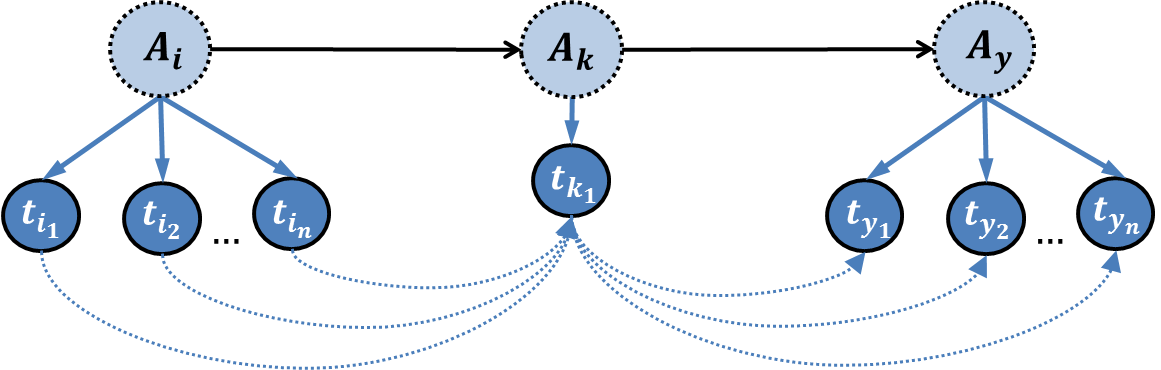
\includegraphics[width=0.8\linewidth]{figure/wf_exec.png}
\caption{Representação das tarefas de um \textit{Workflow} Científico.}
\label{fig:wfexec}
\end{figure}

% FALAR DO Sistema de Gerenciamento de Workflows Científicos.




\section{Nuvens Computacionais}\label{sec2:cc}
Ao longo dos últimos anos várias definições para nuvens computacionais foram apresentadas \cite{Dikaiakos09, Armbrust10, Vaquero08}. Essas definições variam entre o ponto de vista técnico, que aborda os conceitos relacionados a arquitetura e a implementação do ambiente físico e virtual, e o ponto de vista de usabilidade, focado essencialmente nos serviços prestados e nos modelos de cobrança \cite{juve09}. Segundo a ótica de serviço, as nuvens computacionais são um conjunto de servidores virtuais que trabalham interligados através da Internet, e podem ser dinamicamente gerenciados e monitorados \cite{hoffa08}. Esses ambientes se assemelham aos \textit{clusters} nos aspectos técnicos, porém, diferente destes, os recursos computacionais são oferecidos através de virtualização e seguem o modelo de pagamento pague-pelo-uso (do inglês, \textit{pay-per-use}), no qual os usuários são cobrados pelo tempo de uso dos recursos contratados \cite{juve09}.  
 
As nuvens computacionais oferecem várias vantagens técnicas e econômicas em relação as outras plataformas (como \textit{grids} e \textit{clusters}), pois combinam virtualização e escalabilidade em modelos de serviços economicamente viáveis \cite{juve09}. Entre as principais vantagens do uso desse ambiente estão \cite{Hashem15}: processamento paralelo sob demanda; ilusão de recursos infinitos;  e serviços integrados de processamento de dados e armazenamento escalável. Segundo Hashem \textit{et al.} \cite{Hashem15}, além do potencial em diminuir os custos ligados a automação e processamento de dados para indivíduos e empresas, as nuvens computacionais podem reduzir significantemente os custos de aquisição, manutenção, gerenciamento e acesso a infraestruturas computacionais. 

Os serviços prestados pelas nuvens são divididos em três categorias \cite{Hashem15}:

\begin{itemize}
    \item Plataforma como serviço (PaaS, do inglês \textit{Platform as a Service}), que consiste em diferentes recursos (sistemas operacionais, bibliotecas, compiladores, etc.) operando em conjunto para fornecer uma plataforma ao usuário final. Google Apps Engine \cite{gappEngine} e Microsoft Azure \cite{msazure}, são exemplos deste serviço.
    \item \textit{Software} como serviço (SaaS, do inglês \textit{Software as a Service}), consiste em aplicações operadas remotamente em uma infraestrutura de nuvem e oferecidas como um serviço. Exemplos deste modelo são Google Docs \cite{docs}, Gmail \cite{gmail}, Sharelatex \cite{sharelatex}, etc.
    \item Infraestrutura como serviço (IaaS, do inglês \textit{Infrastructure as a Service}, refere-se a equipamentos de \textit{hardware} virtualizados que são fornecidos sob demanda por um provedor de nuvem. Neste modelo, o cliente tem controle total de configuração e instalação de \textit{softwares} no \textit{hardware} adquirido. Amazon EC2 \cite{AmazonEC2}, Google Cloud Platform \cite{gcloud}  e Microsoft Azure \cite{msazure} são exemplos de IaaS.
\end{itemize}


A virtualização é umas das principais tecnologias por trás do sucesso das nuvens computacionais, e pode ser definida como um processo de compartilhamento de recursos computacionais (como CPU, espaço de armazenamento e rede) que isola o \textit{hardware} físico, diminuindo a ineficiência na alocação e distribuição de seus recursos \cite{Hashem15}. O uso mais comum de virtualização é através das máquinas virtuais (MVs), que criam ambientes de \textit{hardware} e \textit{software} configurados de forma totalmente independente do recurso físico, o que permite que várias MVs independentes sejam executadas ao mesmo tempo sob um mesmo \textit{hardware} \cite{hoffa08}. A Amazon EC2, por exemplo, utiliza MVs para oferecer \textit{hardware} virtualizado com diferentes capacidades de memória, largura de banda e poder de processamento. As MVs são classificadas conforme o propósito de uso e capacidade de recursos, e apresentam custo monetário variável. Atualmente, A MV mais barata oferecida pela Amazon EC2 é chamada de t2.nano, e custa $\$0.0059$ hora. A máquina contém um processador virtual (vCPU) baseado no Intel Xeon e 500MB de memória RAM. Já a máquina mais cara, chamada de d2.8xlarge, tem custo de $\$5.52$ hora, 36 vCPUs (também baseadas  no Intel Xeon) e 244 GB de memória RAM \cite{AmazonEC2}.

O uso dos serviços de nuvem para o processamento de aplicações distribuídas se baseia no modelo e IaaS e é feito através da alocação de um \textit{cluster} virtual, que pode ser composto por máquinas de um mesmo tipo (ambiente homogêneo) ou por máquinas com diferentes configurações (ambiente heterogêneo). Especificamente no caso dos WfCs, o SGWfC é responsável pela alocação das MVs necessárias e pelo planejamento de execução das tarefas do \textit{workflow}, feito pelos algoritmos de escalonamento.

                                                                          
\section{O Problema de Escalonamento de WfCs}\label{sec2:sp}

Segundo Yu \textit{et al.} \cite{Yu2008}, escalonamento é o processo de mapear e gerenciar a execução de tarefas em um ambiente computacional. Portanto, é papel do escalonador definir onde e quando  uma tarefa deverá ser executada, sendo que essa decisão está sujeita às restrições impostas às aplicações e ao ambiente. Segundo Topcuoglu \textit{et al.} \cite{HEFT}, em sistemas distribuídos, o escalonamento eficiente das tarefas é um fator chave para atingir um alto desempenho computacional.

Formalmente, o objetivo do escalonador é alocar um conjunto de tarefas $N = \{tf_1,\allowbreak tf_2,\allowbreak\dots,tf_n\}$ em um conjunto de máquinas $M = \{mv_1, mv_2, \dots, mv_n\}$. O escalonador deve otimizar uma função objetivo $f$, que qualifica a solução encontrada e está sujeito a restrições que, caso não sejam satisfeitas, inviabilizam a solução de escalonamento \cite{tsai14}. Os objetivos mais comuns no escalonamento de WfCs são: minimizar o tempo de execução (\textit{makespan}); minimizar o custo monetário; maximizar o uso dos recursos (balanceamento de carga); e minimizar a ocorrência de falhas. No caso das restrições, limitar o orçamento e definir um prazo de execução, são comumente empregadas \cite{Masdari16}. 

O escalonamento de tarefas em sistemas distribuídos faz parte dos chamados problemas NP-Difícil \cite{Ullman1973}. Isso significa que não há algoritmo conhecido capaz de produzir soluções ótimas em tempo polinomial (a menos que $P=NP$). Por conta disso, as abordagens de escalonamento utilizam geralmente algoritmos de resultado aproximados, chamados de  heurísticas de escalonamento \cite{HEFT, Masdari16, Yu2008}. Essas abordagens não garantem que a solução encontrada seja ótima, isto é, a melhor solução possível para o problema. No entanto, são capazes de encontrar soluções com qualidade aceitável, em tempo viável de execução \cite{Kalra15}. As heurísticas são classificadas em diferentes categorias, conforme o critério utilizado na manipulação das tarefas. Uma dessas categorias são os métodos randômicos de busca guiados, chamados também de metaheurísticas \cite{Kalra15, Bossaid13, tsai14}. Segundo Boussaïd \textit{et al.} \cite{Bossaid13}, metaheurísticas são algoritmos elaborados para resolver, de forma aproximada, um grande número de problemas difíceis de otimização sem que seja necessário realizar adaptações profundas no algoritmo para cada um destes problemas. 

Os algoritmos de escalonamento podem ser estáticos ou dinâmicos \cite{Fakhfakh14}. Nos algoritmos estáticos todo o plano de escalonamento é definido antes de qualquer execução. Para isso, os algoritmos consideram as condições iniciais do ambiente (como capacidades de processamento, número de máquinas e taxas de transferência) e não preveem mudanças destas condições ao longo da execução.  Portanto, todas as informações relacionadas ao \textit{workflow} e ao ambiente, como tempo de execução das tarefas, tamanho dos dados e relações de dependências, devem ser conhecidas \textit{a priori} e fazem parte da entrada do problema. A acurácia dessas informações influencia diretamente no resulto do escalonamento, já que informações discrepantes induzem o escalonador ao erro e resultam em soluções de baixa qualidade. As formas mais comuns de obter essas informações é através de execuções prévias do \textit{workflow}, ou com estimativas por modelos matemáticos e testes de \textit{benchmark}.

Nos algoritmos dinâmicos, o escalonamento  é realizado durante a execução do \textit{workflow}. Nessa abordagem, as tarefas são escalonadas por etapas, conforme a disponibilidade do ambiente e das tarefas. Para isso, o escalonador monitora o status de execução e das máquinas e, caso haja tarefas prontas para serem escalonadas e máquinas ociosas, submete as tarefas para a execução conforme um critério de escalonamento que atenda ao objetivo desejado. Normalmente, essa abordagem é local, isto é, o escalonador utiliza as informações das tarefas prontas e das máquinas livres para determinar a alocação, e não considera todo o \textit{workflow} na decisão \cite{Fakhfakh14, Kalra15}. Diferente do escalonamento estático, as informações utilizadas no escalonamento são atualizadas de tempos em tempos, o que melhora a acurácia delas, já que as ocilações de qualidade do ambiente são facilmente detectadas e o escalonamento pode ser adaptado. Embora o escalonamento dinâmico seja mais flexível e exija menos parâmetros de entrada, seu \textit{overhead} de execução e a complexidade na implementação são maiores quando comparados aos algoritmos de escalonamento estático \cite{Fakhfakh14}.





\chapter{Revisão Bibliográfica}\label{chap3}

Este capítulo apresenta o levantamento bibliográfico efetuado ao longo do trabalho. Os artigos apresentados foram divididos em dois tópicos principais: estratégias de escalonamento de tarefas de \textit{workflows} em 
ambientes distribuídos (Seção \ref{sec3:ws});  e estratégias de escalonamento com alocação de dados (Seção \ref{sec3:tds}).  

\section{Estratégias de Escalonamento de tarefas de \textit{workflows} em Ambientes Distribuídos}\label{sec3:ws}

Os algoritmos de escalonamento podem ser divididos em dois grupos de interesse \cite{Smanchat}: algoritmos direcionados ao usuário e algoritmos direcionados ao provedor. A principal diferença entre esses grupos é em relação aos objetivos do escalonamento, isto é, enquanto os algoritmos do lado provedor concentram-se principalmente nas camadas físicas, como distribuição da carga entre os \textit{data centers} e a minimização dos gastos energéticos, os orientados aos usuários concentram-se nos atributos relacionados a contratação dos serviços, como o tempo de execução das aplicações e os custos monetários associados ao uso dos recursos. Como a proposta deste trabalho é voltada aos interesses dos cientistas, este levantamento bibliográfico aborda apenas as soluções de escalonamento voltadas aos usuários. Para auxiliar na leitura, um resumo dos trabalhos discutidos é apresentado na Tabela \ref{tab:trabalhos1}.


\subsection{Heurísticas}

Segundo o levantamento feito em \cite{Masdari16}, a maioria das propostas de escalonamento de \textit{workflows} são baseadas em heurísticas. Neste contexto, uma das heurísticas mais utilizadas é o \textit{Heterogeneous Earliest-Finish-Time} (HEFT) \cite{HEFT}. O HEFT é uma extensão   para ambientes heterogêneos dos algoritmos clássicos de \textit{list scheduling} \cite{SCHUTTEN96}. O algoritmo executa o escalonamento em duas fases: \textit{fase de ranqueamento}, que calcula a prioridade de cada tarefa; e \textit{fase de seleção de máquina}, que escolhe uma tarefa de acordo com o valor de prioridade, e a atribui para a máquina na qual seu tempo de execução será o menor. Inúmeras variações do HEFT foram propostas para o escalonamento de WfCs \cite{Yu07,chopra13, durillo12, Durillo14}. Em \cite{Yu07} um algoritmo de escalonamento adaptativo para ambientes de \textit{grids} é apresentado. O algoritmo, chamado de AHEFT, utiliza o escalonamento definido pelo HEFT e executa reescalonamentos caso sejam detectadas mudanças no ambiente, como a adição ou remoção de máquinas. O objetivo do AHEFT é minimizar o \textit{makespan}. Em Chopra e Singh \cite{chopra13}, o escalonamento dado pelo HEFT é também combinado a técnicas de reescalonamento. Porém, diferente de \cite{Yu07}, os autores executam o escalonamento de \textit{workflows} em ambientes híbridos, que combinam nuvens públicas e privadas. O HEFT é utilizado na execução inicial (realizada na nuvem privada), e caso o \textit{makespan} resultante seja maior que o tempo máximo de execução definido pelo usuário, a heurística seleciona um conjunto de tarefas para serem processadas na nuvem pública. 

Em Durillo, Fard e Prodan \cite{durillo12} o \textit{Multi-Objective} HEFT (MOHEFT) é proposto. O MOHEFT computa um conjunto de soluções, chamadas de Fronteira de Pareto. Essas soluções apresentam uma condição de balanceamento, na qual a melhora de um dos objetivos implica na piora de outra. Em \cite{durillo12}, o MOHEFT foi aplicado a ambientes de nuvens públicas, mais especificamente nos serviços da Amazon EC2. O objetivo era minimizar o \textit{makespan} e diminuir os custos financeiros. Em outro trabalho \cite{Durillo14}, o MOHEFT foi avaliado em \textit{clusters} heterogêneos compostos por 100 nós, o objetivo do trabalho foi minimizar o gasto energético e o \textit{makespan}. Em ambas as avaliações o MOHEFT apresentou soluções viáveis e resultados melhores que heurísticas mais simples, como o próprio HEFT por exemplo. Embora os algoritmos baseadas no HEFT considerem aspectos relacionados ao ambiente, como a capacidade de processamento das máquinas e as taxas de transferências, as restrições de armazenamento não são consideradas. Além disso, os algoritmos também não levam em conta a localização dos dados para decidir o escalonamento das tarefas.

O algoritmo guloso MinMin \cite{minmin} também foi utilizado no escalonamento de \textit{workflows}. O algoritmo escalona as tarefas prontas para serem executadas com base nas informações locais, como tempo de execução das tarefas e a capacidade de processamento das máquinas. A cada iteração, o tempo de término de cada tarefa em relação as máquinas disponíveis é estimado, e a tarefa que apresentar o menor tempo é escalonada primeiro. Essas etapas são repetidas até que não haja mais tarefas para serem escalonadas. Segundo Blythe \textit{et al.} \cite{minmin} a ideia por trás da heurística é  garantir que o tempo total de execução seja incrementado aos poucos, de modo que o \textit{makespan} resultante seja minimizado. Porém, como a heurística não considera o grafo na decisão de escalonamento e o modelo de ambiente considera apenas o poder de processamento das máquinas e as taxas de transferências, a solução resultante pode ser de baixa qualidade e até mesmo inviável, caso haja restrições de armazenamento.

Heurísticas baseadas em particionamento de grafo também foram propostas para este problema \cite{Byun2011, Abrishami}. A ideia geral dos algoritmos de particionamento é definir e alocar subgrafos, de modo que restrições e objetivos sejam satisfeitos. Byun \textit{et al.} \cite{Byun2011} apresentou a heurística PBTS (\textit{Partitioned Balanced Time Scheduling}), cujo objetivo é minimizar o  tempo de execução, respeitando um tempo limite definido pelo usuário. O algoritmo constrói o escalonamento iterativamente, com base no período mínimo de contratação das MVs, que é definido pelo provedor da nuvem. No Amazon EC2, por exemplo, esse período é de 60 minutos, ou seja, se a aplicação for executada por 61 minutos, o usuário é cobrado por 2 períodos (120 minutos). O PBTS define, para cada período, o número mínimo de MVs suficiente para executar as tarefas de uma partição. Nessa abordagem, o usuário define um tempo limite de execução para todo o \textit{workflow}, que é então dividido em sub-limites e atribuído para cada partição (subgrafos do \textit{workflow}). O algoritmo considera os tempos de execução das tarefas e de transferência dos dados, e assume que a comunicação entre tarefas é feita exclusivamente via o Amazon S3 (\url{https://aws.amazon.com/pt/s3/}), que é um serviço de armazenamento compartilhado oferecido pela Amazon \cite{AmazonEC2}. Embora o uso do Amazon S3 facilite as trocas de dados entre as tarefas do \textit{workflow}, as alocações individuais dos arquivos entre as máquinas não podem ser exploradas. Além disso, conforme demonstrado por Juve \textit{et al.} \cite{juve2010}, o Amazon S3 apresenta uma baixa performance para \textit{workflows} compostos por pequenos arquivos, o que é comum em WfCs.

A heurística IC-PCP (\textit{IaaS Cloud Partial Critical Paths}) \cite{Abrishami} constrói subconjuntos de tarefas com base nos caminhos críticos do \textit{workflow}. Cada um desses subconjuntos é escalonado para uma MV, escolhida conforme seu valor financeiro e sua capacidade de processamento. Durante a escolha das máquinas virtuais, o algoritmo dá preferencia às máquinas que já estão em uso. Caso seja necessário alocar novas máquinas, a MV mais barata com capacidade de processamento suficiente para executar o subgrupo de tarefas dentro do tempo limite de execução é escolhida. A busca por caminhos críticos e todo o processo de escalonamento é repetido até que não haja tarefas para serem escalonadas. Embora o agrupamento de tarefas seja capaz de reduzir os custos de transferências, a localização dos dados não é implicitamente explorado por essa abordagem.


\subsection{Metaheurísticas}

As metaheurísticas foram largamente empregadas no escalonamento de WfCs em diferentes ambientes distribuídos. Entre as principais metaheurísticas adotadas destacam-se as baseadas em população, tais como, \textit{Particle Swarm Optimization} (PSO) \cite{kennedy95}, \textit{Ant Colony Optinization} (ACO) \cite{dorigo99} e Algoritmos Genéticos (AG) \cite{goldberg1989}.

O PSO é uma metaheurística baseada no comportamento social de animais, como por exemplo um bando de pássaros buscando comida ou um cardume protegendo-se de predadores. No PSO, o movimento das chamadas partículas é análogo ao "caminhar" de um indivíduo sobre o espaço de busca e sua posição, em um dado intervalo de tempo, é baseada na melhor posição conhecida e na posição da melhor partícula do grupo \cite{pandey2010}. Pandey \textit{et al.} \cite{pandey2010} utilizam o PSO como parte de uma heurística dinâmica de escalonamento, cujo objetivo é minimizar o custo financeiro de \textit{workflows} executados em ambientes de nuvens públicas. A abordagem proposta foi capaz de balancear dinamicamente a carga de tarefas entre os recursos disponíveis e apresentou resultados três vezes melhor em relação a heurística avaliada. Em Rodriguez e Buyya \cite{Rodriguez2014} é apresentado um PSO para o escalonamento estático de WfCs em ambientes de nuvem, cujo objetivo é minimizar o custo financeiro atendendo à restrição de tempo de execução imposta pelo usuário. Diferente de \cite{pandey2010}, que considera recursos homogêneos, a solução de \cite{Rodriguez2014} define as MVs que serão contratadas, o período de contratação e o plano de escalonamento. Embora ambos considerem os tempos de transferências dos arquivos na decisão de escalonamento, a distribuição dos dados no ambiente não é levada em consideração pelos escalonadores.


O ACO é uma metaheurística inspirada no comportamento cooperativo desempenhado pelas formigas durante a busca de alimentos \cite{dorigo99}. Essa metaheurística tem sido aplicada com sucesso em vários problemas reais, inclusive em problemas de otimização combinatória. Chen e  Zhang \cite{Chen2009} apresentam uma solução de escalonamento multi-objetivo para \textit{workflows} executados em \textit{grids}. Os autores propõem uma metaheurística baseada no ACO para atender a três dos principais parâmetros de QoS: confiabilidade dos serviços; custo financeiro; e
\textit{makespan}. São definidas três classes de otimização: otimização de confiabilidade; otimização de \textit{makespan}; e otimização de custo. Essas classes buscam maximizar (ou minimizar, no caso do \textit{makespan}) uma métrica de QoS específica e atender as restrições impostas pelas demais métricas. Para a atualização do feromônio, os autores propuseram sete diferentes heurísticas que são selecionadas em tempo de execução, conforme um esquema adaptativo de própria autoria. O algoritmo obteve em média valores de custo financeiro entre 20\% e 30\% menores do que as heurísticas avaliadas. Em \cite{Hu2010}  o  algoritmo \textit{knowledge-based ant colony optimization} (KBACO) é apresentada. O KBACO constrói escalonamentos estáticos para \textit{workflows} em \textit{grids} utilizando a metaheurística ACO juntamente com heurísticas que utilizam o aprendizado acumulado a cada etapa da construção para melhorar as decisões de escalonamento. O escalonamento deve garantir que um limite de tempo de execução imposto pelo usuário ao \textit{workflow} seja atendido. Ambas as abordagens não consideram as características da rede (taxa de transferência, por exemplo) na decisão de escalonamento.  

Yu e Buyya \cite{Yu2006} apresentaram um GA para o problema de escalonamento estático de \textit{workflows} para ambientes de nuvem.
Nessa proposta, o usuário pode definir qual restrição (tempo máximo de execução ou custo monetário máximo) a metaheurística deverá atender. A solução é representada por uma codificação bidimensional (máquinas x tarefas), e os métodos \textit{Best-fit} e \textit{Round-Robin} são empregados para gerar a população inicial. As abordagens clássicas de  troca e recombinação em dois pontos são empregadas no operador de mutação e no de \textit{crossover}, respectivamente. 


\section{Estratégias de Escalonamento de Tarefas e Alocação de Dados para WfCs}\label{sec3:tds}

Alguns trabalhos consideraram o impacto causado pelas transferência de dados no tempo de execução dos \textit{workflow}, outros, chamados de \textit{data-aware}, executam o escalonamento dos dados e das tarefas, de forma separada.

Em Szabo \textit{et al.} \cite{Szabo2013}, o impacto das transferências de dados no escalonamento de WfCs é discutido. Os autores argumentam que por conta do aumento no volume de dados transferidos entre as tarefas de um \textit{workflow}, as soluções de escalonamento devem considerar a relação entre dados e tarefas para definir o plano de escalonamento. Os autores apresentaram um algoritmo evolutivo que otimiza o escalonamento de tarefas tendo em vista a diminuição das transferências  entre essas e a minimização do tempo de execução do \textit{workflow}. Nesse trabalho, um modelo de transferência e de armazenamento de dados baseado no Amazon S3 é empregado. Além disso, a distribuição dos dados é definida conforme a  alocação das tarefas, isto é, os arquivos de saída das tarefas são escritos tanto no S3, quanto na máquina associada a tarefa. Como resultado, apenas as tarefas alocadas para essa mesma máquina tiram vantagem da alocação dos arquivos, sendo que as outras tarefas devem fazer o \textit{download} diretamente do S3. 

% In  Szabo \textit{et al.} \cite{Szabo2013}, the impact of data transfer in the scheduling of data-intensive scientific workflows is discussed. The authors argue that since the volume of data transferred between tasks of workflows have increased a lot,  the  data  and  task assignment problems  can not be treated independently. The authors propose an evolutionary algorithm that optimizes the task scheduling aiming at minimizing the data transfer among tasks and  the total execution time of the workflow. 

% The metaheuristic proposed by Szabo \textit{et al.} uses a storage and data transfer model based on Amazon S3. Moreover, the file  allocation is driven only by the task assignment, i.e.,  the  output file is  written both in the S3 and in the machine  where the task that generated it is assigned. As a result, only tasks that were allocated to the same machine can take advantage of that file allocation.   Others tasks have to download the file  from the shared storage S3. In our work the allocation of tasks and files considers, among other things, the distribution of all tasks and files in the virtual environment.
% %
% Although it was our intention to compare the results of Szabo \textit{et al.} with ours, the description of the approach given in Szabo's paper did not allow us 
% %to replicate their experiments
% to reproduce the presented results in terms of quality of solutions (the source code was not available either). 
% Thus, in order to present a fair comparison in our paper, we have opted to drop the comparison with Szabo's work and  compare with traditional scheduling approaches such as HEFT \cite{HEFT} and Min-Min \cite{MINMIN}.


Yuan \textit{et al.} \cite{Yuan2010} utiliza uma técnica de clusterização \cite{Broder} baseada em uma matriz de dependência para identificar os arquivos que serão consumidos (isto é, compartilhados) pelas mesmas tarefas do \textit{workflow}. A ideia é armazenar cada arquivo ao \textit{data-center} que contenha o maior número de tarefas que depende deles e, dessa forma, reduzir as transferências entre \textit{data-centers}. O problema de alocação de tarefas e a distribuição dos arquivos não é profundamente explorado pela pelo algoritmo de Yuan \textit{et al.}, pois os escalonamentos de tarefas e arquivos para as MVs dentro de um mesmo \textit{data-center} não são realizados.

% Yuan \textit{et al.} \cite{Yuan2010} use a clustering technique \cite{Broder} based on a dependency matrix to identify  data files which will be consumed (\textit{i.e.} shared) by the same tasks in the workflow. The main idea is to store these data files in the same data center to reduce data transfer between different data centers. It is worth noticing that such approach assigns a task to the data center in which most of the input data is stored. The scheduling task problem and data assignment are not deeply treated in this approach, that ignores the scheduling and data assignment in VMs within the same data center. 

Wang \textit{et al.} \cite{Wang2014} apresenta uma solução cujo objetivo é minimizar as transferência de dados em \textit{workflows} alocados a multiplos \textit{data-centers}. O trabalho define uma localização inicial para os dados estáticos utilizando o algoritmo de clusterização k-means \cite{Broder}. Em seguida, uma técnica de replicação de tarefas é utilizada para reduzir as transferências entre diferentes \textit{data-centers} dos dados produzidos durante a execução do \textit{workflow} (dados dinâmicos). Além da complexidade inerente às técnicas de replicação, como garantir a consistência dos dados, a abordagem proposta por Wang \textit{et al.} não trata dos problemas de transferências dentro de um mesmo \textit{data-center}.

%  Wang \textit{et al.} \cite{Wang2014} present a solution whose objective is to minimize the data transfer of workflows allocated in multiple data centers. This work defines the initial data locality  (\textit{i.e.} static data) by using the k-means clustering algorithm \cite{Broder}. Task replication techniques are used to reduce data transfer, which are generated during  the workflow execution (dynamic data), between different data centers. Besides the intrinsic complexity of replication techniques, such as maintenance of data consistency,  the approach proposed by Wang \textit{et al.} does no tackle the data transfer problem within data centers.

Bryk \textit{et al.} \cite{Bryk} propôs um modelo para execução de múltiplos \textit{workflows} em ambientes de nuvem. O algoritmo \textit{File Locality-Aware scheduling} (FLA-S), que se beneficia da localização dos dados para aumentar a performance de execução dos \textit{workflows} é apresentado. O algoritmo executa uma alocação dinâmica de tarefas, na qual, a cada etapa, as tarefas prontas para a execução são escalonadas para as MVs disponíveis. O escalonador prioriza algumas tarefas, considerando a localização dos dados, com o objetivo de minimizar as transferências. O modelo considera que os dados sejam armazenados em um sistema de arquivos centralizado e compartilhado. Porém, cada MV mantém localmente uma cópia dos arquivos que foram gerados nela, isto é, pelas tarefas alocadas à ela. Portanto, embora a alocação dos arquivos não seja definida pelo algoritmo, as tarefas que consomem os mesmo arquivos, ou que apresentam relação de dependência, são preferencialmente alocadas à mesma MV, evitando assim transferências entre as máquinas e o sistema centralizado de arquivos.

% Bryk \textit{et al.} \cite{Bryk} propose a model to execute workflow ensembles in clouds. They present
% the File Locality-Aware Scheduling Algorithm, which benefits of data locality to increase the performance of workflow executions. The algorithm executes a dynamic task scheduling, in which, at each step, the tasks that are ready to be executed are scheduled to available VMs. The scheduler prioritizes some tasks, considering the data locality, aiming at minimizing data transfer (\textit{i.e.} it tries to choose a VM "near" to data). The execution model considers that both storing and data transfer use a global storage and each VM keeps only data files generated in it during the workflow execution. Thus, although the file locality is not defined by the scheduling algorithm, tasks that consume the same file are preferably allocated in the same VM that contains such file, avoiding in these cases data transfer between machines.

Çatalyürek {\it et al.} \cite{Catal2011} apresentam um algoritmo para a alocação de dados e tarefas de \textit{workflow} executados na nuvem. O \textit{workflow} é modelado como um hiper-grafo. Um algoritmo de particionamento é proposto, cujo objetivo é dividir o \textit{workflow} em $k$ partes (onde $k$ é o número de máquinas virtuais do ambiente), e associa cada uma delas a uma MV diferente, e minimiza o número de transferências de dados. Além disso, o particionamento deve atingir um balanceamento previamente definido pelo usuário. Os autores não consideram característica do ambiente, tal como capacidade de processamento e de armazenamento e taxas de transferências. Apenas o tamanho total dos arquivos transferidos é utilizado para avaliar a qualidade da solução.

% Çatalyürek {\it et al.} \cite{Catal2011} presented an algorithm that treats data file  and task allocation of   workflows executed in clouds. The workflow is  modeled as a hypergraph. They propose a  partitioning  algorithm whose objective is dividing    the workflow in k parts (where k is the number of virtual machines), each one to be associated to a different virtual machine, and minimizing the number of file transfers. Besides that, the  partition must meet  the balancing previously defined by the user. Their work does not consider environment characteristics such as processing and storage capacity and transfer rates. Only the total size of all transferred files are used  to evaluate the solution quality.


% To the best of author's knowledge, the approach proposed in this article is the first one that considers both task and data as vertices in the workflow graph. This way, we can consider both problems together by proposing a model and an  algorithm to minimize the makespan of workflows in cloud environments. Our approach considers different storage capacity of machines, different tasks execution times and data transfer times in these heterogeneous systems. The following section formalizes the problem considered in this article.



\begin{table}[!ht]
        \caption{Resumo dos trabalhos relacionados.}
         \label{tab:trabalhos1}
         \resizebox{\textwidth}{!}{\begin{tabular}{|l |c |c |c |c |}
            \hline
            \textbf{Ref.} & \textbf{Algoritmo} & \textbf{Objetivos}             & \textbf{Restrições} & \textbf{Ambiente}\\
            \hline\hline
            Yu e Shi \cite{Yu07}           &  AHEFT             &  \textit{Makespan} &    -         & \textit{Grids}\\ 
            Chopra e Singh \cite{chopra13} &  HEFT-Based        &  Custo financeiro  &  Tempo de execução  & Híbrido\\
            Durillo, Fard e Prodan \cite{durillo12} & MOHEFT    & \textit{Makespan} e  custo financeiro &  -      & Nuvem\\
            Durillo, Nae e Prodan \cite{Durillo14} & MOHEFT     & \textit{Makespan} e  consumo de energia&  -     & \textit{Cluster}\\
            Blythe \textit{et al.} \cite{minmin}   & MinMin     & \textit{Makespan}  &     -       &    \textit{Grids}\\  
            Byun  \textit{et al.} \cite{Byun2011}  & PBTS       & \textit{Makespan}  &    Tempo de execução &  Nuvem\\
            Abrishami \textit{at al.} \cite{Abrishami} & IC-PCP &  Custo financeiro & Tempo de execução     &  Nuvem\\
            Pandey \textit{et al.} \cite{pandey2010}        & PSO &     Custo financeiro &  -               &  Nuvem\\
            Rodriguez e Buyya \cite{Rodriguez2014}          & PSO &     Custo financeiro &  Tempo de execução &  Nuvem\\
            Chen e Zhang \cite{Chen2009}                    & ACO & Vários objetivos             &  Várias restrições &  \textit{Grids}\\
            Hu \textit{et al.} \cite{Hu2010}                & KACO&  -                  & Tempo de execução          & \textit{Grids} \\
            Yu e Buyya \cite{Yu2006}                        & GA  &  -                           & Tempo de execução e custo & Nuvem\\
            Szabo \textit{et al.} \cite{Szabo2013}          & GA  &  \textit{Makespan} e tempo de transferência & - & Nuvem\\
            Yuan \textit{et al.} \cite{Yuan2010}            & \textit{Clustering} & Número de transferências    & - &  Nuvem\\
            Wang \textit{et al.} \cite{Wang2014}           & k-means & Número de transferências &   -    &   Nuvem\\
            Bryk \textit{et al.} \cite{Bryk}               & FLA-S   & Número de transferências &   -    &   Nuvem\\
            Çatalyürek  \textit{et al.} \cite{Catal2011}   & Partition & Número de transferências & -    &   Nuvem\\ 
             \hline 
         \end{tabular}}
\end{table}




\chapter{Definição do Problema de Escalonamento de Tarefas e Alocação de Dados de WfCs em Nuvem}\label{chap4}


Neste capítulo, o modelo matemático para o problema de escalonamento de tarefas e alocação de arquivos é apresentado. Primeiramente serão discutidos os modelos relacionados à aplicação e ao ambiente de execução. Em seguida, a formulação matemática proposta é apresentada.


\section{Descrição do Modelo Matemático}

Como apresentado no Capítulo \ref{chap2} (Subseção \ref{sec2:wf}), um WfC é comumente definido como um DAG, no qual as tarefas são representadas como vértices e as dependências entre elas são definidas pelos arcos. Nesse contexto, um algoritmo de escalonamento mapeia a execução de tarefas interdependentes para recursos compartilhados (por exemplo, MVs) \cite{workflow-based-sch}. Geralmente, os métodos de escalonamento encontrados na literatura relacionada consideram que todos os arquivos estarão disponíveis em uma máquina, ou sincronizados entre todas. Diferente dessas abordagens, neste trabalho é proposto um novo modelo para o \textit{workflow} e, baseado neste, o problema de Escalonamento de Tarefas e Alocação de Arquivos de Dados (ETAA) é apresentado. 

O ETAA considera que determinar a máquina na qual os dados gerados serão alocados durante a execução do \textit{workflow} é uma etapa crucial para o problema de escalonamento, pois permite diminuir não só o tempo de execução das tarefas, mas também os tempos de transferências. Além disso, essa abordagem também possibilita que o espaço de armazenamento seja levado em consideração, permitindo assim que cenários mais realísticos (isto é, com espaço de armazenamento finito) sejam considerados. Além disso, motivado pela crescente migração de experimentos científicos para ambientes de nuvens computacionais, o ETAA foi formulado considerando as características desses ambientes.  

    
    % Commonly, a workflow is defined by a Directed Acyclic Graph (DAG) in which each task is represented by a vertex, and each data file or dependency between tasks is represented by an arc between the vertices. In this context, workflow-based scheduling aims at mapping the execution of tasks with dependency constraints on shared resources (\textit{e.g.}, VMs) \cite{workflow-based-sch}.
    % %
    % Usually, the scheduling methods, proposed in related work, consider that all data files are already placed in some machines or are synchronized among all machines. Differently from these approaches, this work proposes a new workflow model and, based on it,  The Task Scheduling and Data Assignment Problem (TaSDAP) is presented.  TaSDAP considers that determining the machine where the data file generated during the workflow execution is  assigned, is  also a crucial step in the workflow scheduling problem.
    % %respecting the storage capacity available in these machines, 
    

    % In the last decade, scientists start migrating their scientific experiments to clouds, where computing resources (infrastructure, platform, and software) are provided to users on demand via Internet \cite{cloud-mot}. 
    % %
    % Motivated by this scenario, we choose to tackle the TaSDAP considering the strength and the potential of cloud environments.
    % %
    % The following Subsections \ref{sec:problemDef} and \ref{math_form} present the application and architecture models for the TaSDAP and the proposed mathematical formulation, respectively.

\subsection{Modelo da Aplicação e do Ambiente} \label{sec:problemDef}

O Problema de Escalonamento de Tarefas e Alocação de Arquivos de Dados (ETAA) considera uma classe de aplicações paralelas representadas por um DAG, denotado por $G =(V, A, a, \omega)$.  Diferente dos trabalhos atuais, os arquivos de dados não são representados como arcos do grafo e sim como parte do conjunto de vértices, da mesma forma como as tarefas. Sendo assim, $V = N \cup D$  consiste no conjunto de tarefas $i \in N$ e de arquivos $d \in D$. Já o conjunto de arcos, que dá a relação de precedência entre tarefas e arquivos, é representado por $A$. Por fim, $a_i$ é a quantidade de trabalho associada com a tarefa $i \in N$, e $\omega_k$ representa o custo associado ao arco $k \in A$. 

O conjunto de tarefas predecessores imediatas da tarefa $i \in N$ é definido como $pred (i) = \{j \in N  \mid   \exists d \in D, \mbox{ tal que }  (j, d) \in A  \wedge (d, i) \in A\}$. De forma similar, o conjunto de sucessores imediatos é dado por $succ (i) = \{j \in N  \mid  \exists  d \in D, \mbox{ tal que } (i, d) \in A   \wedge  (d, j) \in A\}$. No grafo, as tarefas são sempre precedidas e sucedidas por arquivos, como ilustrado na Figura \ref{app_model}, na qual a tarefa $tf_1$ lê o arquivo $d_1$ e $d_2$ que são necessários para a sua execução e escreve $d_3$,  que é então lido pela tarefa $tf_2$. Por fim, o arquivo $d_4$ é escrito por $tf_2$ 

%     The Task Scheduling and Data Assignment Problem (TaSDAP) considers a class of parallel applications represented by DAGs (Directed Acyclic Graphs), and denoted by $G =(V, A, a, \omega)$. Differently from the current mainstream, data files are no longer represented as arcs. They are now represented as the set of vertices, similarly to the tasks. Thus, $V=N \cup D$ consists of tasks $i \in N$ and data files $d \in D$; $A$ stands for the set of arcs, which gives the precedence relation between tasks and data files, $a_i$ is the amount of work associated with task $i \in N$, and $\omega_k$ represents  the cost associated with arc $k \in A$.
% 	%
%     The set of immediate  predecessor tasks of a  task $i \in N$ is defined as $pred (i) = \{j \in N  \mid   \exists d \in D, \mbox{ such  that}  (j, d) \in A  \wedge (d, i) \in A\}$. Similarly, the set of immediate successors is given by  $succ (i) = \{j \in N  \mid  \exists  d \in D, \mbox{ such  that} (i, d) \in A   \wedge  (d, j) \in A\}$.
% 	%
%     In the graph, a task is always preceded and succeeded by a data file as illustrated in  Figure \ref{app_model}, where $task_1$ reads data files $data_1$ and $data_2$ as needed for its execution, and writes $data_3$, which will be read later by $task_2$, which also writes the data file $data_4$.
	
    \begin{figure}[H]
    \centering
    \begin{subfigure}{.45\textwidth}
      \centering
    	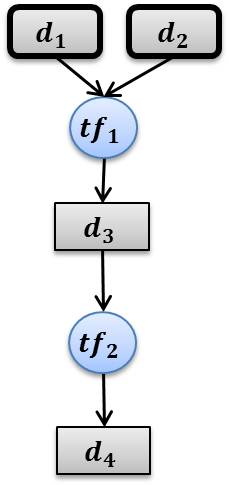
\includegraphics[width=.4\linewidth]{figure/app_model.jpg}
    	\caption{Modelo da aplicação.}
    	\label{app_model}
    \end{subfigure}
    \begin{subfigure}{.5\textwidth}
      \centering
    	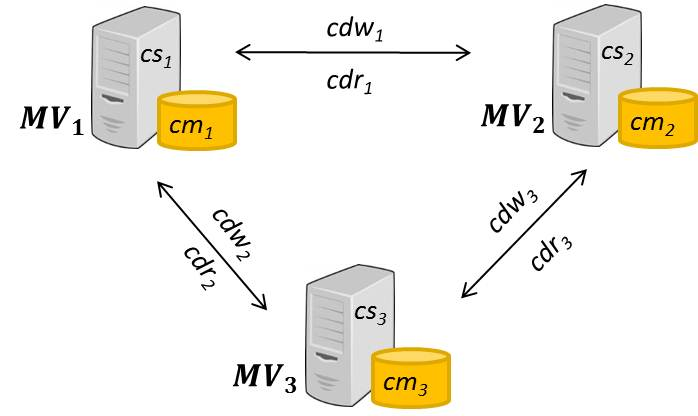
\includegraphics[width=\linewidth]{figure/arch_model1.jpg}
    	\caption{Modelo do Ambiente.}
    	\label{arch_model}
    \end{subfigure}
    \caption{Exemplo dos modelos de ambiente e aplicação.}
    \label{fig:definition}
    \end{figure}

O modelo do ambiente, apresentado na Figura \ref{arch_model}, representa os recursos utilizados durante a execução das aplicações. Nessa representação, o conjunto de todas as MVs disponíveis para execução e armazenamento é dado por $M$. Cada MV $j \in M$ tem capacidade de armazenamento $cm_j$ e um valor computacional de \textit{slowdown} definido como $cs_j$. O \textit{slowdown} representa o grau de diferença da capacidade de processamento das diferentes MVs disponíveis, e é uma alternativa à representação do tempo de execução das tarefas por meio de matrizes \cite{nascimento}. Neste trabalho, o valor de \textit{slowdown} é inversamente proporcional à capacidade de processamento $cp_j$ de uma MV $j$. Porém, nos testes teóricos realizados com \textit{workflows} sintéticos disponíveis na literatura, o valor foi definido em termos dos tempos de execução das tarefas. Essa diferença é explicada no Capítulo \ref{chap6}.



% The architectural model specifies the main features of the target architecture. In order to better reproduce the reality of a large-scale system, let $M$ be the set of all VMs available for execution or storage. Each VM $j \in M$ has a storage capacity $cm_j$ and computational slowdown index $cs_j$, which is inversely proportional to the computational power $cp_j$ of VM $j$, according to Silva \textit{et al.} \cite{nascimento}. 

Seguindo a mesma ideia do \textit{slowdown}, $cd_{l}$  representa o custo de latência associado ao enlace $l$. Dois tipos de retardo de comunicação são propostos: um para a operação de escrita, $cdw_{l}$, e outro para a de leitura, $cdr_{l}$. Por conta disso, duas matrizes de comunicação são construídas, cada uma relacionada a uma das operações de comunicação.  Dessa forma, o tempo de execução da tarefa $i \in N$ na MV $j \in M$ é dado por $t_{ij} = a_i \times cs_j$. Já o tempo de comunicação da tarefa $i \in N$ executando na MV $j \in M$, para escrever e dado $d \in D$ na MV $p \in M$, sendo $j$ e $p$ conectados por um enlace $l$, é dado por $\overleftarrow{t}_{djp} = \omega_{id} \times cdw_{l}$. De modo similar, o tempo de comunicação para leitura é dado por $\overrightarrow{t}_{djp} =  \omega_{di} \times cdr_{l}$. A Figura \ref{arch_model} ilustra um ambiente composto por 3 MVs, contendo as seguintes informações: (i) capacidade de armazenamento $cm$, (ii) valor computacional de \textit{slowdown} $cs$, (iii) o custo de comunicação para operação de escrita ($cdw$) e (iv) o o custo de comunicação para operações de leitura ($cdr$).

A fim de simplificar o modelo, neste trabalho assume-se que um arquivo lido por uma tarefa será mantido na memória principal (volátil). Assim, a operação de leitura não necessita de espaço de armazenamento e não mantém cópia dos dados em diferentes máquinas. 


% 	Moreover, a communication delay index $cd_{l}$ estimates the latency cost associated with each link $l$ of the system. We propose two types of communication delay here. One for the writing cases, $cdw_{l}$, and one for the reading cases, $cdr_{l}$. For supporting our model, two communication delay matrices are built, each one concerning one type of delay. 
%     Therefore, the execution time of a task $i \in N$ on a VM $j \in M$ is given by $t_{ij} = a_i \times cs_j$. 
%     %Let $k \in A$ be an arc connecting task $i \in N$ and data $d \in D$.
%     Furthermore, the communication time for a task $i \in N$ executing on VM $j \in M$, to write data $d \in D$ in VM $p \in M$,  where $j$ and $p$ are connected by link  $l$, is  given by $\overleftarrow{t}_{djp} = \omega_{id} \times cdw_{l}$. Similarly, the communication time for  reading is given by $\overrightarrow{t}_{djp} =  \omega_{di} \times cdr_{l}$. Figure \ref{arch_model} illustrates an example of the architectural model containing three VMs and its characteristics: (i) the storage capacity $cm$, (ii) the computational slowdown index $cs$, (iii) the communication delay index for write operations ($cdw$) and (iv) the communication delay index for read operations ($cdr$).
    
%     Note that when a data is read by some VM, we assume that it is held in main (volatile) memory. Thus, read operations does not require available storage capacity to store data. As future work we intend to tackle the data replication problem in our model. In this way, read operations can take advantage of the nearest replica. 

\subsection{Formulação Matemática}\label{math_form}

O ETAA pode ser formulado como um problema de programação inteira mista, nomeado IP-ETAA, como descrito a seguir. Primeiro, é necessário definir duas classes distintas de arquivos: os arquivos estáticos; e os arquivos dinâmicos. Os arquivos estáticos são aqueles que não são produzidos durante a execução do \textit{workflow} e servem principalmente como entrada para as primeiras tarefas executadas (embora também possam ser utilizados pelas demais tarefas). Um arquivo estático é armazenado antes da execução do \textit{workflow}, em uma das MVs cujo espaço de armazenamento seja suficiente. As alocações desses arquivos não são alteradas em nenhum momento da execução.

Já os arquivos dinâmicos são gerados pelas tarefas como resultado dos processamentos realizados durante a execução do \textit{workflow}. Os arquivos dinâmicos podem ser armazenados em qualquer MV disponível, desde que haja espaço de armazenamento suficiente. A alocação de arquivos, definida como parte do problema deste trabalho, tem a classe de arquivo dinâmicos como foco e, portanto, é papel do escalonador definir a localização desses arquivos.

Sendo assim, $D = D_s \cup D_d$ é definido como sendo o conjunto de todos os arquivos, onde cada arquivo $d \in D$ tem tamanho $W(d)$ e pode ser estático $d \in D_s$ com uma máquina de origem $O(d) \in M$, ou dinâmico $d \in D_d$. Além disso, para cada tarefa $i \in N$ são associados um conjunto de arquivos de entrada $\Delta_{in}(i) \subseteq D$ necessário para sua execução, e um conjunto de arquivos de saída $\Delta_{out}(i) \subseteq D_d$.  Por fim, um tempo $T_M$ é definido como o tempo máximo de execução do \textit{workflow}, sendo $T=\{1 \ldots T_M\}$ o conjunto de intervalos de tempo de uma execução. 

    % The TaSDAP can be formulated as the mixed integer programming problem, named TaSDAP-IP, as described following.
    % Let redefine $D=D_s\cup D_d$ as the set of all data, where each data $d \in D$ has a size $W(d)$ and can be either static ($D_s$), with an origin machine $O(d) \in M$, or dynamic, generated during the workflow execution, ($D_d$). For each $i \in N$,  we consider a set of input data $\Delta_{in}(i) \subseteq D$ needed for it execution and a set of output data 	$\Delta_{out}(i) \subseteq D_d$ generated by it.
    % Moreover, we define $T_M$ as the maximum execution time for the workflow and $T=\{1 ... T_M\}$ as the set of feasible periods.

 
    
    % In this vein, the TaSDAP is defined as the problem of scheduling tasks and assigning data on VMs, respecting the available storage capacity and trying to minimize the makespan. Next, we summarize the data and variables used in the proposed mathematical formulation and present the TaSDAP-IP.
    
    
\begin{table}[h]
\label{tab:desc}\caption{Descrição dos dados e das variáveis utilizadas no modelo matemático.}
\begin{tabularx}{\textwidth}{|l|X|}
\hline
\textbf{Dados}      & \textbf{Descrição}\\
\hline \hline
	$D_s$           &  Conjunto de arquivos estáticos.\\
	$D_d$           &  Conjunto de arquivos dinâmicos.\\
    $D=D_s\cup D_d$ &  Conjunto de arquivos.\\
    $O(d)$          &  Máquina de origem do arquivo estático $d \in D_s$.\\
    $W(d)$          &  Tamanho do arquivo $d \in D$.\\
    $N$             &  Conjunto de tarefas.\\
    $a_i$           &  Quantidade de trabalho da tarefa $i \in N$.\\
    $M$             &  Conjunto de Mvs.\\
    $t_{ij}$        &  Tempo de processamento da tarefa $i \in N$ na Mv $j \in M$. \\
    $\overrightarrow{t}_{djp}$ & Tempo gasto pela Mv $j \in M$ para ler o arquivo $d \in D$ armazenado na Mv $p \in M$\\
    $\overleftarrow{t}_{djp}$  & Tempo gasto pela Mv $j \in M$ para escrever o arquivo $d \in D_d$ na Mv $p \in M$.\\
    $\Delta_{in}(i) \subseteq D$ & Conjunto de arquivos de entrada necessários para a execução da tarefa $i \in N$.\\
    $\Delta_{out}(i) \subseteq D_d$ & Conjnto de arquivos de saída gerados pela tarefa $i \in N$.\\
    $cm_j$          & Capacidade de armazenamento da Mv $j \in M$.\\
    \hline 
    \hline
\textbf{Variáveis}  & \textbf{Descrição}\\
\hline
\hline
    $x_{ijt}$                    & Variável binária que indica se a tarefa $i \in N $ iniciou sua execução na Mv $j \in M$ no período $t \in T$ ou não.\\
    $\overrightarrow{x}_{idjpt}$ & Variável binária que indica se a tarefa $i \in N $ executando na Mv $j \in M$ começou a ler o arquivo  $d \in \Delta_{in}(i)$, que está armazenado na Mv $p \in M$, no período  $t \in T$ ou não.\\
    $\overleftarrow{x}_{djpt}$   & Variável binária que indica se o arquivo $d \in D_d$ começou a ser escrito a partir da Mv $j \in M$ para a Mv $p \in M$ no periodo $t \in T$ ou não.\\
    $y_{djt}$                    & Variável binária que indica se o arquivo $d \in D$ está armazenado na Mv $j \in M$ no período $t \in T$ ou não.\\
    $z_T$                        & Variável contínua que indica o tempo total de execução (\textit{makespan}) do \textit{workflow}.\\
\hline
\end{tabularx}
\end{table}

Como o objetivo do escalonamento é minimizar o tempo total de execução da aplicação, a função objetivo, definida em (\ref{fo}),  minimiza o \textit{makespan} ($z_T$) da aplicação.
% Objetivo
\begin{align}
&\min{z_T} \label{fo}
\end{align}


A restrição (\ref{r1}) garante que cada tarefa seja executada. As restrições (\ref{r2}) e (\ref{r3}) certificam que todas as operações de leitura e escrita sejam realizadas, respectivamente. Já a inequação (\ref{r1}) garante que o dado $d \in \Delta_{out}(i)$ seja escrito apenas se a tarefa $i$ tenha sido executada no tempo correto. Além disso, as restrições definidas em (\ref{r4_1}) asseguram que o dado $d$ não possa ser escrito antes do tempo de processamento da tarefa $i$ (responsável pela sua escrita). Note que ambas as restrições (\ref{r4} e \ref{r4_1}) trabalham em conjunto para garantir um tempo de escrita factível.

% restrições
\begin{align}
&\mathrm{Sujeito\ a\ }  &\nonumber\\
& \sum_{j \in M}\sum_{t \in T} x_{ijt}=1 , & \forall i \in N \label{r1}
\end{align}

\begin{align}
& \sum_{j,p \in M}\sum_{t \in T} \overrightarrow{x}_{idjpt}=1 , & \forall i \in N, \forall d \in \Delta_{in}(i) \label{r2}
\end{align}

\begin{align}
& \sum_{j,p \in M}\sum_{t \in T} \overleftarrow{x}_{djpt}=1 , & \forall d \in D_d \label{r3}
\end{align}

\begin{align}
& \overleftarrow{x}_{djpt} \leq x_{ij(t-t_{ij})} , & \forall d \in D_d, \forall j,p \in M, \nonumber \\ 
&& \forall t = (t_{ij}+1) \cdots T_M  \mbox{ tal que } d \in \Delta_{out}(i)\label{r4}
\end{align}

\begin{align}
& \overleftarrow{x}_{djpt}=0 & \forall d \in D_d, \forall j,p \in M , \nonumber \\ 
&&  1 \leq t \leq t_{ij} \mbox{ tal que } d \in \Delta_{out}(i) \label{r4_1}
\end{align}

A restrição definida em (\ref{r5}) assegura que uma tarefa só possa ser executada quando todas as operações de leitura estiverem concluídas. Além disso, a desigualdade (\ref{r7}) garante que apenas uma ação (execução, leitura ou escrita) possa ser realizada em cada período de tempo em cada MV. Ou seja, a MV não pode executar uma tarefa e escrever, ou ler, um dado ao mesmo tempo.




\begin{align}
& x_{ijt} \leq \sum_{p \in M} \overrightarrow{x}_{idjp(t-\overrightarrow{t}_{djp})} , &\forall i \in N, \forall d \in \Delta_{in}(i), \forall j \in M,\nonumber\\
&& \forall t \in T, \mbox{ tal que }  (t-\overrightarrow{t}_{djp})\geq 1 \label{r5}
\end{align}

\begin{align}
& \sum_{i \in N} \sum_{q=\max{(1,t-t_{ij}+1)}}^t x_{ijq} +  \sum_{d \in D_d} \sum_{p \in M} \sum_{r=\max{(1,t-  \overleftarrow{t}_{djp}+1)}}^t \overleftarrow{x}_{djpr} + &   \nonumber\\
& \sum_{i \in N} \sum_{d \in \Delta_{in}(i)} \sum_{p \in M} \sum_{r=\max{(1,t-  \overrightarrow{t}_{djp}+1)}}^t \overrightarrow{x}_{idjpr} \leq 1 , & \forall j \in M, \forall t \in T  \label{r7}
\end{align}


A restrição (\ref{r8}) estabelece que não há arquivos dinâmicos no tempo inicial. Por outro lado, a restrição (\ref{r9}) garante que todos os arquivos estáticos estejam prontamente armazenados em suas máquinas de origem. Já as restrições (\ref{r10}) e (\ref{r11}) relacionam a variável de armazenamento $y$ com as variáveis de escrita $\overleftarrow{x}$ e de leitura $\overrightarrow{x}$, garantindo um processo viável de escrita e leitura. A restrição (\ref{r11}) garante que os arquivos serão lidos apenas se estes estiverem previamente armazenados em uma MV, e a restrição (\ref{r10}) assegura que um arquivo seja armazenado em MV apenas caso ele tenha sido produzido (escrito).



\begin{align}
& y_{dj1} =0, & \forall d \in D_d, \forall j \in M \label{r8}
\end{align}

\begin{align}
& y_{djt} =1, & \forall d \in D_s \mid j \in O(d), \forall t \in T \label{r9}
\end{align}

\begin{align}
& y_{dp(t+1)} \leq y_{dpt} + \sum_{j \in M} \overleftarrow{x}_{djp(t-\overleftarrow{t}_{djp})} &, \forall d \in D, \forall p \in M, \nonumber\\
&&\forall t \in T, \mbox{ tal que } (t-\overrightarrow{t}_{djp}) \geq 1 \label{r10} 
\end{align}



A capacidade de armazenamento das MVs é estabelecida pela restrição (\ref{r12}). A restrição (\ref{r13}) relaciona a última operação de escrita com o tempo total de execução da aplicação (\textit{makespan}). Note que no modelo da aplicação, uma tarefa sempre escreve ao menos um arquivo. Além disso, a restrição operacional (\ref{r15}) deve ser satisfeita: uma tarefa $i$ pode iniciar um processo de leitura se todos os arquivos $d \in \Delta_{in}(i)$ estiverem disponíveis (isto é, se todos os arquivos $d \in (\Delta_{in}(i) \cap D_d)$ forem escritos). Por fim, as restrições restantes são as de integralidade e de não negativação.



\begin{align}
& \sum_{j \in M} \overrightarrow{x}_{idjpt} \leq y_{dpt} &, \forall i \in N, \forall d \in \Delta_{in}(i), \forall p \in M, \forall t \in T \label{r11}
\end{align}

\begin{align}
& \sum_{d \in D} y_{djt} W(d) \leq cm_j & , \forall j \in M, \forall t \in T \label{r12}
\end{align}

\begin{align}
& \overleftarrow{x}_{djpt}\cdot (t+\overleftarrow{t}_{djp}) \leq z_T & , \forall d \in D_d , \forall j,p \in M, \forall t \in T \label{r13}
\end{align}

\begin{align}
& \overrightarrow{x}_{idjpt} \cdot |\Delta_{in}(i) \cap D_d| \le \sum_{g \in \{\Delta_{in}(i) \cap D_d\}}\sum_{l,o \in M} \sum_{u=1}^{t-\overleftarrow{t}_{glo}}\overleftarrow{x}_{glou} & , \forall i \in N, \forall d \in \Delta_{in}(i), \nonumber \\
&&\forall j,p \in M, \forall t \in T \label{r15}
\end{align}







    % The objective function (\ref{fo}) minimizes the application makespan. 
    % %
    % Constraints (\ref{r1}) guarantee that every task must be executed. Constraints (\ref{r2}) and (\ref{r3}) rule that every read and write operations must be accomplished, respectively. 
    % % %
    % Inequalities (\ref{r4}) guarantee that data $d \in \Delta_{out}(i)$ can only be written, if task $i$ was executed in the correct time. Furthermore, constraints (\ref{r4_1}) rule that data $d$ can not be written before the processing time of the task $i$ (responsible for its writing). Note that both sets of constraints ((\ref{r4}) and (\ref{r4_1})) work together to guarantee a feasibly time for the writing process.
    %
    % Constraints (\ref{r5}) rule that a task can only be executed, if all necessary readings were concluded in a feasible time.
    % %
    % Inequalities (\ref{r7}) guarantee that only one action (execution, reading or writing) can be accomplished at each period of time in each VM (e.g. a VM cannot execute a task and write data at the same time). 
    % %
    % Constraints (\ref{r8}) establish that there are no dynamic data at starting time. On the other hand, constraints (\ref{r9}) guarantee that all static data are already stored on its origin machines. 
    % %
    % % Constraints (\ref{r10}) and (\ref{r11}) link the storage variable $y$ with the write variable $\overleftarrow{x}$ and the read variable $\overrightarrow{x}$, guaranteeing a feasible write and read process, respectively.
    % %
    % In detail, constraint (\ref{r11}) ensures that data will only be read if previously stored in a VM, and constraint (\ref{r10}) ensures that data will only be stored in a VM, if it has been already produced (written). 
    
    % The VMs storage capacity are bounded by constraints (\ref{r12}).
    % %
    % Constraints (\ref{r13}) relate the last write operation with the application execution time (makespan). Note that in our application model a task always creates data.
    % %
    % Moreover, the following operational constraint (\ref{r15}) must be satisfied: a task $i$ can only begin any reading process if all data $d \in \Delta_{in}(i)$ is already available (\textit{i.e.}, if all data $d \in (\Delta_{in}(i) \cap D_d)$ is written).
    % %Constraints (\ref{r14}) make sure that a data replication occurs from a machine that has the content.
    % %
    % Finally, the remaining constraints are the integrality and non-negativity constraints.
%
\chapter{Algoritmo Evolutivo Híbrido Para o Escalonamento de Tarefas e Alocação de Arquivos}\label{chap5}

Este capítulo apresenta o AEH-ETAA, um algoritmo evolutivo híbrido que soluciona o problema de escalonamento de WfCs em ambientes de nuvens computacionais conforme o modelo matemático proposto neste trabalho. O algoritmo é apresentado  em função de seus principais métodos, discutidos em detalhes nas seções que seguem.



\section{AEH-ETAA}

Algoritmos Evolutivos (AE) \cite{Moraglio2012} são métodos de otimização inspirados nos mecanismos de evolução biológica observados na natureza. No AE, cada cromossomo é um indivíduo de uma população e representa uma possível solução para o problema. A busca pela melhor solução é guiada por uma função de \textit{fitness}, que atribui qualidade aos cromossomos. A cada iteração do algoritmo, novos indivíduos são gerados através da operação de \textit{crossover} e a diversidade da população é obtida através da função de mutação. Neste trabalho, um Algoritmo Evolutivo Hibrido (AEH) que combina os operadores do AE,  buscas locais e um método de \textit{path relinking} \cite{Reeves1998} foi desenvolvido. De acordo com Moscato e Cotta \cite{Moscato2010}, diferente do AE tradicional o AEH explora os conhecimentos disponíveis sobre o problema para atingir melhores resultados.

O Algoritmo Evolutivo Híbrido para Escalonamento de Tarefas e Alocação de Arquivos (AEH-ETAA) é uma metaheurística que escalona WfCs em ambientes de nuvens computacionais. Diferente da maioria das abordagens apresentadas na literatura, o AEH-ETAA é responsável por determinar tanto a alocação das tarefas, quando a localização dos arquivos gerados durante a execução do \textit{workflow}. Essa abordagem dá maior flexibilidade para o escalonador, pois permite que o tempo total de execução do \textit{workflow} possa ser minimizado considerando tanto a execução das tarefas, como também os tempos gastos em transferências de arquivos. 

O Algoritmo \ref{algo:HEA} representa o procedimento \textit{Principal} do AEH-ETAA, que é responsável pela chamada dos demais procedimentos. Como pode ser visto, a metaheurística é composta pelas seguintes operações: (i) geração da população inicial (Subseção \ref{sssec:initialPopulation}); (ii) buscas locais (Subseção \ref{ssec:localSearch});  e  (iii) \textit{path relinking} (Subseção \ref{ssec:pr}). Além disso, também é definido o procedimento \textit{GeraPopulação} (apresentado no Algoritmo \ref{algo:doPop}), que é responsável pela criação de novas soluções durante a execução da metaheurística. Esse procedimento é composto pelas operações de \textit{crossover} e mutação (Subseções \ref{ssec:crossover} e \ref{ssec:Mutation}, respectivamente).


 \begin{algorithm}
 \caption{Procedimento Principal}\label{algo:HEA}

\begin{algorithmic}[1]
\Require Informações do \textit{workflow} e do Ambiente.
\Ensure Melhor solução encontrada (\textit{best\_global}).

\State $P \gets  \textit{populaçãoInicial}()$
\State $best\_global \gets encontraBest(P)$ 
\State $ConjElite \gets \emptyset$ 
\State $i \gets 0$ 

\While{$i \leq MAX$}
    \If{$fazBuscasLocais?$}\label{l:checkbl}
        \State $P \gets \textbf{buscasLocais}(P)$ \Comment{ Algoritmos \ref{algo:trocamv}, \ref{algo:trocapos}, \ref{algo:moveelem}.}
    \EndIf
    
    \State $ best\_atual \gets encontraBest(P)$ 
    
    \If{$ fitness(best\_atual) \textbf{ melhor que } fitness(best\_global) $}
    
        \State $best\_global \gets best\_atual$
        
        \If{$ConjElite \neq \emptyset $} \label{l:path1}
            \State $best\_global \gets \textbf{pathRelinking}(best\_global, conjElite)$ \label{l:path2} \Comment{Algoritmo \ref{algo:pr}.}           
        \EndIf
        
            
        \If{$ \forall \textit{solução} \in ConjElite, \textit{distância}(best\_global, \textit{solução}) \geq \alpha $} 
            \State $ConjElite \gets ConjElite \cup best\_global$ 
            \If{$|conjElite| > \beta$} \label{l:remove1}
                \State $\textit{removeCromossomo(ConjElite)}$ \label{l:remove2}
            \EndIf
        \EndIf    
    \EndIf
        
        \State $P \gets \textbf{geraPopulação}(P)$ \Comment{Algoritmo \ref{algo:doPop}}
        \State $i = i + 1$
        
\EndWhile
    
\State \textbf{retorna} $best\_global$

\end{algorithmic}
\end{algorithm}



\begin{algorithm}[H]
\caption{Procedimento  GeraPopulação}\label{algo:doPop}

\begin{algorithmic}[1]
\Require População Anterior (P).
\Ensure Próxima População (P').

    \State $Filhos \gets \emptyset$

    \For{$i \gets 1$ \textbf{a} $NUM\_OFFSPRING$}
         \State $p_1 \gets \textit{torneio(P)}$
         \State $p_2 \gets \textit{torneio(P)}$
         \State $novo \gets \textbf{crossover}(p_1, p_2)$ \Comment{ Algoritmo \ref{algo:crossover}}
         \State $novo' \gets \textit{mutação(novo)}$ \label{l:mut}
         \State $\textit{\textbf{calculafitness}}(novo')$ \Comment{Algoritmo \ref{algo:fitness}}
         \State $Filhos \gets Filhos \cup novo'$         
    \EndFor

    \State $\textit{Soluções} \gets Filhos \cup \textit{P}$  \label{l:selecaoInit}
    \State $P' \gets \textit{selecionaBests(Soluções)}$ \Comment{Componente elitista.} \label{l:elitism}
    
    \While{$|P'| < \textit{POPULAÇÃO\_MAX}$}
        \State $cromossomo \gets \textit{torneio(Soluções)}$
        \State $P' \gets P' \cup cromossomo$
        \State $\textit{Soluções} \gets \textit{Soluções} \setminus cromossomo$ \label{l:selecaoFim}
    \EndWhile 

    \State \textbf{retorna} $P'$

\end{algorithmic}
\end{algorithm}


\subsection{Representação do Cromossomo} \label{sssec:encode}
 
Como apresentado no Capítulo \ref{chap4}, no problema de escalonamento de tarefas e alocação de arquivos de dados (ETAA), uma solução viável deve respeitar as ordens de precedência entre as tarefas, que são definidas através das relações de leitura e escrita presentes no \textit{workflow}. Em outras palavras, uma tarefa $tf_i$ só pode ser executada quando todos os seus arquivos de entrada estiverem disponíveis. Essa situação ocorre em dois cenários: (i) quando todas as tarefas predecessoras de $tf_i$ estiverem finalizadas e, portanto, todos os seus arquivos de saída já estiverem disponíveis; ou (ii) quando $tf_i$ tiver como entrada arquivos estáticos que, conforme a definição do modelo, estão disponíveis durante toda a execução do \textit{workflow}. Por exemplo, na Figura \ref{fig:height}, a tarefa $tf_2$ depende do arquivo gerado por $tf_0$. Sendo assim, $tf_2$ só poderá ser executada após a finalização de $tf_0$.

Neste trabalho, um cromossomo é composto por duas estruturas que representam: (i) a alocação das tarefas e dos dados e (ii) a ordem de execução das tarefas. Essa representação foi inspirada nas ideias apresentados em Szabo \textit{et al.} \cite{Szabo2013}, e permite que os procedimentos de buscas locais e o cálculo do \textit{fitness} sejam facilmente realizados.
Como pode ser visto na Figura \ref{fig:encoding}, a primeira estrutura é um vetor no qual os índices representam tarefas ou arquivos dinâmicos, e cada elemento representa a MV na qual a tarefa, ou o dado, foi alocado. Essa estrutura é chamada de \textit{vetor de alocação}. 


A representação da alocação de dados nesse vetor é uma importante diferença entre este trabalho e a literatura relacionada. É essa a estrutura que permite que a metaheurística proposta trate não apenas do problema da alocação de tarefas, mas também da alocação dos dados.


\begin{figure}[H]
    \centering
    \begin{subfigure}{0.6\textwidth}
    \centering
        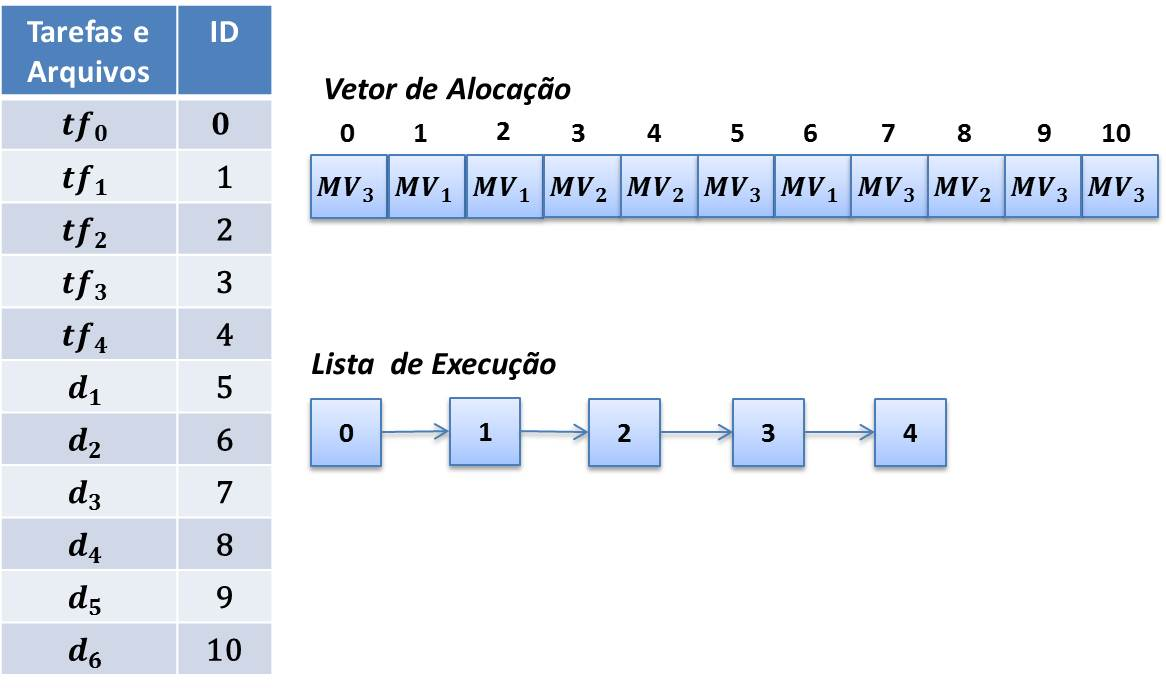
\includegraphics[width=1\linewidth]{figure/representacao.jpg}
        \caption{Estruturas de dados para representação do cromossomo.}
        \label{fig:encoding}
        \vspace{2\baselineskip}
    \end{subfigure}
    \begin{subfigure}{0.6\textwidth}
    \centering
        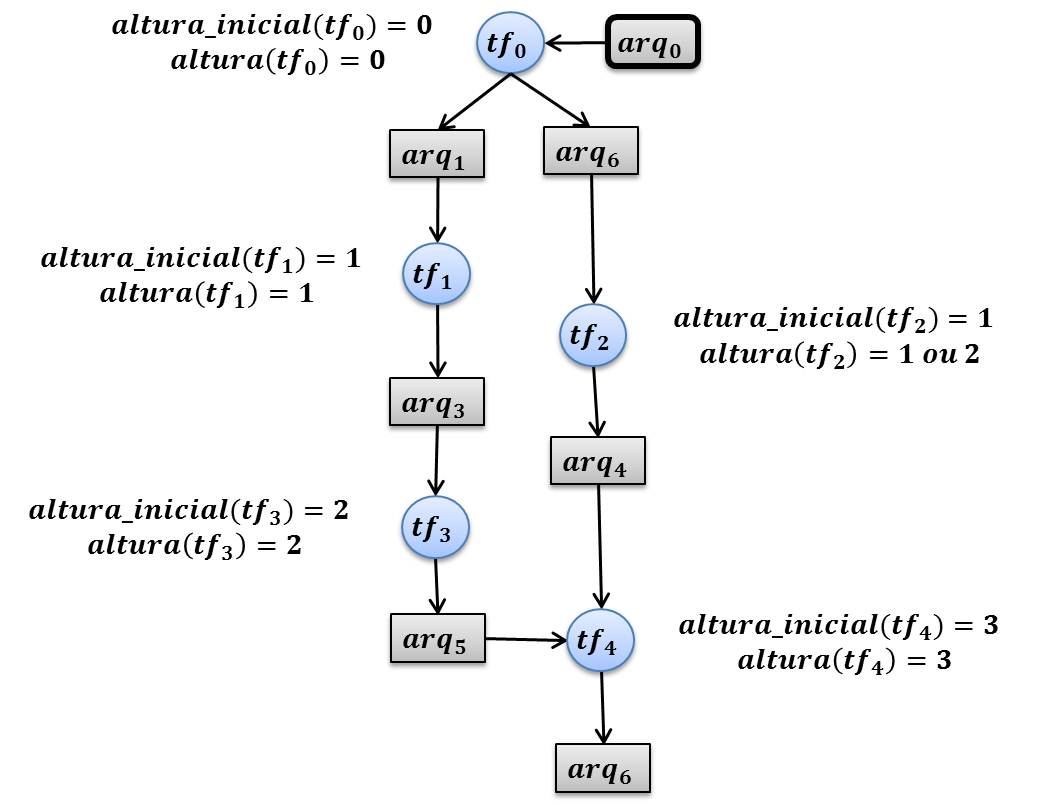
\includegraphics[width=0.9\linewidth]{figure/height.jpg}
        \caption{Cálculo da altura das tarefas.}
        \label{fig:height}
    \end{subfigure}
    \caption{Codificação do cromossomo.}
    \label{fig:representation}
    \end{figure}


A ordem de execução das tarefas é representada por uma lista encadeada chamada de \textit{lista de execução}, presente também  na Figura \ref{fig:encoding}. Para definir a ordem de execução das tarefas, um valor de altura é associado a cada uma delas. Uma tarefa só pode ser executada quando todas as tarefas de altura menores que a dela estiverem finalizadas. Já as tarefas com altura semelhante executam concorrentemente. O valor de altura é dado pelas equações \ref{eq:height}  e \ref{eq:heights}, propostas por Tsujimura e Gen \cite{Tsujimura1997}.

\begin{equation}
\label{eq:height}
\resizebox{0.8\textwidth}{!}
{
\text{$altura\_inicial(tf_i)$} = \begin{cases}
                            0, &\text{se } pred(tf_i) = \emptyset\\
                            1 + \max\limits_{tf_j \in pred(tf_i)}{altura\_inicial(tf_j)}, & \text{caso contrário}
                        \end{cases}
}
\end{equation}


\begin{equation}
\label{eq:heights}
\resizebox{0.8 \textwidth}{!} 
{
 
\text{$altura(tf_i)$}  = \begin{cases}
                altura\_inicial(tf_i),  &\text{se } suc(tf_i) = \emptyset\\
                    rand \in [altura\_inicial(tf_i), \min\limits_{\forall tf_k \in suc(tf_j)}{\{altura(tf_k)\}} - 1], &\text{caso contrário}
                  \end{cases}

}
\end{equation}


A equação \ref{eq:height} atribui para cada tarefa uma altura inicial correspondente ao nível no qual a tarefa aparece no grafo que representa o \textit{workflow}; a altura é zero quando não há predecessor, ou o máximo entre todas alturas iniciais de seus predecessores mais um. Essa equação permite que seja realizada uma ordenação topológica do grafo, já que basta definir grupos de tarefas de mesma altura (ou seja, que estão no mesmo nível) e, com base nos valores atribuídos, ordenar esses grupos de forma crescente. Porém, caso as tarefas sejam ordenadas apenas com base na altura inicial dada pela equação \ref{eq:height}, o paralelismo entre diferentes grupos de tarefas não seria explorado. Por exemplo, na Figura \ref{fig:height}, a tarefa $tf_2$ pode ser executada em paralelo tanto com $tf_1$ quanto com $tf_3$, pois não há relação de dependência entre essas tarefas. No entanto, a ordenação com base na altura inicial sempre atribuirá a altura de valor $1$ para $tf_2$, permitindo apenas o paralelismo entre $tf_2$ e $tf_1$. 

% At first, equation (\ref{eq:height}) assigns to a task an initial height corresponding to the order in which it can be executed; it can be zero when it has no predecessors, or the maximum of the initial heights among all predecessors plus one.

Para permitir que o paralelismo entre as tarefas seja totalmente explorado, um componente randômico é introduzido na equação \ref{eq:heights}. Esse componente permite que a tarefa possa ser executada em qualquer ordem entre a altura previamente calculada (altura inicial) e o valor mínimo da altura inicial de seus sucessores menos um. Seguindo o exemplo anterior, com o cálculo da Equação \ref{eq:heights} a tarefa $tf_2$  pode ser associada tanto ao valor $1$, sua altura inicial previamente calculada, quanto ao valor $2$, a altura de seu sucessor menos 1. Sendo assim, no caso em que o valor da altura de $tf_2$ for igual a $2$, a tarefa executaria em paralelo com $tf_3$. Dessa forma, diferentes sequencias de tarefas podem ser geradas para construir a \textit{lista de execução}. Essa característica é explorada pela função de \textit{crossover} e nos procedimentos de busca local, apresentados nas Subseções \ref{ssec:crossover} e \ref{ssec:localSearch}, respectivamente.


% After that, in equation (\ref{eq:heights}), a random component is introduced allowing that such task can execute in any order between the previous calculated height (initial height) and the minimum of heights among all its successors less one. For example, in Figure \ref{fig:height}, $task_2$ can be associated either to height equal $1$, its previous calculated height, or to height equal $2$, the height of its successor less one. Therefore, $task_2$ can run in parallel either with $task_1$ or $task_2$.

% Note that different sequences of tasks can be generated to encode the task execution order list. This feature is exploited in the search procedures as it will be seen in Subsections \ref{ssec:crossover} and \ref{ssec:localSearch}.

\subsection{População Inicial} \label{sssec:initialPopulation}

A população inicial é gerada por meio de duas abordagens distintas: (i) 80\% das soluções são geradas por heurísticas; e (ii) 20\% são geradas randomicamente.  As heurísticas MinMin \cite{minmin} e HEFT \cite{HEFT} foram utilizadas para gerar a primeira parte da população inicial. Como essas heurísticas são determinísticas, isto é, as mesmas soluções são produzidas para as mesmas entradas, cada solução gerada passa por um processo de mutação que seleciona aleatoriamente e altera uma porcentagem dos genes que compõe o cromossomo. Dessa forma, diferentes soluções são geradas a partir de uma única solução. 

Em primeiro lugar, 40\% das soluções são geradas a partir da solução produzida pelo MinMin, sendo que $\lambda\%$ dos genes no \textit{vector de alocação} são alterados randomicamente, onde $\lambda$ varia de 5\%  até 90\%. Em seguida, a mesma abordagem é utilizada para gerar os outros 40\% de cromossomos, porém, aplicada a solução produzida pelo HEFT. A ideia por trás dessa abordagem é garantir que a população inicial tenha uma diversidade satisfatória e represente um bom ponto de partida para a busca.


% To generate the initial population two approaches were applied. The first one uses both MinMin-TSH \cite{MINMIN} and HEFT \cite{HEFT} to generate 80\% of the initial population. Since these heuristics are deterministic and always produce the same solution to the same input, we applied a random component in each generated  solution to ensure that the population is diverse. Firstly, 40\% of solutions are generated from the solution produced by MinMin-TSH and we applied a random movement in $\lambda\%$ genes in the task and file assignment vector, where $\lambda$ ranges from 5\% to 100\% (increases in 5\% at each new solution). The same approach is used to generate the other 40\% of chromosomes, but at that point the chromosomes are derived from the solution produced by HEFT. The intuition behind this approach is that it ensures that initial population has a satisfactory diversified and presents a good start point to the search method.  

Para gerar os cromossomos restantes (20\% da população), cada tarefa e arquivo dinâmico é atribuído a uma MV randomicamente selecionada. A ordem de execução das tarefas é dada pela Equação \ref{eq:heights}, que é calculada para cada cromossomo gerado. Em ambas as abordagens, pode ocorrer de um arquivo dinâmico ser escalonado para uma MV que não tenha espaço de armazenamento suficiente. Quando isso ocorre, uma heurística proposta, chamada de \textit{move-arquivos}, é executada para realocar os arquivos dinâmicos de modo que a restrição de armazenamento não seja violada. A heurística \textit{move-arquivos} é apresentada na Subseção \ref{ssec:heuristic}.

% The second approach is used to generate the other 20\% of chromosomes. In that approach, each task and dynamic data file is assigned to a VM randomly chosen. The execution order of each task is given by (\ref{eq:heights}), that is calculated for each generated chromosome. 
% In both approaches, it may happen that a dynamic data file is assigned to a VM that does not have enough storage capacity to keep it. When it occurs, a proposed heuristic, named \textit{Move-file}, is executed to re-assign the dynamic files so that restriction is not violated. The heuristic \textit{Move-file} is presented in Subsection \ref{ssec:heuristic}.

\subsection{Operador de \textit{Crossover} e Fase de Seleção} \label{ssec:crossover}

A operação de \textit{crossover}, apresentada no Algoritmo \ref{algo:crossover}, combina dois indivíduos da população para formar um novo \textit{cromossomo}. No procedimento para gerar novas soluções (Algoritmo \ref{algo:doPop}), dois cromossomos da população atual \textit{P} são escolhidos utilizando o algoritmo de seleção por torneio \cite{Miller}. Em seguida, um operador de \textit{crossover} de recombinação em um ponto \cite{Holland1992} é aplicado em ambas as estruturas que compõem os cromossomos. Inicialmente, dois pontos de corte são definidos nas linhas \ref{l:corte1} e \ref{l:corte2} do Algoritmo \ref{algo:crossover}, um para o \textit{vetor de alocação} (\textit{corte1}) e outro para a \textit{lista de execução} (\textit{corte2}). Os genes à esquerda do \textit{corte1} são copiados do \textit{vetor de alocação} de $p1$ para as posições correspondentes da solução filho. Os genes restantes, posicionados à direita do corte, são copiados do \textit{vetor de alocação} de $p2$. Essa operação é também representada na Figura \ref{fig:crossover1}. Como pode ser visto, a solução resultante  contém uma parte das alocações originadas de $p1$ (representadas pela cor azul) e outra parte de $p2$ (cor verde). 

\begin{figure}[H]
\centering
\begin{subfigure}{.6\textwidth}
  \centering
  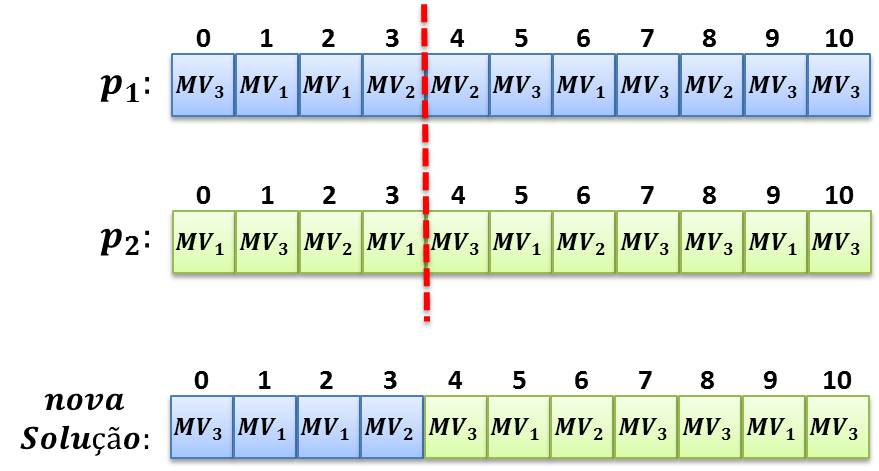
\includegraphics[width=1\linewidth]{figure/crossover1.jpg}
  \caption{\textit{Crossover} realizado no \textit{vetor de alocaçã}o.}
  \label{fig:crossover1}
  \vspace{2\baselineskip}
\end{subfigure}
\begin{subfigure}{.6\textwidth}
  \centering
  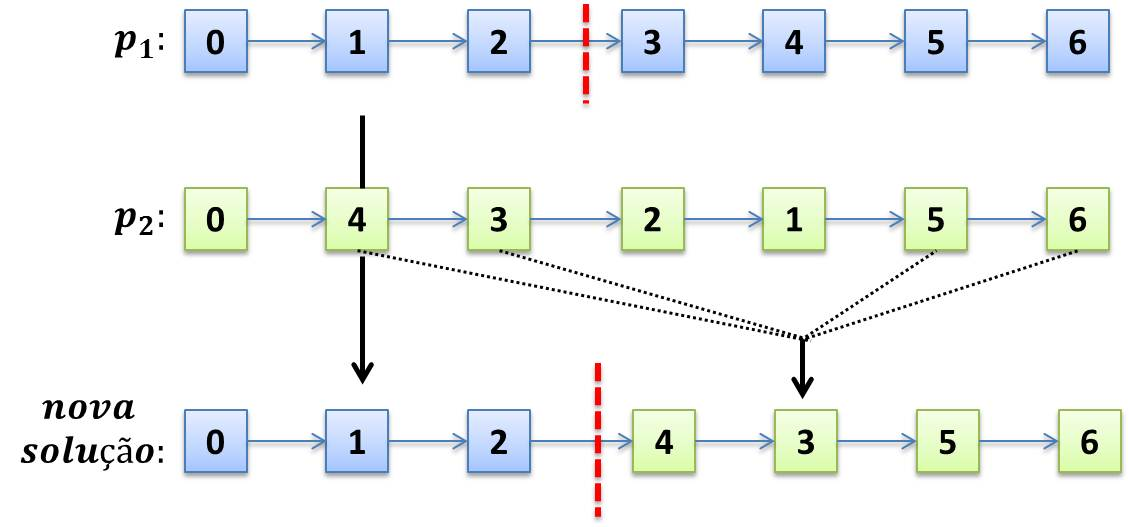
\includegraphics[width=1\linewidth]{figure/crossover2.jpg}
  \caption{\textit{Crossover} realizado na \textit{lista de execução}.}
  \label{fig:crossover2}
\end{subfigure}
\caption{Representação dos operadores de \textit{crossover} utilizados pelo AEH-ETAA.}
\label{fig:crossover}
\end{figure}


No caso do \textit{crossover} na \textit{lista de execução}, representado na Figura \ref{fig:crossover2} e presente nas linhas \ref{l:lista1} a \ref{l:lista2} do Algoritmo \ref{algo:crossover}, os genes do lado esquerdo do corte são copiados de $p_1$ para a solução filho (mantendo as mesmas posições). Já o restante dos genes da nova solução, são copiados da \textit{lista de execução} de $p_2$. Nesse último caso, as tarefas são verificadas uma a uma, e apenas as tarefas que ainda não estejam na solução filho são copiadas de $p_2$. Essa verificação é necessária para garantir que não haja repetição de tarefas, e assegurar que as ordens de precedência entre as tarefas sejam respeitadas.



\begin{algorithm}[H]
\caption{Procedimento \textit{Crossover}}\label{algo:crossover}

\begin{algorithmic}[1]
\Require Cromossomos $p1$ e $p2$.
\Ensure Novo Cromossomo (\textit{novo}).

    \State $corte1 \gets rand(1, |\textit{vetorAlocação}|)$\label{l:corte1}
    \State $corte2 \gets rand(1, |\textit{listaExecução}|)$\label{l:corte2}
    
    \For{$i \gets 1 \textbf{ a } |\textit{vetorAlocação}|$}
        \If{$i < corte1$}
            \State $novo.\textit{vetorAlocação}[i] \gets p1.\textit{vetorAlocação}[i]$
        \Else
            \State $novo.\textit{vetorAlocação}[i] \gets p2.\textit{vetorAlocação}[i]$        
        \EndIf
        
        \If{$i < corte2$} \label{l:lista1}
            \State $ novo.\textit{listaExecução} \gets novo.\textit{listaExecução} \cup p1.\textit{listaExecução}(i) $
        \EndIf
        
    \EndFor
    
    \For{$i \gets 1 \textbf{ a } |\textit{listaExecução}|$}
        \If{$p2.\textit{listaExecução}(i) \notin novo.\textit{listaExecução}$}            
            \State $ novo.\textit{listaExecução} \gets novo.\textit{listaExecução} \cup p2.\textit{listaExecução}(i) $
        \EndIf        
    \EndFor \label{l:lista2}

    
    \State \textbf{retorna} $novo$

\end{algorithmic}
\end{algorithm}

% Concerning the tasks execution order (Figure \ref{fig:crossover2}), genes from the left-hand side of the cut are copied from $parent_1$ to the genes of the same position of the offspring.
% The other genes of the offspring are obtained by checking each gene, in the same order they appear in $parent_2$, and copying it to the offspring whenever it has not been inserted in it yet. Thus, the precedence order of tasks is kept in the offspring.

Na fase de seleção (apresentada no Algoritmo \ref{algo:doPop}, linha \ref{l:selecaoInit} e \ref{l:selecaoFim}), os cromossomos da próxima população são selecionados a partir do conjunto chamado \textit{Soluções}, que é formado pelos novos cromossomos gerados e pela população anterior \textit{P}. Primeiro, para garantir que as melhores soluções sempre estarão incluídas na população, uma seleção elitista é aplicada na linha \ref{l:elitism}, na qual $5\%$ das melhores soluções são encontradas e adicionadas na próxima população \textit{P'}. Em seguida, as demais soluções são escolhidas utilizando o algoritmo de seleção por torneio e também são incluídas em \textit{P'}. Note que quando um cromossomo é selecionado ele é removido do conjunto \textit{Soluções} para prevenir que um mesmo cromossomo seja incluído mais de uma vez na população \textit{P'}.

\subsection{Operador de Mutação} \label{ssec:Mutation}

O operador de mutação é responsável pela diversificação da população, aumentando o espaço de busca e escapando dos chamados ótimos locais. Neste trabalho, o operador de mutação é executado apenas no \textit{vetor de alocação}. Os testes empíricos mostraram que a mutação aplicada à \textit{lista de execução} não apresenta melhorias significantivas em termos de qualidade da solução e, adicionalmente, aumenta o custo computacional do algoritmo.

 
A operação de mutação é chamada após o procedimento de \textit{crossover}, para cada nova solução gerada. Com base nas avaliações realizadas, fixou-se a probabilidade de mutação dos genes em $10\%$. Como pode ser visto na Figura \ref{fig:mutation}, o operador altera a identificação da MV aleatoriamente e, com isso, gera uma nova solução.
 
% The mutate operator is call for each new solution generated by the crossover procedure in the Algorithm \ref{algo:doPop}, on condition that each gene has a 10\% probability of being modified. As can be seen in Figure \ref{fig:mutation}, the VM identification \textit{Vm} is randomly changed. At the end, the fitness of the chromosome is recalculated and the new chromosome replaces the old one.


\begin{figure}[H]
	\center
  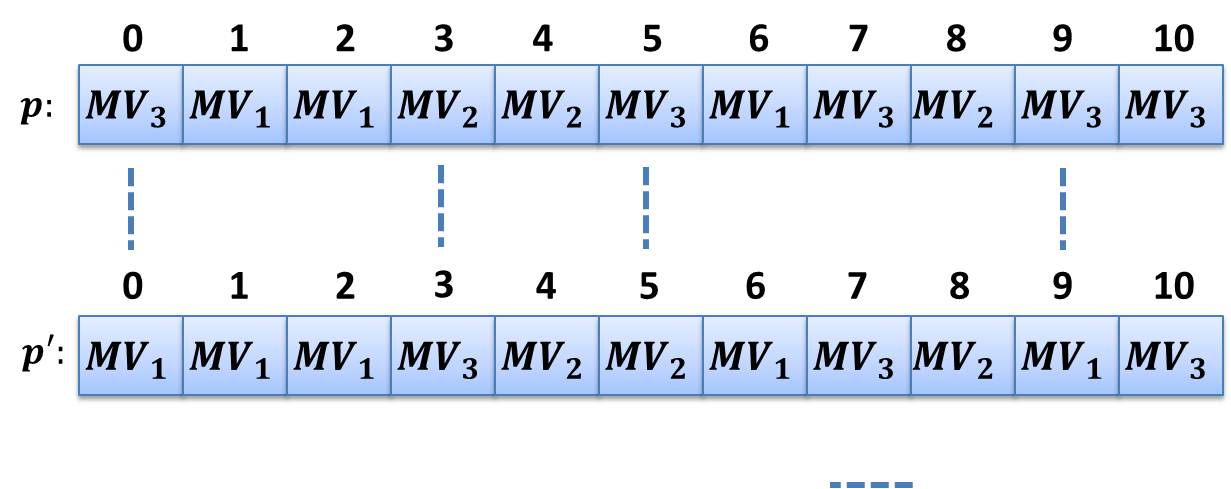
\includegraphics[width=0.6\linewidth]{figure/mutation.jpg}
  \caption{Operador de Mutação.}
  \label{fig:mutation}
\end{figure}

\subsection{Procedimentos de buscas locais} \label{ssec:localSearch}

Após a execução dos operadores de \textit{crossover} e mutação para construir a nova população, buscas locais são realizadas a $15\%$ das melhores soluções da população atual. As buscas locais ocorrem com uma probabilidade de $50\%.$ A porcentagem de soluções nas quais as buscas são realizadas e a probabilidade de ocorrência foram definidas através de testes empíricos feitos para ajustar os parâmetros do algoritmo. Como pode ser visto no Algoritmo \ref{algo:HEA} linha \ref{l:checkbl}, em cada iteração a probabilidade de busca local é verificada e, caso seja verdadeira, os procedimentos de buscas são executados.

Neste trabalho, três procedimentos de buscas locais foram definidos e são executados na seguinte ordem: (i) \textit{troca-mv} (Algoritmo \ref{algo:trocamv}), que executa a troca de dois elementos no \textit{vetor de alocação}; (ii) \textit{troca-posição} (Algoritmo \ref{algo:trocapos}), que troca a posição de dois elementos de mesma altura na \textit{lista de execução}; e (iii) \textit{move-elemento} (Algoritmo \ref{algo:moveelem}), que move uma tarefa ou um arquivo para uma MV diferente. Cada busca local é executada até que ocorra uma melhora na solução (primeira-melhora) ou até que todas as combinações sejam testadas.


\begin{algorithm}[H]
\caption{Procedimento \textit{troca-mv}}\label{algo:trocamv}

\begin{algorithmic}[1]
\Require Cromossomo $p$.
\Ensure Cromossomo $p$.
    
    \State $\textit{cópia} \gets p$
    
    \For{$i \gets 1 \textbf{ a } |\textit{vetorAlocação}|$}
        \For{$j \gets i + 1 \textbf{ a } |\textit{vetorAlocação}| $}
            \If{$p.\textit{vetorAlocação}[i] \neq p.\textit{vetorAlocação}[j]$}
                \State $troca(p.\textit{vetorAlocação}[i], p.\textit{vetorAlocação}[j])$
                \State $\textbf{calculaFitness}(p)$ \Comment{Algoritmo \ref{algo:fitness}.}
                \If{$ fitness(p) \textbf{ melhor que } fitness(\textit{cópia})$}
                    \State \textbf{retorna} $p$ 
                \Else
                    \State $troca(p.\textit{vetorAlocação}[i], p.\textit{vetorAlocação}[j])$ \Comment{Retorna ao estado anterior.}
                \EndIf                
            \EndIf
        \EndFor
    \EndFor    
    \State \textbf{retorna} \textit{cópia}
\end{algorithmic}
\end{algorithm}

\begin{algorithm}[H]
\caption{Procedimento \textit{troca-posição}}\label{algo:trocapos}

\begin{algorithmic}[1]
\Require Cromossomo $p$.
\Ensure Cromossomo $p$.
    
    \State $\textit{cópia} \gets p$
    
    \For{$i \gets 1 \textbf{ a } |\textit{listaExecução}|$}
        \State $tarefa_i \gets p.\textit{listaExecução}(i)$
        \For{$j \gets i + 1 \textbf{ a } |\textit{listaExecução}| $}
            \State $tarefa_j \gets p.\textit{listaExecução}(j)$
            \If{$altura(tarefa_i) = altura(tarefa_j)$}
                \State $troca(p.\textit{listaExecução}(i), p.\textit{listaExecução}(j))$
                \State $\textbf{calculaFitness}(p)$ \Comment{Algoritmo \ref{algo:fitness}.}
                \If{$ fitness(p) \textbf{ melhor que } fitness(\textit{cópia})$}
                    \State \textbf{retorna} $p$ 
                \Else
                    \State $troca(p.\textit{listaExecução}(i), p.\textit{listaExecução}(j))$ \Comment{Retorna ao estado anterior.}
                \EndIf                
            \Else
                \State \textbf{interrompe} \Comment{Interrompe laço e retorna ao laço externo.}
            \EndIf                
        \EndFor
    \EndFor    
    \State \textbf{retorna} \textit{cópia}
\end{algorithmic}
\end{algorithm}

\begin{algorithm}[H]
\caption{Procedimento \textit{move-elemento}}\label{algo:moveelem}

\begin{algorithmic}[1]
\Require Cromossomo $p$.
\Ensure Cromossomo $p$.
    
    \State $\textit{cópia} \gets p$
    
    \For{$i \gets 1 \textbf{ a } |\textit{vetorAlocação}|$}
        \State $\textit{MV\_atual} \gets p.\textit{vetorAlocação}[i]$
        \For{$\textit{MV\_prox} \gets  1 \textbf{ a } \textit{NÚMERO\_MVs} $}
            \If{$\textit{MV\_atual} \neq \textit{MV\_prox}$}
                \State $p.\textit{vetorAlocação}[i] = \textit{MV\_prox}$
                \State $\textbf{calculaFitness}(p)$ \Comment{Algoritmo \ref{algo:fitness}.}
                \If{$ fitness(p) \textbf{ melhor que } fitness(\textit{cópia})$}
                    \State \textbf{retorna} $p$ 
                \Else
                    \State $p.\textit{vetorAlocação}[i] = \textit{MV\_atual}$ \Comment{Retorna ao estado anterior.}
                \EndIf                
            \EndIf
        \EndFor
    \EndFor    
    \State \textbf{retorna} \textit{cópia}
\end{algorithmic}
\end{algorithm}


\begin{figure}[H]
\centering
\begin{subfigure}[t]{.5\textwidth}
  \centering
  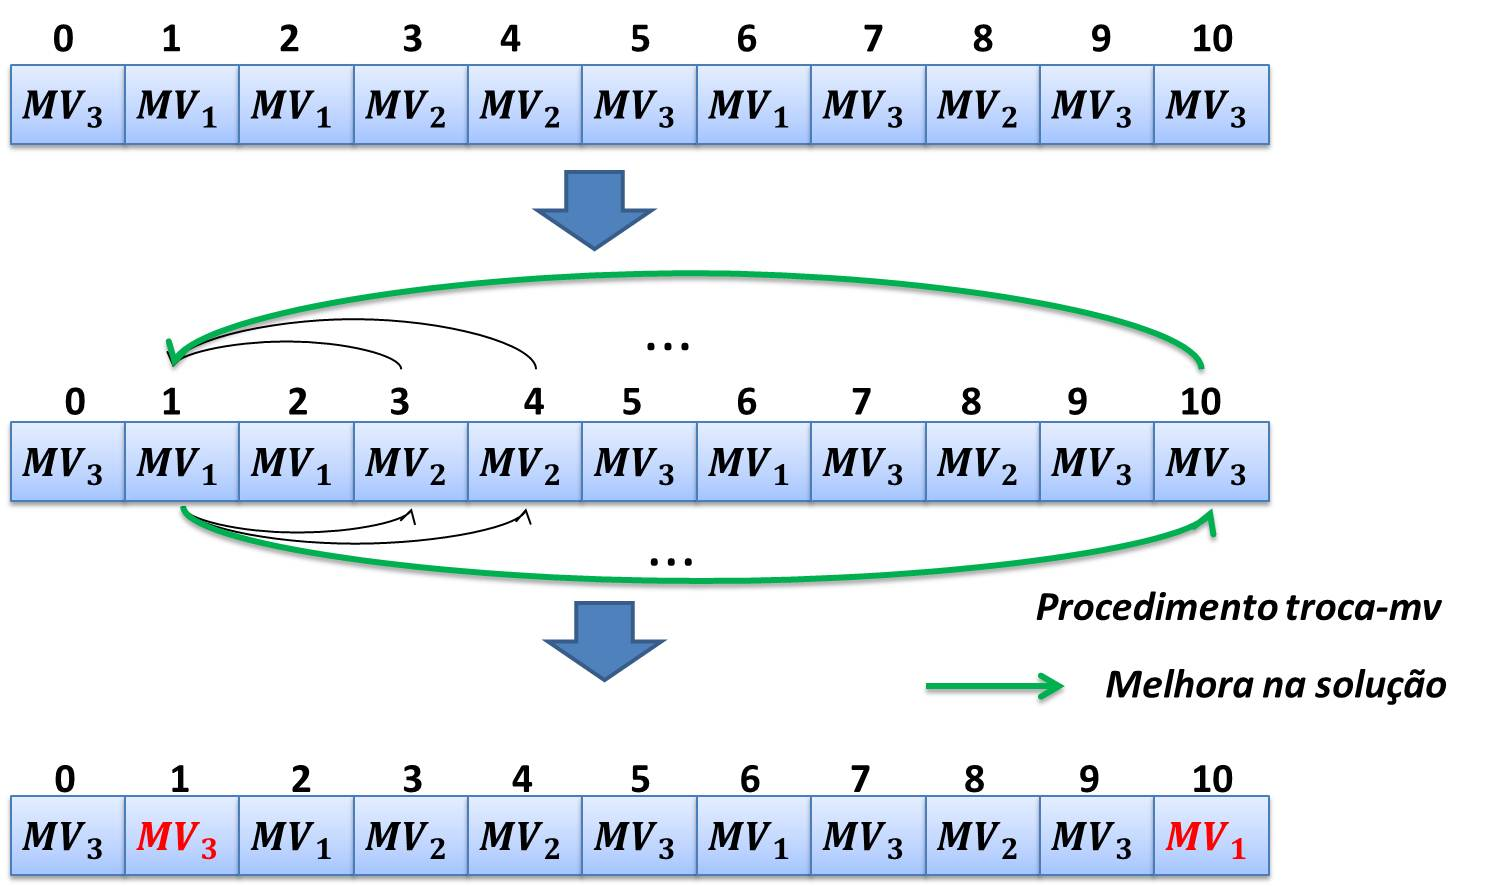
\includegraphics[width=1\linewidth]{figure/swap_vm.jpg}
  \caption{Troca de máquinas no \textit{vetor de alocação}.}
  \label{fig:swapvm}
\end{subfigure}%
\begin{subfigure}[t]{.5\textwidth}
  \centering
  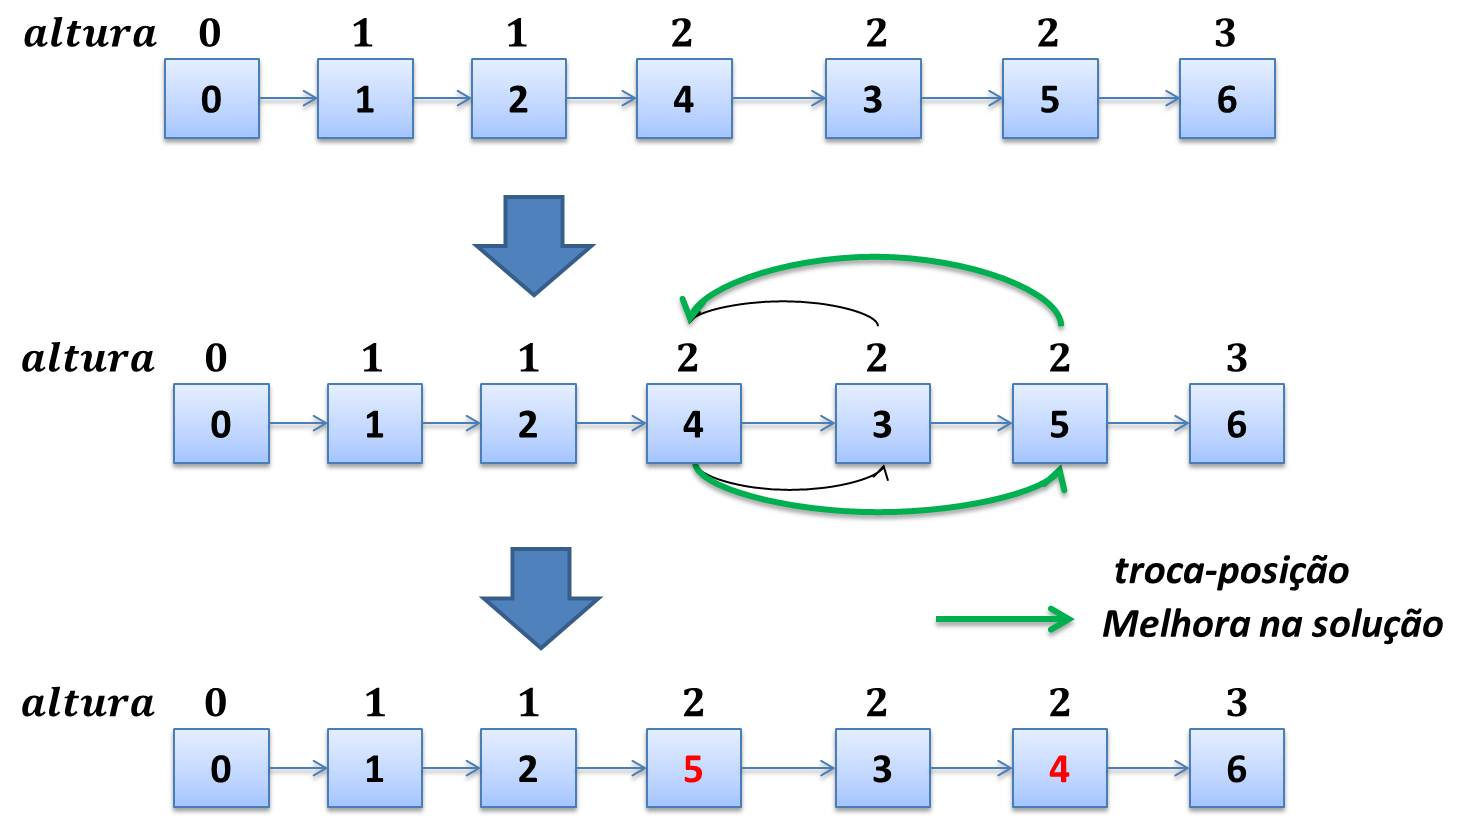
\includegraphics[width=1\linewidth]{figure/swap_sequence.jpg}
  \caption{Troca de tarefas na \textit{lista de execução}.}
  \label{fig:swapsequence}
\vspace{1\baselineskip}
\end{subfigure}
\begin{subfigure}{.5\textwidth}
  \centering
  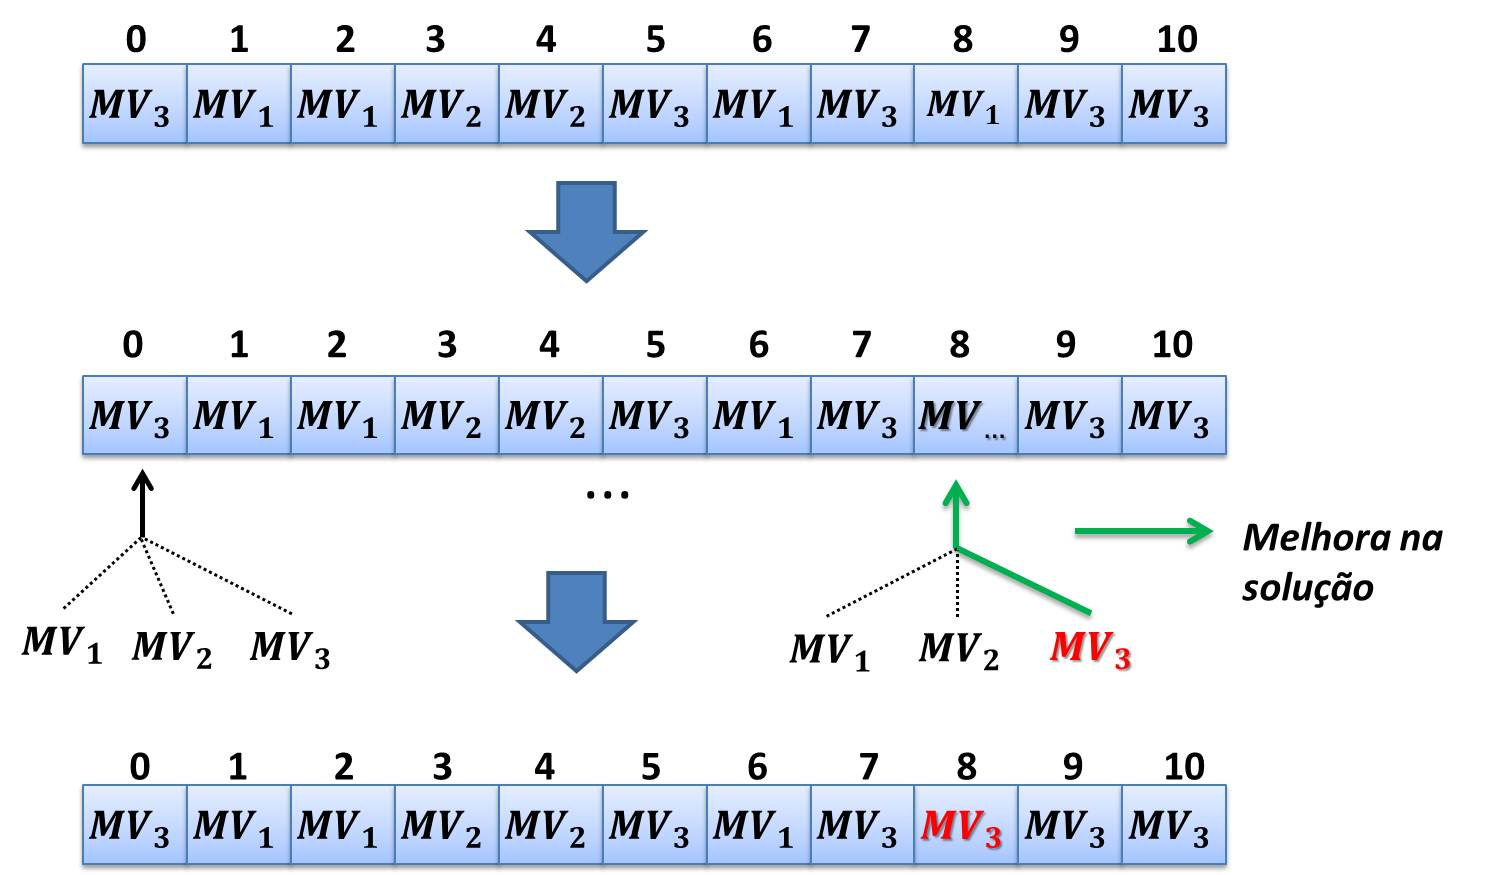
\includegraphics[width=1\linewidth]{figure/move_element.jpg}
  \caption{Move uma tarefa ou um arquivo de uma máquina para outra.}
  \label{fig:move}
\end{subfigure}
\caption{Procedimentos de Buscas Locais Implementados.}
\label{fig:localSearch}
\end{figure}



A Figura \ref{fig:localSearch} apresenta os três tipos de buscas locais utilizadas no AEH-ETAA. A Figura \ref{fig:swapvm} mostra a execução do procedimento \textit{troca-mv} que, após testar vários movimentos, troca os elementos da posição 1 e 10 do \textit{vetor de alocação}. A Figura \ref{fig:swapsequence} também executa várias trocas, até mover a ordem de execução da tarefa 4 e 5, que apresentam a mesma altura na \textit{lista de execução}. Por fim, na Figura \ref{fig:move}, a tarefa ou o arquivo é movido da $MV_2$ para $MV_3$.

\subsection{\textit{Path Relinking}}\label{ssec:pr}

\textit{Path relinking} é uma heurística capaz de gerar soluções intermediárias entre duas outras soluções. O operador começa com uma solução inicial e, passo a passo, insere elementos de uma solução guia. O objetivo é visitar novas soluções no caminho traçado entre uma solução e outra \cite{Glover2000}. Portanto, durante a execução do \textit{path relinking}, a distância entre as soluções diminui gradualmente.

% Path relinking is a heuristic capable of generating intermediate solutions between two other ones.
% It starts with an initial solution and, step by step, inserts elements of a target solution. Its goal is to visit new solutions in the path from one solution to another one \cite{Glover2000}.
% So, during the path relinking execution, the distance between the solutions diminishes gradually.

Neste trabalho, a distância de um cromossomo $p_i$ em relação a um cromossomo $p_j$ é dada pela soma do número de elementos (tarefas ou arquivos) alocados a diferentes MVs, com o número de movimentos necessários para que a \textit{lista de execução} de $p_i$ seja semelhante a de $p_j$. A Figura \ref{fig:distance} mostra a distância entre os cromossomos $p_1$ e $p_2$. Como pode ser visto, o número de tarefas e arquivos alocados em diferentes MVs é $5$ e apenas um movimento é necessário na \textit{lista de execução}, portanto $dist(p_1, p_2) = 6$.

% In the context of TaSDAP, the distance between a chromosome $chr_1$ and another $chr_2$ is the number of tasks and data files assigned to different VMs plus the number of swaps necessary to turn their task order lists exactly the same. Figure \ref{fig:distance} shows the distance of  chromosomes  $chr_1$ and $chr_2$.  The  number of tasks or data files placed in different VMs is five and the number of necessary swaps is one, so $dist(chr_1, chr_2) = 6$.

%\begin{figure}[H]
%	\center
%  \includegraphics[width=70mm,scale=0.9]{figure/distance.jpg}
%  \caption{Distance $dist(chr_1, chr_2) = 6$}
%  \label{fig:distance}
%\end{figure}

\begin{figure}[H]
\centering
\begin{subfigure}{.5\textwidth}
  \centering
  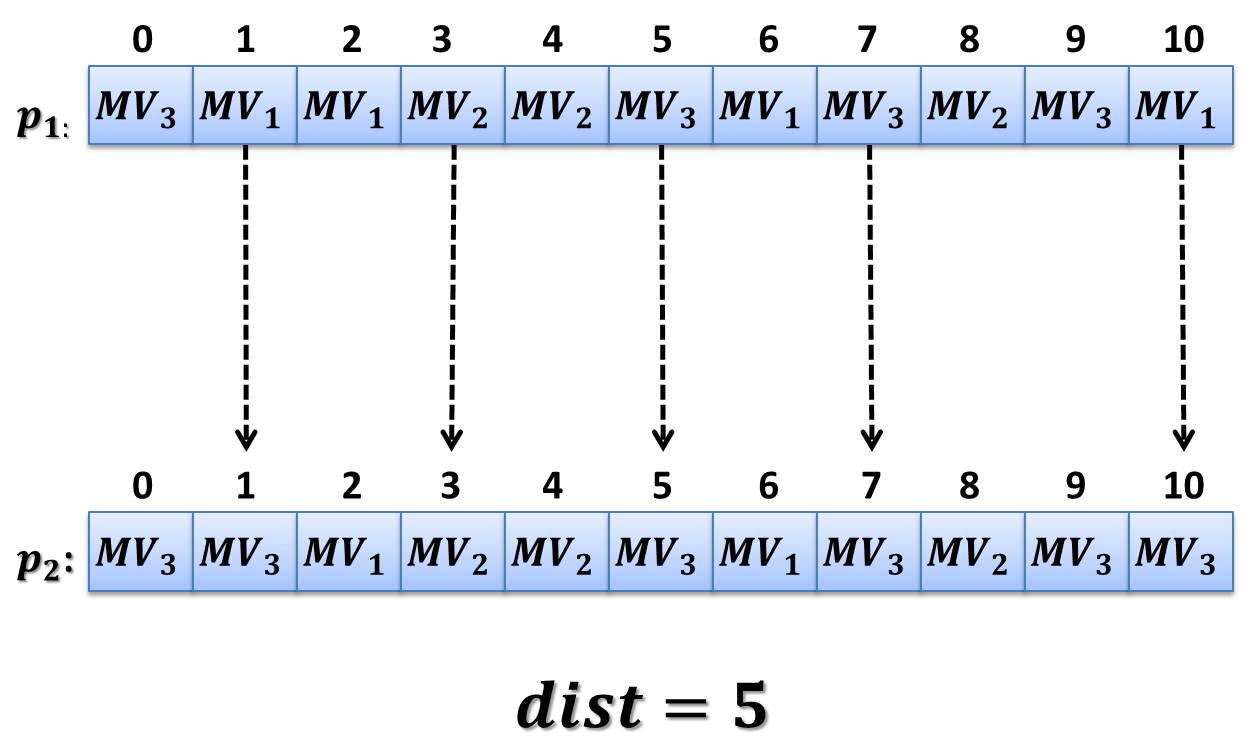
\includegraphics[width=.9\linewidth]{figure/distance1.jpg}
 \end{subfigure}%
\begin{subfigure}{.4\textwidth}
  \centering
  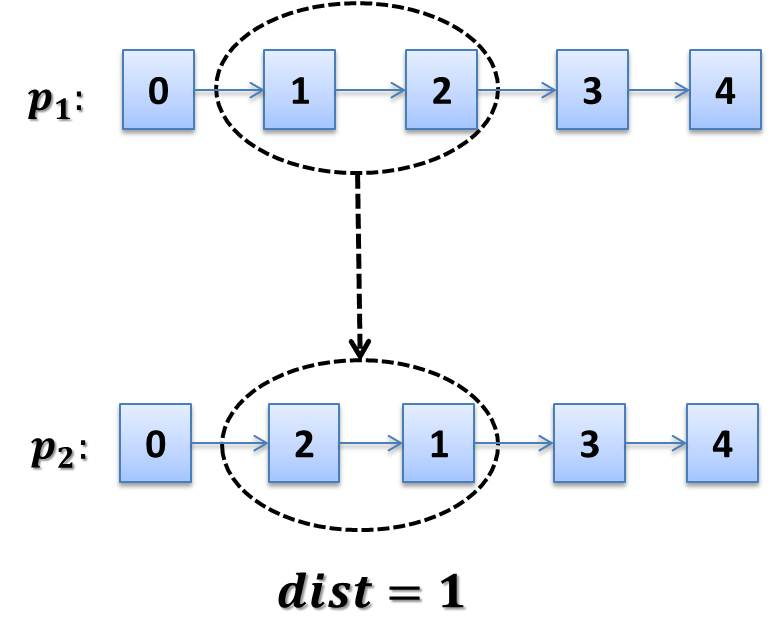
\includegraphics[width=.9\linewidth]{figure/distance2.jpg}
\end{subfigure}
\caption{Cálculo da distância entre os cromossomos $p_1$ e $p_2$, $dist(p_1, p_2) = 6$}
\label{fig:distance}
\end{figure}

O \textit{path relinking} é aplicado quando uma melhor solução (\textit{best}) é encontrada no procedimento principal (Algoritmo \ref{algo:HEA}, linha \ref{l:path1}). Como pode ser visto no Algoritmo \ref{algo:pr}, as soluções presentes no conjunto elite atuam como pontos iniciais da busca (chamados de \textit{origem}). O conjunto elite é composto pelas melhores soluções cuja distância entre cada uma delas é maior que $\alpha$, onde $\alpha$ é calculado como $25\%$ do número de tarefas e arquivos do \textit{workflow}. Esse parâmetro controla a diversidade do conjunto e, consequentemente, a eficiência da busca. Além disso, para controlar o número de buscas efetuadas, um limite máximo de $\beta$ cromossomos é definido para o conjunto elite, sendo que o valor de  $\beta$ é igual a metade do tamanho da população. Quando esse limite é alcançado, uma política de substituição \textit{First-in First-out} (FIFO) é aplicada para substituir a solução mais antiga pela mais nova. 
 
 \begin{algorithm}
 \caption{Procedimento \textit{PathRelinking}}\label{algo:pr}
 
 \begin{algorithmic}[1]
\Require Cromossomo $destino$ e Conjunto Elite $ConjElite$.
\Ensure Melhor cromossomo encontrado ($best$).
    
    \State $best \gets destino$
    
    \For{$cont \gets 1 \textbf{ a } |\textit{ConjElite}|$}
    
        \State $\textit{origem} \gets ConjElite(cont)$
                
        \For{$i \gets 1 \textbf{ a } |origem.\textit{vetorAlocação}|$} \label{l:prlaco}
            \If{$origem.\textit{vetorAlocação}[i] \neq destino.\textit{vetorAlocação}[i]$}
                \State $origem.\textit{vetorAlocação}[i] \gets destino.\textit{vetorAlocação}[i]$
                \State $\textbf{calculaFitness}(origem)$ \Comment{Algoritmo \ref{algo:fitness}.}
                \If{$fitness(origem) \textbf{ melhor que } fitness(best)$}
                    \State $best \gets origem$ \label{l:updatebest}
                \EndIf  
            \EndIf
        
        \EndFor
        
    \EndFor    
    \State \textbf{ retorna } $best$
\end{algorithmic}
\end{algorithm}


Como visto no Algoritmo \ref{algo:pr}, a busca se concentra no \textit{vetor de alocação} das soluções. A cada iteração do algoritmo (linha \ref{l:prlaco}), um elemento do \textit{vetor de alocação} da solução \textit{destino} é copiado para o vetor da solução origem. Na sequencia, o valor de \textit{fitness} da solução resultante é comparado com o melhor resultado obtido (armazenado em \textit{best}) e, caso o valor seja melhor, o \textit{best} é atualizado (linha \ref{l:updatebest}). Essas etapas são repetidas para cada um dos cromossomos do conjunto elite e, por fim, a melhor solução encontrada é retornada para o procedimento principal.
 
\subsection{Heurística \textit{move-arquivos}} \label{ssec:heuristic}

Quando um novo cromossomo é gerado sua viabilidade é avaliada. Se os arquivos alocados a uma MV excedem sua capacidade de armazenamento, a MV é considerada sobrecarregada e a heurística \textit{move-arquivos} é executada.

% When a new chromosome is generated, its feasibility is evaluated. If the data files assigned to a VM exceed its storage capacity, the VM is considered overloaded and the heuristic \textit{Move-file} is executed.

A heurística contém as seguintes etapas:
\begin{enumerate}
\item Seleciona a MV mais sobrecarregada, $MV_s$.
\item Selecione a MV com maior quantidade de espaço livre, $MV_d$.
\item Move o arquivo de menor tamanho alocado em $MV_s$ para $MV_d$.
\end{enumerate}

% The heuristic \textit{Move-file} contains the following steps: 
% \begin{enumerate}
% \item  Select the most overloaded VM, $m_s$.
% \item  Select the most underloaded VM, $m_d$.
% \item  Move the smallest size data file from VM $m_s$ to $m_d$.
% \end{enumerate}

Os passos acima são repetidos até que não haja MVs sobrecarregadas.

% The above  steps are repeated until there is no overloaded VM.

Baseado na hipótese de que as alocações definidas pela metaheurística correspondem as melhores alocações possíveis, parece razoável não modificar muito o cromossomo original, já que isso pode impactar o \textit{makespan} resultante. Para minimizar esse provável impacto, os arquivos de menor tamanho são selecionados para serem movidos.

% Based on the hypothesis that the assignments defined by the metaheuristic correspond to the best ones, it seems interesting not changing the original chromosome very much, since it could impact negatively on the makespan. In order to soften this probable impact, the smallest data files are selected to be moved.

\subsection{Função de \textit{fitness}} \label{ssec:fitness}

A função de \textit{fitness} pode ser definida como $f: s \rightarrow Z$, onde $s$ é uma solução viável do espaço de busca e $Z$ é um número inteiro que quantifica a qualidade da solução representada pelo cromossomo. Portanto, a função de \textit{fitness} permite ordenar as soluções em termos de qualidade e direcionar a busca para as melhores soluções \cite{Talbi2009}.

% Let $f: s \rightarrow Z$ be a fitness function, where $s$ is a feasible solution in the search space and $Z$ is an integer number that quantifies the quality of a solution represented by a chromosome. So, the fitness function allows for ordering the solutions in terms of quality and to direct the search towards the best solutions \cite{Talbi2009}.

Neste trabalho, a qualidade de um indivíduo é dada pelo \textit{makespan}, \textit{i.e.}, seja $p_i$ e $p_j$ dois cromossomos, se $makespan(p_i) < makespan(p_j)$, então a solução dado por $p_i$ é melhor que a dada por $p_j$. Ou seja, a função de \textit{fitness} se resume ao cálculo do \textit{makespan} associado a cada solução. O Algoritmo \ref{algo:fitness} efetua esse cálculo. Como pode ser visto, as informações da \textit{lista de execução} e do \textit{vetor de alocação} são utilizadas para estimar o tempo final de cada tarefa.

% In TaSDAP, the quality of an individual is given by the makespan, \textit{i.e.}, let $chr_i$ and $chr_j$ be two chromosomes, if $makespan(chr_i) < makespan(chr_j)$, then the solution given by $chr_i$ is better than the one given by $chr_j$. To calculate the makespan, we define the Algorithm \ref{algo:fitness}. As can be seen, the information in the structures \textit{order list} (sorting by the tasks height values) and \textit{assignment vector} are retrieved to compute the finish time of each task.  

\begin{algorithm}[H]
\caption{Procedimento \textit{CalculaFitness}}\label{algo:fitness}

\begin{algorithmic}[1]
\Require \textit{Vetor de Alocação} e \textit{Lista de Execução}.
\Ensure Valor do \textit{Makespan}.

    \State $Q \gets 0$ 
    \State $FT \gets 0$
    \For{$tf_i$ \textbf{em } $\textit{listaExecução} $}
        \State $MV_j \gets \textit{vetorAlocação}[tf_i]$
        \State $t\_max\_pred \gets maxTempoFinalPred(FT, tf_i)$
        \State $t\_inicial_i \gets \max{(t\_max\_pred, Q[MV_j])} $ \label{l:inicial}
        \State $t\_final_i \gets t\_inicial_i + \text{execução}(tf_i, MV_j) + leitura(tf_i) + escrita(tf_i)$ \label{l:final}
        \State $Q[vm_j] \gets t\_final_i$
        \State $FT[tf_i] \gets t\_final_i$
    \EndFor

    \State \textbf{retorna} $\max(FT)$ \label{l:fitretorno}


\end{algorithmic}
\end{algorithm}

No Algoritmo \ref{algo:fitness}, os vetores \textit{Q} e \textit{FT} são estruturas auxiliares usadas para manter o tempo calculado em cada etapa do algoritmo. O vetor \textit{Q} é indexado pelo identificador da máquina  e contém o tempo final da última tarefa executada na MV correspondente. Já o vetor \textit{FT} armazena o tempo final de cada tarefa $tf_i$, utilizada como índice do vetor.

% In Algorithm \ref{algo:fitness}, vectors \textit{Q} and \textit{FT} are auxiliary structures used to keep the times computed in every step of the algorithm.  Vector  \textit{Q}  is indexed by the VM identification ($m_j$) and  contains the finishing time of the last task executed in the corresponding VM. Each element of   vector \textit{FT}  corresponds to a $task_i$ and  contains the finishing time of  the associated task.

Os cálculos de tempo inicial e final de cada tarefa seguem o modelo apresentado na Subseção \ref{sec:problemDef}. Primeiramente, o tempo inicial da tarefa $tf_i$ é computado como o máximo entre os tempos finais de seus predecessores imediatos (representado por \textit{t\_max\_pred}) e o tempo final da ultima tarefa executada na $MV_j$ (armazenado em $Q[MV_j]$), como apresentado na linha \ref{l:inicial}.

% The calculations of the start and  finishing times  of each task follows the model presented in Subsection \ref{sec:problemDef}. Firstly, the start time of $task_i$  is  computed as the the maximum finishing time among all its  immediate predecessors (represented by  \textit{max\_pred\_time}) and the finishing time of the last task executed in VM $m_j$ (stored in $Q[m_j]$), as presented in line 6. 

Em seguida, na linha \ref{l:final}, o tempo final da tarefa $tf_i$ é calculado como a soma dos seguintes valores: (i) o tempo inicial de $tf_i$ ($t\_inicial_i$); (ii) o tempo de execução de $tf_i$ quando executada na $MV_j$; (iii) o tempo necessário para ler todos os dados de entrada de $tf_i$; e (iv) o tempo necessário para escrever todos os arquivos gerados por $tf_i$. Finalmente, na linha \ref{l:fitretorno}, o algoritmo retorna o valor de \textit{makespan}.

% Then, in  line 7, the finishing time of $task_i$ is computed by summing the following values: (i) the start time of $task_i$ ($start\_time_i$); (ii) the execution time of $task_i$ when executed in VM $m_j$; (iii) the  necessary time for reading all required data files by  $task_i$; and (iv) the  necessary time  for writing all data files generated by $task_i$. Finally, in line 10, the algorithm returns the makespan that  is  the maximum finishing time among all tasks of the workflow.



\chapter{Resultados Experimentais}\label{chap6}


Esse capítulo apresenta os experimentos conduzidos com AEH-ETAA para avaliar a abordagem proposta. Foram conduzidos experimentos teóricos e práticos. As seções seguintes apresentam esses experimentos e discutem os resultados obtidos.
% This section presents experiments conducted with HEA-TaSDAP to evaluate the proposed approach. We conducted two types of experiments: theoretical and practical ones. The central idea of this section is to compare the proposed scheduling approach with existing solutions that can be used to schedule workflows in clouds. It is worth mentioning that all schedules used in this section for experiments and all optimization code are available in a BitBucket Git repository (\url{https://bitbucket.org/danielcmo/hea-tasdap}). 



\section{Experimentos Teóricos}

O AEH-ETAA foi comparado em termos de qualidade de solução  e tempo de execução com: (i) as soluções dadas pela formulação matemática IP-ETAA (resolvida com CPLEX $12.5.1$); (ii) A heurística MinMin \cite{minmin}; e (iii) a heurística HEFT \cite{HEFT}. As heurísticas MinMin e HEFT foram escolhidas pois executam em tempo polinomial, produzem escalonamentos eficientes e foram utilizados na comparação de diversos trabalhos relacionados \cite{Rahman2007, Lopez, Yu2006}.

% 	We firstly evaluate HEA-TaSDAP, in terms of  quality of solution and execution time, by comparing it with: (i) the solutions given by mathematical formulation TaSDAP-IP (solved with CPLEX $12.5.1$); (ii) the MinMin-Task Scheduling Heuristic (MinMin-TSH) \cite{MINMIN}; and (iii) the Heterogeneous Earliest Finish Time (HEFT) \cite{HEFT}.  We have chosen MinMin-TSH and HEFT because these heuristics run in polynomial time, produce efficient schedules and have been used as baselines in related works  \cite{Rahman2007,Lopez, Yu2006}. 
	
	
Os testes foram realizados em um computador com processador Intel Core i7-3770 CPU $3,40$ GHz com 12GB memoria, executando o Ubuntu $14.04$. O algoritmos AEH-ETAA, MinMin e HEFT foram implementados com C++, e compilados com o G++ versão $5.3.0$.

% 	Tests were run in a computer with a processor Intel Core i7-3770 CPU 3.40 GHz with 12Gb memory running Ubuntu $14.04$. The HEA-TaSDAP, MinMin-TSH and HEFT were implemented with C/C++, and compiled with g++ version $5.3.0$.
	
Nesses experimentos, foram utilizados dois tipos de instâncias sintéticas. O primeiro tipo, usado na comparação entre o AEH-ETAA e IP-ETAA (Subseção \ref{ssec:CompEX}), é composto por soluções geradas randomicamente, variando o número de tarefas, a quantidade de arquivos e o modelo de representação dos \textit{workflows}. O segundo, utilizado na Subseção \ref{ssec:compT}, foi gerado pelo \textit{Workflow Generator} \cite{Silva2014} (\url{https://confluence.pegasus.isi.edu/display/pagasus/WorkflowGenerator}), uma aplicação que gera \textit{workflows} sintéticos utilizados na avaliação de diversos algoritmos de escalonamento. O \textit{Workflow Generator} utiliza dados coletados de execuções reais de WfCs executados em \textit{grids} e ambientes de nuvem e, por conta disso, apresenta uma boa acurácia em relação às características reais dos \textit{workflows}.

% 	We use two types of synthetic instances in these experiments. The first one, used in the comparison  between HEA-TasDap and TaSDAP-IP (Subsection \ref{ssec:CompEX}), was randomly generated varying the number of tasks, data files and representations of workflows, as explained later. The second type, used in Subsection \ref{ssec:compT}, was generated by the Workflow Generator \cite{Silva2014}  (\url{https://confluence.pegasus.isi.edu/display/pegasus/WorkflowGenerator}). This application generates instances of workflow executions for evaluation of algorithms and systems on a range of workflow sizes. All data within these synthetic workflows is gathered from real executions of scientific workflows on the grid and in the cloud from the Pegasus' team in ISI @ University of Southern California.
	
A metaheurística AEH-ETAA foi executada com uma população de 50 indivíduos e o critério de parada foi definido como 100 iterações sem melhorias.

% 	The metaheuristic HEA-TaSDAP was executed with a population of 50 individuals and the stopping criterion was satisfied after 100 iterations without improvement. Concerning  the other parameters, the algorithm uses the ones defined in Section \ref{sec:HEA}.  It is worth mentioning that all parameters were adjusted empirically after several tests.
	


\subsection{Comparação do AEH-ETAA com a Abordagem Exata IP-ETAA}\label{ssec:CompEX}

O AEH-ETAA e o IP-ETAA foram avaliados utilizando um conjunto de 12 instâncias divididas em 4 grupos de acordo com o seus tamanhos. Para cada grupo, três instâncias diferentes foram geradas variando o número de tarefas, arquivos, e a representação do \textit{workflow}. Dois ambientes computacionais foram definidos para a simulação, com 3 e 5 MVs. O tamanho dos arquivos (MB) e tempo de execução das tarefas (segundos) foram definidos aleatoriamente entre 0,1 e 100. Uma capacidade de armazenamento de 10 GB foi definida e enlaces de 5, 10 e 15 MB/s foram utilizados. Por fim, o valor de \textit{slowdown} das máquinas foi configurado entre 0,01 e 1. A Tabela \ref{tabletoy} mostra a quantidade de tarefas e arquivos para cada instância gerada. Além disso, a estrutura básica do \textit{workflow} de cada uma delas é apresentada de acordo com a classificação feita por Bharathi \textit{at al.} \cite{Bharathi2008}. A Figura \ref{fig:structure} apresenta essa classificação e as estruturas dos \textit{workflows}.

% 	HEA-TaSDAP and TaSDAP-IP were evaluated using a set of 12 random instances divided into 4 groups according to their sizes. For each group, three different instances were generated by varying the number of tasks, files, and the representation of the workflow. Two computational environments were defined for simulation, with 3 and 5 VMs. File sizes (MB) and the process execution time (seconds) were randomly set between 0.1 and 100. The storage capacity of 1TB has been set, and the transfer link rates were 5, 10 and 15 MB/s. Finally, the slowdown of the machines were set between 0.01 and 1. Table \ref{tabletoy} shows the amounts of tasks and files for each generated instance. In addition, the basic workflow structures found on them are presented according to the classification made by Bharathi \textit{et al.} \cite{Bharathi2008}.

\begin{table}[!ht]

    \begin{center}
        \caption{Descrição das Instâncias Utilizadas na comparação com a formulação matemática.}
        \label{tabletoy}
        
         \begin{tabular}{|c |c |c |c |}
            \hline
            \textbf{\textbf{Referência}} & \textbf{Estrut. Básica} & \textbf{Núm. tarefas} & \textbf{Núm. arquivos}\\
            \hline\hline
                5A           & Processamento                            & 2     & 3\\
                5B           & Processamento e agregação de dados       & 2     & 3\\
                5C           & Agregação de dados                       & 1     & 4\\
                \hline
                7A          &   Agregação e redistribuição de dados     & 2     & 5\\ 
                7B          &   Processamento                           & 3     & 4\\
                7C          &   Agregação de dados e \textit{pipeline}  & 3     & 4\\
                \hline
                10A         & Agregação de dados                        & 4  & 6\\
                10B         & Redistribuição de dados                   & 3  & 7\\
                10C         & Distribuição de dados e \textit{pipeline} & 3  & 6\\
                \hline
                15A         & Agregação e distribuição de dados         & 5  & 10\\
                15B         & Distribuição de dados e \textit{pipeline} & 4  & 11\\
                15C         & Agregação e distribuição de dados         & 5  & 10\\                  
             \hline
         \end{tabular}
    \end{center}
\end{table}


\begin{figure}[H]
\centering
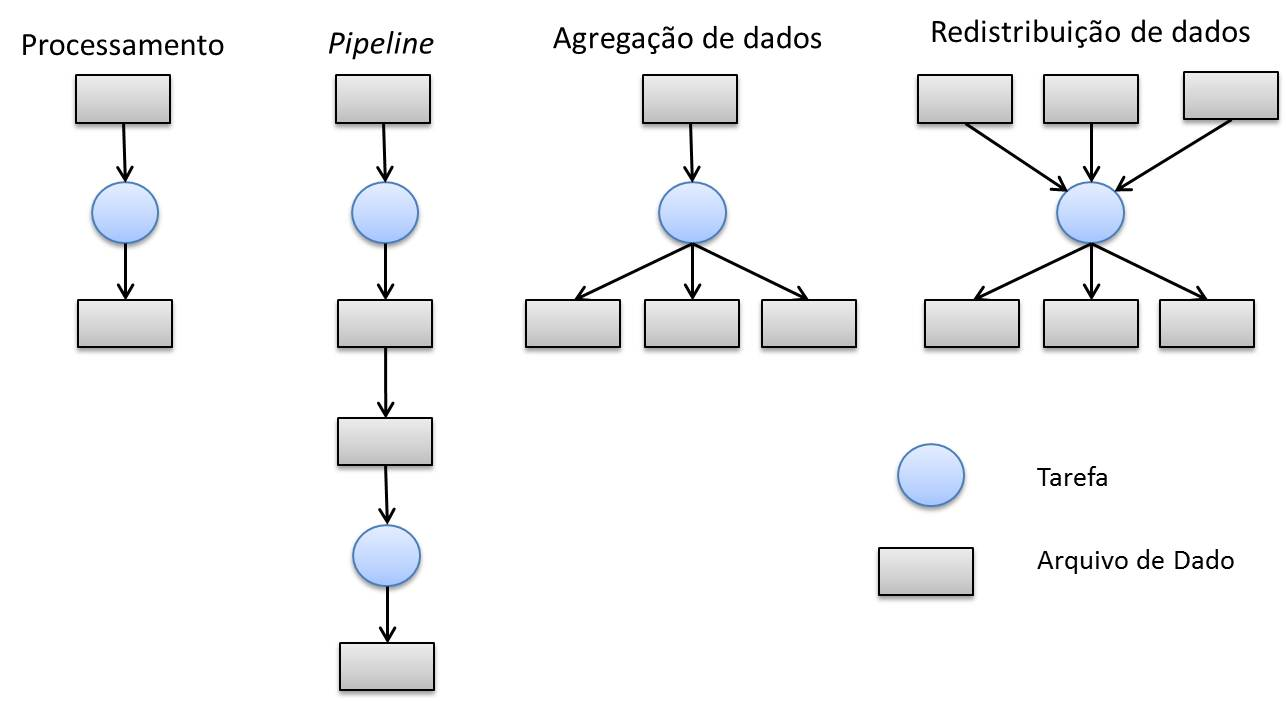
\includegraphics[width=.6\linewidth]{figure/structure.jpg}
\caption{Estruturas básicas dos \textit{workflows} (adaptado de \cite{Bharathi2008}).}
\label{fig:structure}
\end{figure}


	 
A Tabela \ref{teorico} apresenta os resultados obtidos pela abordagem exata e pela metaheurística AEH-ETAA. A primeira coluna identifica as instâncias e nas duas colunas seguintes são apresentados os resultados obtidos pelo AEH-ETAA: \textit{makespan} obtido e tempo de execução do algoritmo. Em seguida, nas duas próximas colunas, são apresentadas as informações referentes a abordagem exata. Por fim, a diferença percentual entre a solução dada pela metaheurística e pela abordagem exata é mostrada. O valor de \textit{makespan} apresentados para AEH-ETAA representam a média de cinco execuções. Além disso,  como os valores de desvio padrão foram iguais a zero para quase todas as instâncias,  com exceção das instâncias $15B\_m3, 15B\_m5$ e $15A\_m5$ que foram menos de $0,6\%$, essa informação não é apresentada.
	 
% 	 Table \ref{teorico} summarizes the results obtained by exact approach and the HEA-TaSDAP metaheuristic. The first column identifies the instance. The following two columns present the results obtained by HEA-TaSDAP: makespan and the execution time to obtain the solution. Following, the next 2 columns present the same results for the exact approach. Finally, the last column, shows the gap between the solutions given by HEA-TaSDAP and the exact approach (mathematical formulation). The values shown for HEA-TaSDAP are averages of five executions. The standard deviations were zero for almost all instances, except $15B\_m3$, $15B\_m5$ and $15A\_m5$, which were less than $0.6$. 


Analisando a Tabela \ref{teorico} pode-se observar que para todas as instâncias avaliadas o AEH-ETAA obteve soluções com uma diferença percentual baixa (média $1,1\%$), com tempos de execução  significativamente menores em relação à formulação matemática resolvida com o CPLEX, em média $1,5$s contra $12.640,3$s, respectivamente. Além disso, o CPLEX não foi capaz de encontrar soluções viáveis para as instancias $10A\_m5$ e $15C\_m5$ dentro de um limite de 24 horas.
Ademais, na instância $15C\_m3$, o CPLEX não foi capaz de encontrar a soluções ótima. Embora esses resultados sejam encorajadores, o AEH-ETAA também foi avaliado com outras heurísticas utilizando outras instâncias, como apresentado nas próximas seções.
	 
\begin{table}[H]
\begin{minipage}{\textwidth}   
    \begin{center}
            \caption{Resultados da metaheurística AEH-ETAA e da formulação matemática utilizando o CPLEX.}
        \label{teorico}        
          \begin{tabular}{|c|r|r|r|r|r|}
            \hline
            \multirow{1}{*}{\textbf{Instâncias}} & \multicolumn{2}{|c|}{\textbf{AEH-ETAA}} & \multicolumn{2}{|c|}{\textbf{Formulação Matemática}} & \multirow{1}{*}{\textbf{Dif. Percentual}}\\
\cline{2-5}
            \hline\hline          
5A\_m3	&	10,0	&	0,83    &	10,0	&	 4,2    &	0,0	\\
5B\_m3	&	11,0	&	0,79    &	11,0	&	 14,0   &	0,0	\\
5C\_m3	&	13,0	&	0,71    &	13,0	&	 2,8    &	0,0	\\
7A\_m3	&	21,0	&	0,96    &	21,0	&	140,8	&	0,0	\\
7B\_m3	&	16,0	&	1,17    &	16,0	&	 7,3	&	0,0	\\
7C\_m3	&	14,0	&	1,11	&	14,0	&	105,0	&	0,0	\\
10A\_m3	&	21,0	&	1,80	&	21,0	&	1644,6	&	0,0	\\
10B\_m3	&	12,0	&	1,74	&	12,0	&	21,4	&	0,0	\\
10C\_m3	&	21,0	&	1,22	&	21,0	&	316,7	&	0,0	\\
15A\_m3	&	16,0	&	2,47	&	16,0	&	2606,6	&	0,0	\\
15B\_m3	&	11,4	&	3,01	&	11,0	&	600,9	&	3,6	\\
15C\_m3\footnote{\label{1footnote} O CPLEX não foi capaz de encontrar solução viável para a instância.}&	19,2	&	2,42	&	94,0	&	86395,5	&	\textbf{--}	\\
5A\_m5	&	10,0	&	0,90	&	10,0	&	14,4	&	0,0	\\
5B\_m5	&	 9,0	&	0,50	&	 9,0	&	462,6	&	0,0	\\
5C\_m5	&	10,0	&	0,75	&	10,0	&	 9,0	&	0,0	\\
7A\_m5	&	27,0	&	0,97	&	27,0	&	1836,4	&	0,0	\\
7B\_m5	&	26,0	&	1,26	&	26,0	&	21,0	&	0,0	\\
7C\_m5	&	16,0	&	1,09	&	16,0	&	2426,9	&	0,0	\\
10A\_m5\footref{1footnote}&	25,0	&	1,58	&	\textbf{--}	    &	86489,2	&	\textbf{--}	\\
10B\_m5	&	14,0	&	1,75	&	13,0	&	103,0	&	7,6	\\
10C\_m5	&	47,6	&	1,88	&	47,0	&	7353,5	&	1,2	\\
15A\_m5	&	16,0	&	2,64	&	16,0	&	15783,9	&	0,0	\\
15B\_m5	&	11,0	&	2,97	&	10,0	&	10764,3	&	10,0	\\
15C\_m5\footref{1footnote}&	20,0	&	2,49	&	\textbf{--}	    &	86243,0 &  \textbf{--}	\\
\hline
Média	&	17,4	&	1,5	    &	20,2	&	12640,3	&	1,1	\\
             \hline
         \end{tabular}
    \end{center}
    \end{minipage}
\end{table}
	 
	 

\subsection{Comparação do AEH-ETAA com as Heurísticas  HEFT e MinMin}\label{ssec:compT}

Para comparar a performance e a qualidade dos resultados do AEH-ETAA com as heurísticas HEFT e MinMin, as instâncias sintéticas produzidas pelo \textit{workflow generator} baseadas nos \textit{workflows} Montage, Cybershake, Epigenomics e Inpiral  \cite{juve2406180} foram escolhidas. Cada instância tem as seguintes informações: (i) um DAG representando o \textit{workflow}; (ii) o tempo de execução de cada tarefa em relação a uma máquina com capacidade de processamento conhecida; e (iii) o tamanho de cada arquivo de entrada e de saída. A Tabela \ref{workflowCharacteristics} apresenta um resumo das principais características de cada um destes \textit{workflows}. Para o ambiente de execução, foram consideradas as características (largura de banda, capacidade de armazenamento e processamento) das MVs oferecidas pela Amazon EC2. Foram utilizadas 4 MVs: 1 m3.medium (1 vCPU Intel Xeon E5-2670 v2); 1 m3.large (2 vCPU Intel Xeon E5-2670 v2); 1 m3.xlarge (4 vCPU Intel Xeon E5-2670 v2); 1 m3.2xlarge (2 vCPU Intel Xeon E5-2670 v2). Portanto, embora a avaliação seja teórica, os dados utilizados na descrição dos \textit{workflows} e das MVs foram adquiridos com base em cenários reais. 


% In order to compare the performance and the quality of the results of  HEA-TaSDAP, HEFT and  MinMin-TSH, the aforementioned synthetic  workflows  produced by workflow generator: Montage, Cybershake, Epigenomics and Inspiral workflows \cite{Juve2406180} were chosen.  Each instance (workflow) has the following corresponding information: (i) a Direct Acyclic Graph representing  tasks  and data files of the workflow; (ii) execution time  of each task in a machine with known processing capacity; and (iii) size of each  input and output data file.   Table \ref{workflowCharacteristics} shows the main characteristics of each workflow.

\begin{table}[!ht]
    \begin{center}
        \caption{Atributos dos \textit{workflows} utilizados na avaliação teórica entre o AEH-ETAA, HEFT e MinMin (Adaptado de \cite{Szabo2013}).}
        \label{workflowCharacteristics}
        
         \begin{tabular}{|c |c |c |c |}
            \hline
            \multirow{2}{*}{\textbf{Workflow}} & \multirow{1}{*}{\textbf{Tipo}} & \textbf{Núm. de tarefas} & \textbf{Núm. de arquivos}\\
            & \textit{ I/O; Memória; CPU}    &\textbf{por instâncias}& \textbf{dinâmicos e estáticos}\\
            \hline\hline
    Cybershake  & Baixo; Baixo; Médio     & 30; 50; 100            & 49; 79; 154 \\
	Epigenomics & Baixo; Médio; Alto      & 24; 47; 79; 100; 127   & 38; 71; 119; 152; 192;  \\
	Montage	    & Alto; Baixo; Baixo      & 25; 50; 100            & 38; 53; 93 \\
	Inspiral    & Baixo; Médio; Alto      & 30; 50; 100            & 47; 77; 151  \\
             \hline
         \end{tabular}
    \end{center}
\end{table}




% We also considered the characteristics of the VMs from Amazon EC2 cloud environment. So, although we are theoretically evaluating the algorithms, the used data (structure of workflows and VMs characteristics) were acquired from real scenarios. The used cloud environment is composed by 4 VMs: 1 m3.medium (1 vCPU Intel Xeon E5-2670 v2); 1 m3.large (2 vCPU  Intel Xeon E5-2670 v2); 1 m3.xlarge (4 vCPU Intel Xeon E5-2670 v2); 1 m3.2xlarge (8 vCPU Intel Xeon E5-2670 v2).  We also considered the following information about  each VM: (i) network bandwidth; (ii) storage capacity; and (iii) processing capacity. 

O tempo de execução das tarefas é definido como o produto do \textit{tempo base} pelo valor de \textit{slowdown} da MV que executará a tarefa. O valor de \textit{slowdown} é definido como $\frac{P_B}{P_{mv_{j}}}$, onde $P_B$ é a capacidade de processamento da máquina usada na estimativa do \textit{tempo base}, e $P_{mv_{j}}$ é a capacidade de processamento da máquina virtual $mv_j$ usada no experimento. Portanto, o \textit{slowdown} dá a variação da capacidade de processamento de uma MV em relação a máquina utilizada para calcular o \textit{tempo base} da tarefa. Neste experimentos, o \textit{tempo base} e a capacidade do processamento da máquina $P_B$ foram obtidos a partir das instâncias dadas pelo \textit{Workflow Generator}, enquanto $P_{mv_{j}}$ é a capacidade de processamento da máquina virtual oferecido pela Amazon EC2.

% It is worth mentioning that the execution time of a task is defined as the product between a basis time and the machine slowdown where it will be executed. A machine slowdown is defined  as  $\frac{P_B}{P_{m_{j}}}$, where $P_B$ is the  processing capacity of the machine  used to calculate the basis time, and   $P_{m_{j}}$  is the  processing capacity of the virtual machine of our experiment. So,  the  slowdown represents the processing capacity of a virtual machine when compared with the  machine used to calculate the basis time.  In our experiments, the basis time and the processing capacity $P_B$  were obtained from  instances of the Workflow Generator, while $P_{m_{j}}$  is the  processing capacity of the virtual machine  from  Amazon EC2. The parameter of transfer rate was estimated through practical experiments using the tool Iperf, available in \url{https://iperf.fr}.

A Tabela \ref{teoricoSintetico} apresenta o \textit{makespan} obtido pela média de 5 execuções, o desvio padrão relativo (RSD) e o tempo de execução do AEH-ETAA. Também são apresentados o \textit{makespan} obtido com as heurísticas MinMin e HEFT. Como essas heurísticas são determinísticas, os resultados sempre serão os mesmos para entradas semelhantes, os valores de \textit{makespan} não são médias de execuções e sim o valor obtido com uma única execução. Além disso, o tempo de execução do MinMin e do HEFT não são apresentados, pois eles são insignificantes (menos que 1 minuto).


Como pode ser visto na Tabela \ref{teoricoSintetico} a metaheurística AEH-ETAA supera ambos os algoritmos comparados. De fato, esses resultados são esperados, já que variações das soluções dadas pelo MinMin e pelo HEFT são utilizadas pela metaheurística na geração da população inicial. Porém, vale notar que houve uma melhora na qualidade dos valores de \textit{makespan} em todos os casos de teste, com um tempo de execução aceitável (menos de 9 minutos no pior caso). O AEH-ETAA apresentou uma melhora média de $22,72\%$ em relação ao MinMin e $11,15\%$ em relação ao HEFT.

% Table \ref{teoricoSintetico} presents the makespan (the average of 5 executions), Relative Standard Deviation (RSD) and the execution time of HEA-TaSDAP. It also presents the makespan of MinMin-TSH and HEFT, and since they are deterministic heuristics, the result is always the same for each execution of the algorithm. The execution times of MinMin-TSH and HEFT are not presented, since they are negligible (less than 1 minute). Note that, HEA-TaSDAP outperforms both MinMin-TSH and HEFT algorithms.

% In fact, these results were already expected, since variations of solutions given by MinMin-TSH and HEFT are used in initial population. It worth noticing that with our proposal we improved the quality of the makespan in all cases and with a acceptable run time (less than 9 minutes in the worst case). The HEA-TaSDAP showed an average improvement of 22.72\% in relation of MinMin-TSH and 11.15\% in relation of HEFT.


\begin{table}[H]
\small
\begin{center}
\caption{Resultados da comparação entre AEH-ETAA, HEFT e MinMin.}
\label{teoricoSintetico}
\begin{tabular}{|c|r|r|r|r|r|}\hline 
\multirow{2}{1cm}{\textbf{Inst}.} & \multicolumn{1}{|c|}{\textbf{MinMin}} & \multicolumn{1}{|c|}{\textbf{HEFT}} & \multicolumn{3}{|c|}{\textbf{AEH-ETAA}} \\    
\cline{2-6}  
                &\textit{	Makesp. (min)} & \textit{Makesp. (min)} &	\textit{Makesp. (min)} & \textit{RSD}	 & \textit{Exec. (min)}\\
\hline
\hline
Cybershake30    &	11,98	       & 11,28          &   10,25              & 0,0019    &	0,39          \\
Cybershake50    &	14,88	       & 16,65	        &   12,46	       & 0,0264    &	2,19          \\
Cybershake100   &   26,93	       & 28,08	        &   14,52	       & 0,0261    &    8,11          \\
Genome.3510     &	530,88         & 469,38         &	444,91         & 0,0109    &	4,05          \\
Genome.7020     &	923,46         & 865,45         &	833,98         & 0,0004    &	6,79          \\
Epigenomics24   &	67,36          & 57,30          &	55,80          & 0,0000    &    0,03          \\
Epigenomics46   &	119,95         & 104,07         &	99,27          & 0,0140    &    0,48          \\
Epigenomics100  &   1,004,23           & 916,73         &	889,65         & 0,0001    &    4,02          \\
Montage25	&   1,81               & 1,16           &	0,95           & 0,0242    &	0,05          \\
Montage50       &   3,06               & 2,08           &	1,88           & 0,0036    &	0,10          \\
Montage100	    &   5,31           & 4,66           &	3,93           & 0,0038    &	3,33          \\
Inspiral30	    &   18,26          & 14,61          &	13,95          & 0,0014    &	0,17          \\
Inspiral50	    &   29,96          & 23,36          &	22,41          & 0,0005    &	0,79          \\
Inspiral100	    &   44,65          & 41,80          &	40,76          & 0,0036    &	1,55          \\
\hline
\end{tabular}
\end{center}
\end{table}	




\section{Avaliação do AEH-ETAA com \textit{Workflows} Reais}

Esta subseção apresenta a avaliação do AEH-ETAA usando um \textit{workflow} real de bioinformática. Para isso, o SGWfC SciCumulus foi escolhido para executar os escalonamentos. As seguintes seções apresentam o \textit{workflow} utilizado como estudo de caso, uma breve descrição do SGWfC usado e as modificações necessárias para realizar os testes, a configuração do ambiente e os resultados obtidos.

% This subsection presents the evaluation of the scheduling provided by HEA-TaSDAP using a real workflow from the bioinformatics domain. To achieve that, we have chosen the SWfMS SciCumulus to execute the schedule provided by HEA-TaSDAP. The following sections present the workflow used as case study, a brief description of the SWfMS used and the needed modifications, the environment configurations and the results achieved.

\subsection{SciPhy: Um \textit{workflow} para análises filogenéticas}

Vários tipos de experimentos de bioinformatica são baseados nos resultados das análises filogenéticas, como os experimetos farmacológicos, desenvolvimento de novas drogas, \textit{etc.} Uma análise filogenética tem o objetivo de produzir árvores filogênicas, que são estruturas que mostram as relações evolucionárias inferidas entre genes homólogos representados no genoma da espécie divergente. Gerenciar experimentos filogenéticos não é uma tarefa trivial, pois eles são \textit{compute-} e \textit{data-intensive}. Esses experimentos são baseados em \textit{pipelines} de programas científicos e, portanto, podem ser facilmente modelados como um WfC.

% This subsection presents the workflow used as a case study for a real workflow execution in this article. Many types of bioinformatics experiments are based on the outcome of a phylogenetic analysis, such as phamacophylogenomics experiments, development of new drugs, \textit{etc.} A phylogenetic analysis aims at producing phylogenetic trees, which are structures that show the inferred evolutionary relationships among homologous genes represented in the genomes of divergent species. Managing phylogenetic experiments is far from trivial, since they are compute- and data-intensive. As they are based on a pipeline of scientific programs, computational phylogenetic experiments can be modeled as a scientific workflow. 

O Sciphy \cite{ocana2011} é um dos \textit{workflows} existentes para análises filogenéticas. O \textit{workflow} executa análises com varredura de parâmetros, no qual o mesmo \textit{workflow} é executado para cada um dos arquivos de entrada. O \textit{workflow} é composto por quatro atividades principais: alinhamento de sequencias múltiplas (MSA, do inglês \textit{multiple sequence alignment}), conversor de sequências, busca pelo melhor modelo evolucionário, e construção das árvores filogenéticas. Essas atividades executam, respectivamente, as seguintes aplicações de bioinformática: programas MSA (MAFFT, KAlign, CLustalW, Muscle e ProbCons), ReadSeq, ModelGenerator, e RAxML.

% SciPhy \cite{ocana2011} is one of the existing workflows for phylogenetic analysis. SciPhy workflow is a parameter sweep analysis where the same workflow is executed for each input file in a given large input dataset. It is composed by four main activities: multiple sequence alignment (MSA), sequence conversion, search for the best evolutionary model, and construction of phylogenetic trees, and they respectively execute the following bioinformatics applications: MSA programs (MAFFT, Kalign, ClustalW, Muscle and ProbCons), ReadSeq, ModelGenerator, and RAxML.

Um grafo representando uma execução do SciPhy é apresentado na Figura \ref{fig:sciphy}. Cada círculo representa uma execução diferente da atividade em uma MV, e os retângulos representam os dados produzidos e consumidos.  A primeira atividade do SciPhy (que é associada a tarefa $tf_1, tf_5$ e $tf_n$) constrói MSAs individuais utilizando um dos cinco programas de MSA disponíveis - ClustalW, Kalign, MAFFT, Muscle, e ProbCons - com os parâmetros padrão. Cada programa MSA recebe um arquivo multifasta como entrada (contendo uma sequencia de DNA, RNA e aminoácidos - Mf1, Mf2 e Mfm), e produzem um MSA como saída (Ms1, Ms2 e Msm). Cada MSA é então convertido para o formato phylip pela segunda atividade (que é associada as tarefas $tf2, tf6$ e $tf_{n+1}$) para serem futuramento processadas. Após a conversão para o formato phylip (Rs1, Rs2 e Rsm), os arquivos são testados na terceira atividade para encontrar o melhor modelo evolutivo usando o ModelGenerator (associado as tarefas $tf_3, tf_6$, $tf_{n+2}$). Em seguida, o MSA individual, o MSA convertido e o modelo evolutivo são utilizados na quarta atividade (associada às tarefas $tf_4, tf_8$ e $tf_{n+3}$) para gerar as árvores filogenéticas (T1, T2 e Tm) usando o RAxML com 100 replicações \cite{raxml}. Consequentemente, podem ser obtidas várias árvores diferentes para cada um dos diferentes programas MSA e para os vários arquivos multifasta de entrada. Nos experimentos apresentados neste trabalho o MAFFT foi empregado como método de MSA.

\begin{figure}[!ht]
\centering
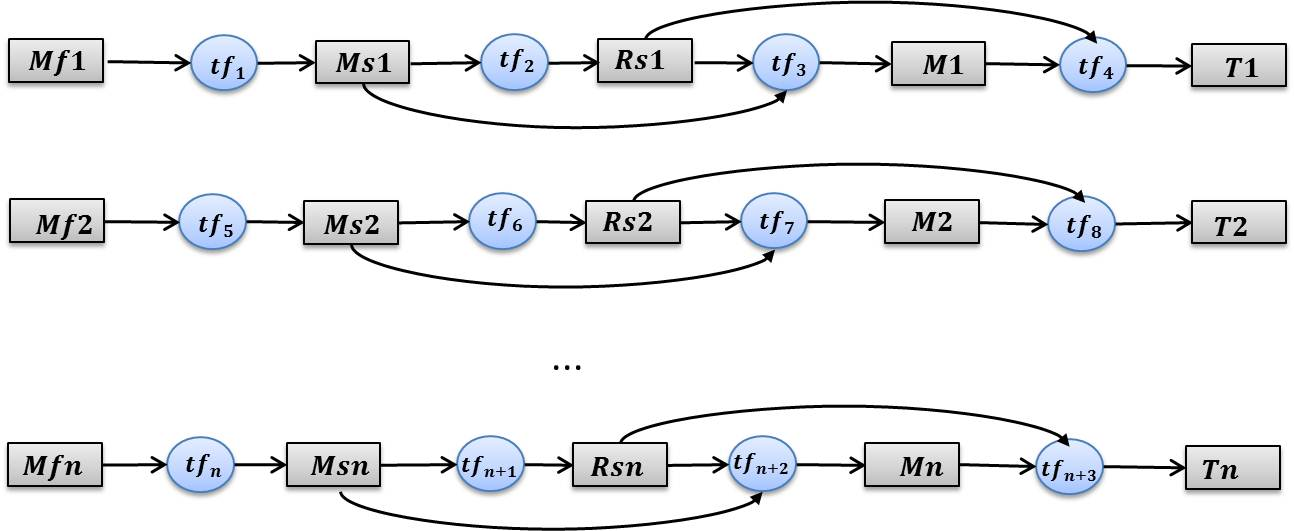
\includegraphics[width=0.8\linewidth]{figure/sciphy.jpg}
\caption{Um grafo representando uma única execução do Sciphy.}
\label{fig:sciphy}
\end{figure}

Como o objetivo é executar uma varredura de parâmetros no Sciphy, cada uma das atividades são executadas com diferentes arquivos de entrada contendo várias sequencias (arquivos multifasta) e, portanto, gerando diferentes tarefas. Cada uma dessas tarefas podem ser executadas em paralelo. Para mais informações sobre o Sciphy, consulte Ocanã \textit{et al.} \cite{ocana2011}.


\subsection{SGWfC SciCumulus}

O SGWfC SciCumulus oferece suporte para dois tipos de paralelismo: varredura de parâmetros \cite{Walker2007}; e paralelismo de dados \cite{Coutinho2010}. O gerenciador atua na distribuição, controle e monitoramento de execuções paralelas de WfCs executados em ambientes de nuvem, e é composto por 4 módulos:

\begin{enumerate}[I]
\item Camada Cliente: Os componentes desse módulo enviam os \textit{workflows} para serem executados na nuvem.
\item Camada de Distribuição: Gera e gerencia  atividades executáveis (tarefas) em uma ou mais MVs instanciadas em um ou mais ambientes de nuvem. 
\item Camada de Execução: É responsável pela execução dos programas invocados pelas atividade do \textit{workflow}, pela geração dos dados e pelo armazenamento dos dados de proveniência.
\item Camada de Dado: Essa camada é base de dados de proveniência, que armazena todos os dados de proveniência consumidos e gerados pela execução paralela do \textit{workflow}. 
\end{enumerate}

O SciCumulus oferece uma infraestrutura computacional mínima para suportar o paralelismo de \textit{workflows} com gerenciamento de dados de proveniência. Para os experimentos apresentados neste trabalho o escalonados do SciCumulus foi modificado. Na versão atual do SciCumulus, o escalonador é baseado em uma abordagem gulosa e dinâmica, chamada  aqui de Greedy-SC \cite{Oliveira2012}. No Greedy-SC sempre que uma máquina fica ociosa o escalonador é chamado para decidir qual será a melhor tarefa a ser executada naquela máquina. Essa é uma abordagem simples que apresenta bons resultados, especialmente quando há variações de performance nas MVs.

% SciCumulus provides the minimal computational infrastructure to support workflow parallelism with provenance management. 
% For the experiments presented in this article the scheduler of SciCumulus had to be modified. In the current and available version of SciCumulus, the scheduler is based on a greedy and dynamic approach. As a VM become idle, it requests a task and then the scheduler decides the best task to be executed in that VM on that specific moment. This is a simple approach and provides good solutions especially when we face performance variations in the VMs, but since it is based on a greedy algorithm, it is not guaranteed that the optimal solution is provided.

Na versão do SciCumulus usada neste experimento, o AEH-ETAA é invocado antes da execução do \textit{workflow}, e são fornecidas as informações das tarefas, dos arquivos e das MVs que formam o \textit{cluster} virtual na nuvem. Todos esses dados são consultados e resgatados dos dados de proveniência \cite{freire2008}. O AEH-ETAA cria então um plano de escalonamento que é retornado para o SciCumulus. O plano de escalonamento é carregado para uma tabela na base de dados, que é consultada pelo escalonar sempre que uma MV fica ociosa. Para mais informações sobre o SciCumulus consulte Oliveira \textit{et al.} \cite{oliveira2010}. 

% In the version of SciCumulus used in this experiment, the HEA-TaSDAP is invoked before each workflow execution. It is provided a list of tasks, the estimated execution time, the number of data files to be produced and consumed and the amount of VMs that are part of the virtual cluster in the cloud. All input data for HEA-TaSDAP is queried and retrieved from the provenance database \cite{freire2008}. HEA-TaSDAP then creates a scheduling plan that is returned to SciCumulus. This scheduled plan is loaded into a database table (since SciCumulus is database-oriented) and this table is queried by the scheduler every time a VM is idle. For more information about SciCumulus, please refer to Oliveira \textit{et al.} \cite{Oliveira2012}. As aforementioned, all scheduling plans provided by HEA-TaSDAP and the executable code will be available on the URL https://bitbucket.org/danielcmo/hea-tasdap. 

\subsection{Configuração do Ambiente}

Os experimentos práticos deste trabalho foram realizados no serviço de nuvem Amazon EC2. O Amazon EC2 é um dos provedores de nuvem comercial mais popular da atualidade, e inúmeras aplicações científicas e comerciais são executadas pelo serviço diariamente. No experimento apresentado neste trabalho foram considerados 2 tipos de MVs oferecidas pelo serviço: m3.small (1 VCpu e 3,75 GB memória RAM) e m3.2xlarge (8 VCpu e 30 GB de memória). As MVs foram definidas conforme as recomendações do GraspCC \cite{Coutinho201551}, uma técnica baseada do GRASP que dimensiona o ambiente de nuvem para WfCs. Segundo o algoritmo de dimensionamento, um ambiente composto por uma m3.small e duas m3.2xlarge seria suficiente para a execução do \textit{workflow} SciPhy.

% For the experiments executed in this article, we have deployed the 2 aforementioned versions of SciCumulus on top of Amazon EC2. Amazon EC2 is the most popular commercial cloud and many scientific and commercial applications are being deployed on it. Amazon EC2 provides several different types of VMs for deployment and use. In the experiments presented in this paper we have considered 2 types of VMs: m3.medium (1 CPU and 3.75 GB RAM) and m3.2xlarge (8 virtual CPU and 30 GB RAM). We have instantiated 1 m3.small and 2 m3.2xlarge following the recommendations of GraspCC \cite{Coutinho201551}, a GRASP-based approach for dimensioning the cloud environment for scientific workflows.


As MVs utilizadas tem como sistema operacional a distribuição Gnu/Linux Cent OS 7 (64 bits), e foram configuradas com os softwares e as bibliotecas necessárias para a execução das aplicações de bioinformática. As máquinas foram instanciadas na região de US East - N. Virginia e  seguem as regras de preço desta localidade. Além disso, as execuções do SciPhy foram realizadas em um único site da Amazon EC2. 

%  Each deployed VM presented in this article is based on the Linux Cent OS 7 (64-bit), and was configured with the necessary software and libraries, and the bioinformatics applications. All VMs were configured to be accessed using SSH. Additionally, these VMs are based on an a AMI image (ami-7e1a1716) that is also stored in the cloud as and SciCumulus creates the virtual cluster to execute the experiment based on this AMI. In terms of software, all VMs, no matter its type, execute the same programs and configurations. All VMs were deployed in the US East - N. Virginia location and follow the pricing rules of that locality. In addition, the executions of SciPhy were performed in a single site of the Amazon EC2 cloud. We did not consider the execution of SciPhy in Multisite clouds neither federated clouds.

\subsection{Configuração do Experimento}

Para executar o SciPhy, foram utilizados como entrada um conjunto de arquivos multifasta contendo sequencias de proteínas extraídas do RefSeq versão 75 - 14 de março, 2016. Esse conjunto de dados é formado por 25 arquivos multifasta de aminoácidos, e cada arquivo é constituído por uma média de 20 sequências. Uma vez baixados, cada arquivo multifasta é armazenado em uma das MVs m3.2xlarge. A fim de gerar arquivos de grande tamanho para o experimento, cada arquivo multifasta teve o seu tamanho artificialmente aumentado. Embora do ponto de vista biológico os resultados produzidos a partir desses arquivos não sejam úteis, pois as sequências foram replicadas inúmeras vezes, a variação no tamanho dos arquivos é fundamental para avaliar a performance dos algoritmos. As seguintes versões dos programas foram utilizadas: MAFFT 6.857, ReadSeq 2.1.22, ModelGenerator 0.85 e RAxML 7.2.8-ALPHA. Para o ModelGenerator, foram considerados os seguintes modelos evolutivos: BLOSUM62, CPREV, HTT, WAG, e RtREV. Cada execução do SciPhy com essa configuração gerou 100 tarefas executáveis e produziu 125 arquivos.


% To execute SciPhy, we have used as input a dataset of multi-fasta files of protein sequences extracted from RefSeq release 75 - March 14, 2016. This dataset is formed by 25 amino acid multi-fasta files and each multi-fasta file is constituted by an average of 20 sequences. Once downloaded, each input multifasta file is stored in one m3.2xlarge VM. In order to generate large data files to the experiment, each multi-fasta file had its size artificially increased. Although this does not produce useful and meaning results from the biological perspective (since the sequences are replicated several times within the same fasta file), it is suitable to evaluate the performance of HEA-TaSDAP. The following program versions were used in the experiments: MAFFT version 6.857 (Multiple Sequence Aligment), ReadSeq 2.1.22 (Sequence Conversion), ModelGenerator version 0.85 (Search for the best evolutionary model) and RAxML-7.2.8-ALPHA (Construction of the phylogenetic tree). For ModelGenerator, we considered the following evolutionary models: BLOSUM62, CPREV, JTT, WAG, and RtREV. Each execution of SciPhy with these configurations generated 100 activity executions and produced 125 data files.

\subsection{Resultados Experimentais do SciPhy}

Nesta subseção são apresentados os tempos de execução do SciPhy utilizando os planos de execução gerados pelos algoritmos Greedy-SC, MinMin, HEFT e AEH-ETAA. Os resultados são apresentados na Figura \ref{fig:boxplot}. Para obter resultados estatísticos significantes, o SciPhy foi executado 5 vezes para cada uma das abordagens. Como apresentado na Figura \ref{fig:boxplot}, o tempo médio de execução do SciPhy foi de $273,1$ minutos para o Greedy-SC, $225,6$ para o MinMin, $214,5$ para o HEFT e $198,2$ minutos para AEH-ETAA. Isso representa aproximadamente $27,4\%$ de melhora quando utilizado AEH-ETAA em comparação com o Greedy-SC, $11,7\%$ em comparação com o MinMin e $8,1\%$ em comparação com o HEFT. Essa diferença é devida a distribuição dos dados feita pelo AEH-ETAA, que alocou os arquivos utilizados por várias tarefas nas MVs com as maiores larguras de banda, diminuindo  assim os tempos de transferências. 

\begin{figure}[H]
\centering
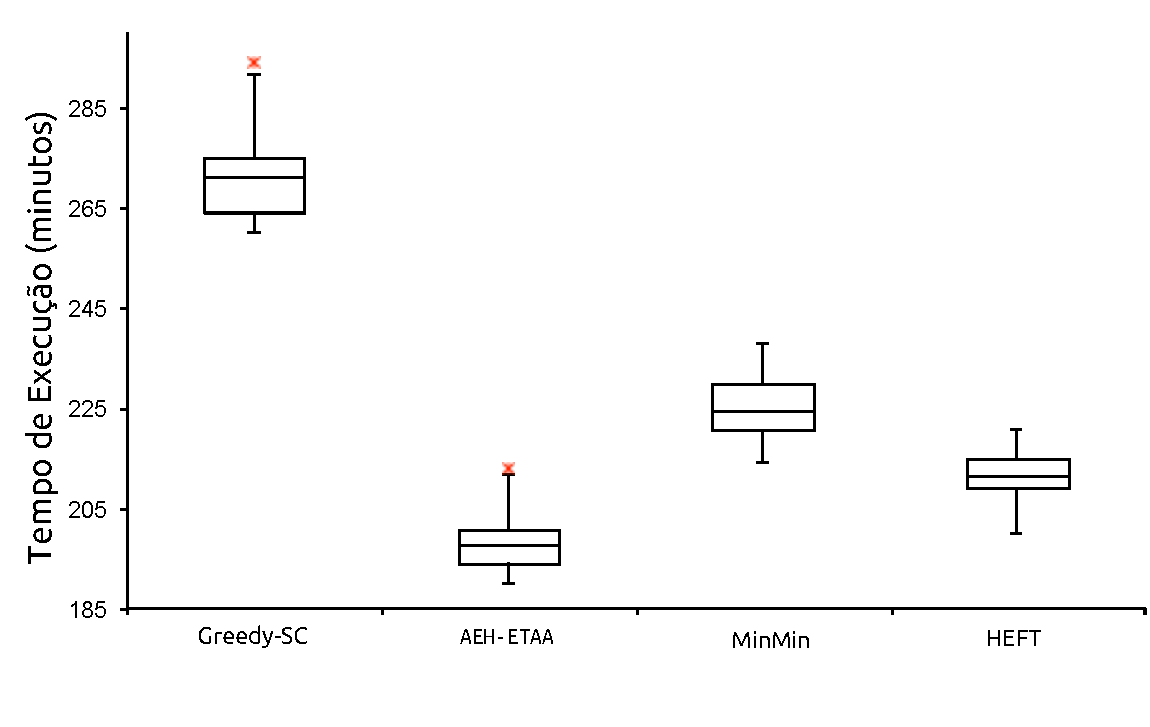
\includegraphics[width=.8\linewidth]{figure/Graphic_FGCS.pdf}
\caption{Diagrama de caixa comparando as execuções do SciPhy utilizando os algoritmos de escalonamento AEH-ETAA, Greedy-SC, HEFT e MinMin.}
\label{fig:boxplot}
\end{figure}



A Tabela \ref{tabelaEstimativa}, apresenta a média dos valores de \textit{makespan} estimados pelos algoritmos estáticos (MinMin, HEFT e AEH-ETAA) em comparação com os valores reais obtidos na execução. Note que os algoritmos estimaram tempos menores em relação aos tempos reais obtidos, representando uma diferença média de mais ou menos $26\%$. Isso ocorre pois tanto os \textit{overheads} oriundos do SciCumulus (como o tempo de consulta à base de dados, por exemplo), quanto as variações de performance das MVs, não são consideradas pelos algoritmos estáticos. Os valores de tempo estimado do algoritmo Greedy-SC não são apresentados, pois como se trata de um algoritmo dinâmico, não há uma estimativa prévia dos tempos de execução do \textit{workflow} escalonado pelo Greedy-SC.
% Todas os valores estatísticos das execuções (mediana, valor minimo, valor máximo, primeiro quartil, terceiro quartil e média) são apresentados na Tabela \ref{resultsciphy}. 


\begin{table}[H]
\small
\begin{center}
\caption{Comparação dos valores estimados e obtidos pelos algoritmos de escalonamento.}
\label{tabelaEstimativa}
\begin{tabular}{|c|c|c|}
\hline
\textbf{Algoritmo} & \textbf{Tempo Estimado} & \textbf{Tempo obtido} \\
\hline
\hline
Greedy-SC   &  \textbf{--} & 273,1\\
MinMin      & 219,31 & 224,6 \\ 
HEFT        & 168,10 & 214,5\\
AEH-ETAA    & 133,36 & 198,2\\
\hline
\end{tabular}
\end{center}
\end{table}	







% This subsection presents the execution time of SciPhy using a greedy scheduling algorithm \cite{Oliveira2012}, MinMin-TSH, HEFT and HEA-TaSDAP scheduling plans in SciCumulus system. The results are presented in Figure \ref{fig:boxplot}. SciPhy was executed 5 times for each approach in order to achieve statistical significance.
% As presented in Figure \ref{fig:boxplot}, the total execution time of SciPhy when using greedy scheduling was of 273.1 minutes in average, was of 224.6 minutes when using MinMin-TSH, was of 214.5 and when using HEA-TaSDAP was of 198.2 minutes in average.
% It represents approximately 27.4\% of improvement when using HEA-TaSDAP in comparison with the greedy algorithm of SciCumulus, 11.7\% of improvement in comparison with MinMin-TSH and 8.1\% of improvement in comparison with HEFT. This difference is due to the data file assignment of HEA-TaSDAP. Most of the bigger data files were placed in VMs with high bandwidth. In case of greedy scheduling and MinMin-TSH, some data files with several GB were placed in VMs with low bandwidth. It is worth mentioning that although HEA-TaSDAP estimated the total execution time in 133.36 minutes, it did not consider variations in the VM performance (which is expected in the cloud environment), the time needed to deploy the VMs in Amazon EC2, to start SciCumulus engine in all VMs involved in the execution and the implicit overhead of querying the database to discover the tasks to execute (~2\% of the total execution time of the workflow).



% In addition, in the execution with the greedy scheduling approach, all data is synchronized for all 3 VMs using Amazon S3, which implies in a certain overhead for every data file produced.
% The overall statistics of the execution (median, min, max, Quartile 1, Quartile 3 and Average) are also presented in Table \ref{resultsciphy}. It is worth noticing that there were no failures neither performance variations in the VMs during the workflow execution. If there were failures or performance variations, the execution using HEA-TaSDAP, HEFT and MinMin-TSH would probably produce worse results since they consider a static set of VMs during the entire execution. Nevertheless, the results are promising and more tests are planned using different workflows such as Montage and Ligo.

% \begin{table}[H]
% \small
% \begin{center}
% \caption{Valores estimados pelos algoritmos de escalonamento}
% \label{resultsciphy}
% \begin{tabular}{|c|c|c|c|c|c|c|}
% \hline
% \textbf{Algoritmo} & \textbf{Média} & \textbf{Mediana} & \textbf{Min} & \textbf{Max} & \textbf{Q1} & \textbf{Q3} \\
% \hline
% \hline
%         Greedy-SC  & 273,1          & 271,0            & 260,3        & 295,9        & 264,1       & 275,2 \\ 
%         AEH-ETAA   & 198,2          & 198,7            & 190,3        & 213,2        & 194,4       & 201,8 \\
%         HEFT       & 214,5          & 211,5            & 198,5        & 221,7        & 209,5       & 215,2 \\
%         MinMin     & 224,6          & 224,6            & 214,2        & 238,0        & 221,9       & 230,6  \\ 
% \hline
% \end{tabular}
% \end{center}
% \end{table}	





% \begin{table}[H]
% \centering
% \caption{Resultados das execuções do SciPhy - Valores em minutos}
% \label{resultsciphy}
% \begin{tabular}{@{}lllllll@{}}
% \hline 
% \toprule
% Approach & Average & Median & Min & Max & Q1 & Q3 \\ \midrule
% \hline 
% Greedy & 273.1 & 271.0 & 260.3 & 295.9 & 264.1 & 275.2 \\ \midrule
% HEA-TaSDAP & 198.2 & 198.7 & 190.3 & 213.2 & 194.4 & 201.8 
% \\ \midrule
% HEFT & 214.5 & 211.5 & 198.5 & 221.7 & 209.5 & 215.2 
% \\ \midrule
% MinMin-TSH & 224.6 & 224.6 & 214.2 & 238.0 & 221.9 & 230.6  \\ \bottomrule
% \end{tabular}
% \end{table}


\chapter{Conclusões e Trabalhos Futuros}\label{chap7}


Experimentos científicos computacionalmente intensivos geralmente produzem um grande volume de dados e apresentam  uma longa duração, na qual várias execuções, utilizando diferentes parâmetros e dados de entrada, são necessárias para obter resultados. Esses experimentos são comumente modelados como \textit{workflows} científicos, que são compostos por uma cadeia de atividades que representam diferentes conjuntos de tarefas. Cada tarefa é associada a uma execução de uma atividade para uma porção especificada dos dados ou para um conjunto de valores de parâmetros. Essas tarefas são executadas em paralelo em ambientes HPC para produzir resultados a um tempo aceitável.

% Data- and compute-intensive scientific experiments usually produce a huge volume of data and present a long duration where several executions, using different parameters and input data, are necessary to draw conclusions. These experiments are commonly modeled as scientific workflows, which are composed by a chain of activities and each activity can be further decomposed in a set of tasks. Each task is associated with the execution of an activity for a specific portion of data or set of parameter values. These tasks have to be executed in parallel in HPC environments to produce results in a feasible time with good performance. 

No entanto, não é trivial gerenciar execuções paralelas de WfCs, particularmente na nuvem. Uma questão importante a ser considerada na execução em ambientes de nuvem é como escalonar as várias tarefas a um conjunto de MVs heterogêneas. O escalonamento de tarefas é um problema NP-Difícil bem conhecido, mesmo na sua forma simples. Além disso, para escalonar as tarefas para MVs várias características devem ser levadas em consideração, tais como a capacidade de processamento, capacidade de armazenamento e o impacto das transferências de dados no tempo total de execução. Este trabalho parte da ideia de que o problema de escalonamento de tarefas e o problema de alocação de dados não são independentes e, portanto, devem ser analisados de forma conjunta pela abordagem de escalonamento. 

% However, it is far from trivial to manage the parallel executions of data- and compute-intensive scientific workflows, particularly in clouds. One important issue to consider when executing workflows in parallel in clouds is how to schedule the multiple tasks to a set of heterogeneous VMs. Task scheduling is a well-known NP-complete problem even in its simplest form. But to schedule the tasks to VMs we have to consider several requirements such as the processing capacity of the VM, its storage capacity and the impact of data transfer. In this article we claim that data distribution and task distribution are not independent problems and have to be analyzed together by the scheduling approach. In previous work \cite{Oliveira2012} we have addressed workflow execution in clouds using a greedy scheduling algorithm but it does not consider data placement in the scheduling algorithm, which may imply in severe overheads. Thus, to increase the uptake of the cloud paradigm for executing scientific workflows that demand HPC capabilities, new scheduling solutions have to be developed.  

Neste trabalho, um novo modelo de representação de \textit{workflow} foi proposto, junto a uma formulação matemática do problema de escalonamento de dados e distribuição de tarefas e um algoritmo de escalonamento evolutivo hibrido chamado AEH-ETAA que considera a heterogeneidade das MVs no ambiente de nuvem (diferentes larguras de banda, capacidade de processamento e armazenamento), a distribuição dos dados e as restrições, todos juntos na mesma solução, ou seja, as tarefas e os arquivos são escalonados juntos pelo SGWfC.

% In this article,  we propose a new  model  for representing workflows, a mathematical formulation of The Task Scheduling and Data Assignment Problem and a scheduling algorithm based on Hybrid Evolutionary Algorithm (HEA) named HEA-TaSDAP that takes into account the variety and heterogeneity of VMs in cloud virtual cluster (\textit{e.g.} different bandwidths, transfer rates, and processing capacities), the data distribution and data constraints all together within the same solution, \textit{i.e.} tasks and data files are scheduled together by the SWfMS.

O AEH-ETAA foi avaliado utilizando \textit{workflows} sintéticos e reais utilizando o SGWfCs SciCumulus. A avaliação de performance do AEH-ETAA em comparação com a solução exata, mostrou que, para todas as instâncias, o AEH-ETAA obtém boas soluções com pequenas diferenças percentuais, na média $2,6\%$. Além disso, o algoritmo  leva um tempo significativamente menor quando comparado à formulação matemática solucionada com o CPLEX, em média $1,5$s contra $1942,7$s, respectivamente. Na execução real, foi utilizado o SciPhy como estudo de caso para a comparação do AEH-ETAA com o algoritmo guloso do SciCumulus Greedy-SC, MinMin e HEFT. O tempo de execução do SciPhy quando executado com o plano de escalonamento dado pelo AEH-ETAA foi em torno de $27,4\%$ menor que o dado pelo algoritmo guloso, $11,7\%$ menor que o MinMin e $8,1\%$ menor que o HEFT. 

Como trabalhos futuros, a abordagem proposta será incrementado com técnicas de tolerância a falhas que  realizarão \textit{backups} das tarefas, e possibilitarão a recuperação parcial, ou total, dos processos caso haja interrupções devido a ocorrência de falhas no ambiente. Além disso, também serão adotadas técnicas de redimensionamento do ambiente que serão capazes de alocar e desalocar as MVs durante a execução do \textit{workflow}. As técnicas de redimensionamento são importantes nos ambientes de nuvens, pois possibilitam diminuir o custo financeiro associado ao ambiente. Outro trabalho interessante é a inclusão de outros objetivos (abordagem multiobjetivo) no modelo proposto, como minimizar os custos financeiros e o \textit{makespan}, respeitando o tempo limite de execução definido pelo usuário e um valor máximo de orçamento. 

% We have evaluated HEA-TaSDAP using synthetic and real workflows in the cloud using SciCumulus. The performance evaluation of the HEA-TasDAP using synthetic workflows in comparison with the exact solution showed that for all instances HEA-TaSDAP obtains good solutions with small gaps, in average $2.6\%$. Moreover, it takes significantly less time when compared with the mathematical formulation when solved with the CPLEX, in average $1.5$s against $1942.7$s, respectively. In the real execution, we used SciPhy as a case study and compared HEA-TaDASP with the greedy scheduling of SciCumulus, MinMin-TSH and HEFT. The execution time of SciPhy when using the scheduling plan provided by HEA-TaSDAP was about 27.4\% smaller than the one using the greedy algorithm, 11.7\% smaller than MinMin-TSH and 8.1\% smaller than using HEFT. As future work, we plan to use the proposed approach in conjunction with a fault-tolerance and a dimensioning mechanism within the scheduler to distribute backups of tasks and then execute the workflow with more reliability. Another interesting work could involve considering  other objectives in our model like  minimization of  financial costs and power consumption, respecting tasks deadlines. Finally, we also intend to tackle the data replication problem in our models, as previous commented in Section \ref{sec:problemDef}.





% --- -----------------------------------------------------------------
% --- Referencias Bibliograficas. (Obrigatorio)
% --- -----------------------------------------------------------------
\cleardoublepage
\bibliographystyle{acm-2} % abbrv - abnt-num
%\bibliographystyle{uff-ic}
\bibliography{bibliografia} % arquivo fonte com a bibilografia

% --- -----------------------------------------------------------------
% --- Apendice.(Opcional)
% --- -----------------------------------------------------------------
% \cleardoublepage
% \appendix
% \chapter{<T\'ITULO DO AP\^ENDICE>}
\label{apend}

% Este ap�ndice apresenta informa��es complementares.

Elemento opcional. O(s) ap�ndice(s) s�o identificados por letras mai�sculas consecutivas, travess�o e pelos respectivos t�tulos. Excepcionalmente utilizam-se letras mai�sculas dobradas, na identifica��o, quando esgotadas as 23 letras do alfabeto (ABNT, 2005).


\end{document}

